\documentclass[12pt, a4paper, oneside]{book}

% === PACKAGES ===
\usepackage[hidelinks, breaklinks=true]{hyperref} % Load hyperref once, early

\usepackage{setspace}
\usepackage{graphicx} % needed for images
\usepackage[utf8]{inputenc} % Input encoding
\usepackage[english]{babel} % For English thesis

% Fix for "\iint already defined" error before loading amsmath
\let\iint\relax
\let\iiint\relax
\let\iiiint\relax
\let\idotsint\relax 
% The lines above undefine these specific commands if they were previously defined by another package,
% allowing amsmath to define them without conflict.

\usepackage{amsmath} % For math symbols
\usepackage{amsfonts} % For other math fonts/symbols
\usepackage{amssymb} % For more math symbols
\usepackage{geometry} % For adjusting margins
\usepackage{appendix} % For better appendix handling with hyperref
\usepackage{subcaption} % For subfigure environment
\geometry{a4paper, margin=1.2in}
\usepackage{longtable} % For the large component table
\usepackage{tabularx} % For other tables
\usepackage{times} % Font often used in theses
\usepackage{float} % To control figure/table placement better e.g. [H]
\usepackage{caption} % For better control over captions
\usepackage{booktabs} % For nicer table lines
\usepackage{xcolor} % Needed for color names
\usepackage{listings} % Added for improved code listings
\usepackage{rotating} % Added for landscape figures
\usepackage{tikz} % Added for native flowcharts and diagrams
\usetikzlibrary{shapes.geometric, arrows.meta, positioning}

% Added packages for the component table
\usepackage{array} % For \newcolumntype and better column control
\usepackage{makecell} % For \makecell and \newline in cells
\usepackage{colortbl} % For \cellcolor

% Define raggedright paragraph column type to avoid underfull hbox warnings
\newcolumntype{L}[1]{>{\raggedright\arraybackslash}p{#1}}

% === LISTINGS PACKAGE SETUP ===
\definecolor{codegreen}{rgb}{0,0.6,0}
\definecolor{codegray}{rgb}{0.5,0.5,0.5}
\definecolor{codepurple}{rgb}{0.58,0,0.82}
\definecolor{backcolour}{rgb}{0.98,0.98,0.98} % Light gray background for code

\lstdefinestyle{mystyle}{
    backgroundcolor=\color{backcolour},
    commentstyle=\color{codegreen},
    keywordstyle=\color{magenta},
    numberstyle=\tiny\color{codegray},
    stringstyle=\color{codepurple},
    basicstyle=\footnotesize\ttfamily,
    breakatwhitespace=false,
    breaklines=true,
    captionpos=b,
    keepspaces=true,
    numbers=left,
    numbersep=5pt,
    showspaces=false,
    showstringspaces=false,
    showtabs=false,
    tabsize=2,
    language=Python,
    morekeywords={const, unique_id, ubinascii}, % Add MicroPython specific keywords
    emph={BLEUART, PWM, Pin}, emphstyle=\color{blue}\bfseries, % Emphasize custom classes/key objects
    postbreak=\mbox{\textcolor{red}{$\hookrightarrow$}\space}, % Symbol for continued lines
    frame=tb, % Adds a top and bottom frame
    framesep=3pt,
    framerule=0.5pt,
}
\lstset{style=mystyle}


% === PATHS ===
% Define paths to avoid long file paths in includegraphics
\newcommand{\litreviewpath}{images/literature/}
\newcommand{\taskthreepath}{images/}


% === GUC TEMPLATE DEFINITIONS ===
\newcommand{\submissionDay}{22}
\newcommand{\submissionMonth}{June}
\newcommand{\submissionYear}{2025}
\newcommand{\submissionDate}{\submissionDay~\submissionMonth,~\submissionYear}
\newcommand{\typeOfThesis}{Bachelor Thesis}

\newcommand{\titleOfThesisOne}{Design and Implementation of a Smart Cleaning Robot} % Title
\newcommand{\authorOfThesis}{Andrew Khalil Samuel Abdelmalak} % My Name
\newcommand{\supervisorOne}{Prof. Dr. Walid Atef Hafez Omran} % Supervisor
\newcommand{\cosupervisor}{Dr. Hisham Mostafa El Sherif} % Co-Supervisor
\newcommand{\reviewer}{Dr. M. A. Moustafa Hassan} % Reviewer

% === Table specific settings and new commands from component list ===
\setlength{\LTleft}{0pt plus 1fil}
\setlength{\LTright}{0pt plus 1fil}
\setlength{\tabcolsep}{5pt} % Column separation for longtable

\definecolor{darkblue}{RGB}{0,0,128}
\definecolor{lightgray}{RGB}{240,240,240}

% ==== Electrical Totals ====
\newcommand{\totalVoltage}{12V}      % Battery voltage
\newcommand{\totalCurrent}{~2.2A}      % Recalculated total current @12V
\newcommand{\totalPower}{~26W}       % Recalculated total power consumption

% A little extra stretch to prevent warnings globally
\setlength{\emergencystretch}{1em}


% === DOCUMENT START ===
\begin{document}

% Front matter (title page, abstract, TOC, lists)
\frontmatter % Use for roman page numbering, ToC, lists, etc.
\pagestyle{plain}

% --- Title Page Definition ---
\newcommand{\titlePage}{
  \thispagestyle{empty}
  \begin{center}
    \textbf{Faculty of Engineering and Materials Sciences}\\[1mm]
    \textbf{German University in Cairo}\\[1mm]
    
\includegraphics[width=0.1\textwidth, keepaspectratio]{images/misc/guc_logo.png}

    \vspace{2cm}
    \doublespacing
    {\Huge \textbf{\titleOfThesisOne}}\\
    \singlespacing
    \vspace{2cm}
    {\large \textbf{\typeOfThesis}}\\

    \vfill
    \parbox{10cm}{ % Adjusted width slightly for potentially longer names
      \begin{large}
        \begin{tabbing} % Used tabbing for alignment
          Author: \hspace{2.5cm} \=\authorOfThesis\\[2mm] % Adjusted spacing
          Supervisors: \> \supervisorOne\\[2mm]
          Co-Supervisor: \> \cosupervisor\\[2mm]
          Reviewer: \> \reviewer\\[2mm]
          Submission Date: \> \submissionDate\\
        \end{tabbing}
      \end{large}
    }
  \end{center}
  \clearpage
}
% Call the title page command
\titlePage

% --- Certification Page Inclusion ---
\thispagestyle{empty}
This is to certify that:
\begin{itemize}
\item[(i)] the thesis comprises only my original work toward the Bachelor Degree
\item[(ii)] due acknowledgement has been made in the text to all other material used
\end{itemize}

\vspace{3cm} % Increased spacing
\begin{flushright}
\rule[0mm]{6cm}{0.2mm}\\ % Signature line
\vspace{5mm} % Space before name
\authorOfThesis\\
\submissionDay~\submissionMonth,~\submissionYear\\
\end{flushright}
\clearpage

% --- Acknowledgements Inclusion ---
\chapter*{Acknowledgements}
\addcontentsline{toc}{chapter}{Acknowledgements} % Adds this page to the Table of Contents

I would first like to thank God for granting me the strength, focus, and perseverance to complete this work.

\vspace{1em}

I am deeply grateful to my supervisor, \supervisorOne, whose expertise in electrical engineering, patient guidance, and enthusiastic encouragement were invaluable throughout every stage of this thesis.

\vspace{1em}

I would also like to express my sincere appreciation to my co-supervisor, \cosupervisor, whose mechanical-engineering perspective and constructive feedback greatly enriched both the research and the writing of this work.

\vspace{1em}

Finally, I wish to thank my parents and family for their unwavering support, patience, and constant encouragement.

\vspace{2cm}
\begin{flushright}
\authorOfThesis\\
\submissionDate\\
\end{flushright}
\clearpage

% --- Dedication ---
\chapter*{Dedication}
\thispagestyle{empty}
\vspace*{3cm}
\begin{center}
\textit{To my parents,\\[0.5em]
for their endless support, patience,\\[0.5em]
and unwavering belief in me.}
\end{center}
\clearpage

% --- Abstract Inclusion ---
\chapter*{Abstract}
\addcontentsline{toc}{chapter}{Abstract} % This link for Abstract is usually fine
Household cleaning is a repetitive and time-consuming task, often detracting from other valuable activities in increasingly busy modern lifestyles. This project addresses the persistent need for automation in domestic environments by focusing on the critical area of floor cleaning, aiming to alleviate this burden. The primary objective is the comprehensive design, development, and implementation of a ``Smart Cleaning Robot'' prototype, conceived to simplify cleaning routines and significantly reduce direct human effort and interaction. This thesis meticulously details the iterative development journey of this prototype, from conceptualization through multiple design refinements to final assembly.

The robot's navigation has been engineered into a hybrid feed-forward and feedback control system, utilizing a predictive model to proactively manage motor commands while using a Proportional-Integral-Derivative architecture to correct for real-world deviations. This enables the robot to navigate more methodically using a coverage pattern of moving forward until an obstacle is detected and then executing a wide, corrective turn. This system allows it to manage its movements with greater precision and perform autonomous recovery maneuvers. The robot's core functionality relies on an integrated vacuum system, powered by a PS3 Slim fan. Central control is managed by a Raspberry Pi Pico W microcontroller, which processes data from an ultrasonic distance sensor for real-time obstacle detection and from the encoders for motion control. Mobility is achieved through two independently controlled Direct Current motors, and the entire system is powered by a rechargeable Lithium-ion battery pack.

The project's methodology encompassed a structured, iterative design process that included detailed mechanical modeling using SolidWorks software, the fabrication of a custom 3D-printed chassis, and the design and implementation of a dedicated Printed Circuit Board. The prototype achieves its core functionality at approximately 60--90\% lower cost than entry-level commercial robots, with a total component cost of approximately \$80 USD. Testing demonstrated stable BLE remote control, improved navigation precision through PID control, and an operational battery runtime exceeding 60 minutes. While the prototype successfully demonstrates effective vacuuming and responsive remote control, the core of the work lies in the implementation and analysis of the advanced control system. This thesis candidly highlights the successes in implementing this system, the remaining precision challenges inherent to the chosen hardware, and the key recommendation of exploring stepper motors for future work, thereby contributing to the accessibility of domestic robotic assistance.
\clearpage % Ends the Abstract page. ToC will start on a new page.

% --- Table of Contents ---
\phantomsection % Add an anchor for hyperref at the top of the new page
\addcontentsline{toc}{chapter}{Table of Contents} % Link the ToC entry to the anchor above
\renewcommand{\contentsname}{Table of Contents} % Define the title string for \tableofcontents
\tableofcontents % This prints the actual Table of Contents
\clearpage

% --- List of Figures ---
\phantomsection % Add an anchor for hyperref at the top of the new page
\addcontentsline{toc}{chapter}{List of Figures} % Link the LoF entry to this anchor
\listoffigures % This prints the actual List of Figures
\clearpage

% --- List of Tables ---
\phantomsection % Add an anchor for hyperref at the top of the new page
\addcontentsline{toc}{chapter}{List of Tables} % Link the LoT entry to this anchor
\listoftables % This prints the actual List of Tables
\clearpage

% --- List of Abbreviations ---
\chapter*{List of Abbreviations}
\addcontentsline{toc}{chapter}{List of Abbreviations}
\begin{description}
    \item[\textbf{ADC}:] Analog-to-Digital Converter. \label{term:adc}
    \item[\textbf{BLE}:] Bluetooth Low Energy. \label{term:ble}
    \item[\textbf{CAD}:] Computer-Aided Design. \label{term:cad}
    \item[\textbf{DC}:] Direct Current. \label{term:dc}
    \item[\textbf{FDM}:] Fused Deposition Modeling. \label{term:fdm}
    \item[\textbf{FF}:] Feed-Forward. \label{term:ff}
    \item[\textbf{GPIO}:] General Purpose Input/Output. \label{term:gpio}
    \item[\textbf{HC-SR04}:] Ultrasonic Sensor Model. \label{term:hcsr04}
    \item[\textbf{IDE}:] Integrated Development Environment. \label{term:ide}
    \item[\textbf{IMU}:] Inertial Measurement Unit. \label{term:imu}
    \item[\textbf{IR}:] Infrared. \label{term:ir}
    \item[\textbf{L298N}:] H-Bridge Motor Driver Model. \label{term:l298n}
    \item[\textbf{LDS}:] Laser Direct Structure. \label{term:lds}
    \item[\textbf{LED}:] Light Emitting Diode. \label{term:led}
    \item[\textbf{LiDAR}:] Light Detection and Ranging. \label{term:lidar}
    \item[\textbf{Li-ion}:] Lithium-ion. \label{term:liion}
    \item[\textbf{PCB}:] Printed Circuit Board. \label{term:pcb}
    \item[\textbf{PID}:] Proportional-Integral-Derivative. \label{term:pid}
    \item[\textbf{PLA}:] Polylactic Acid. \label{term:pla}
    \item[\textbf{PWM}:] Pulse Width Modulation. \label{term:pwm}
    \item[\textbf{ROS}:] Robot Operating System. \label{term:ros}
    \item[\textbf{RPLidar}:] Rotating Light Detection and Ranging sensor model. \label{term:rplidar}
    \item[\textbf{RPM}:] Revolutions Per Minute. \label{term:rpm}
    \item[\textbf{SBC}:] Single-Board Computer. \label{term:sbc}
    \item[\textbf{SLAM}:] Simultaneous Localization and Mapping. \label{term:slam}
    \item[\textbf{UART}:] Universal Asynchronous Receiver-Transmitter. \label{term:uart}
    \item[\textbf{VBUS}:] USB Voltage Bus. \label{term:vbus}
    \item[\textbf{vSLAM}:] Visual Simultaneous Localization and Mapping. \label{term:vslam}
\end{description}
\clearpage


% --- List of Symbols ---
\chapter*{List of Symbols}
\addcontentsline{toc}{chapter}{List of Symbols}
\begin{description}
    \item[\textbf{V}:] Voltage (\textit{Volts})
    \item[\textbf{I}:] Current (\textit{Amperes})
    \item[\textbf{P}:] Power (\textit{Watts})
    \item[\textbf{R}:] Resistance (\textit{Ohms})
    \item[\textbf{f}:] Frequency (\textit{Hertz})
    \item[\textbf{T}:] Time Period (\textit{Seconds})
    \item[\textbf{D}:] Duty Cycle
    \item[\textbf{$\theta$}:] Angle (\textit{Degrees})
    \item[\textbf{L}:] Length (\textit{cm/m})
    \item[\textbf{W}:] Width (\textit{cm/m})
    \item[\textbf{H}:] Height (\textit{cm/m})
    \item[\textbf{m}:] Mass (\textit{kg/g})
    \item[\textbf{gf.cm}:] Gram-force centimeter (\textit{Torque unit})
\end{description}
\clearpage

% Main content chapters
\mainmatter % Switch to Arabic page numbering and reset chapter count for main body
% --- Chapter 1: Introduction ---
\chapter{Introduction}
\label{chap:intro}

\section{Motivation}
\label{sec:motivation_intro}
Keeping our homes and workplaces clean is important for a healthy and pleasant life. But cleaning floors by hand often takes a lot of time, is boring, and can be hard physical work. In today's busy world, people have many things to do. Finding enough time and energy for regular cleaning can be tough, especially in big homes or busy business places. New technologies, especially in robotics, offer a good solution. Cleaning robots, which were once just an idea, are now helpful tools. They make cleaning easier, do a consistent job, and most importantly, save people's time. This saved time can be used for other important tasks, learning new things, or relaxing. The development of this technology has not only changed how we do chores but has also created new business opportunities and markets. For example, companies like iRobot, with its famous Roomba, were pioneers. They showed that many people wanted these new cleaning robots. After that, big home appliance companies like Samsung, LG, Dyson, and SharkNinja, and robot companies like Ecovacs and Roborock, also started making their own cleaning robots. They saw it as an important and growing part of the smart home market. This shows how automated cleaning has made a big impact, turning a new idea into a large global business.
This project looks at cleaning in Egyptian homes. In Egypt, many floors are made of tile or marble. Also, some areas can have a lot of dust. These conditions make automated cleaning robots very useful. Many advanced cleaning robots are sold worldwide, but they can be very expensive for some people. Because of this, and because people might want robots that fit their specific needs, there's a chance to create simpler, effective robots that can be made or put together locally. So, the main reason for this bachelor thesis is to design and build a smart cleaning robot that works well, is practical, and doesn't cost too much. The goal is to make a robot that greatly cuts down on the handwork needed for common floor cleaning, making homes more efficient and life easier. This project tries to find a good balance between useful features and cost, offering a helpful step in home robotics.

\section{Aim of the project}
\label{sec:aim_intro}
The primary technical aim of this work is to design and implement a functional prototype of a smart cleaning robot. This robot is intended to automate common floor cleaning tasks, thereby reducing manual effort and enhancing convenience within a typical household environment. The project focuses on delivering a practical and cost-effective solution that balances essential functionalities with simplicity of operation. The specific tasks to achieve this aim involve the implementation of the following core robot functions:
\begin{itemize}
    \item \textbf{Automated Vacuum Cleaning:} The robot will be equipped with a vacuuming system capable of collecting common household dust and light debris from floor surfaces. This function is central to its cleaning purpose.
    \item \textbf{Enhanced Autonomous Navigation:} The robot will implement a hybrid feed-forward and \hyperref[term:pid]{PID} control system using wheel encoders. The aim is to significantly improve movement precision, enabling the robot to more reliably execute a systematic room coverage pattern based on its sensor feedback. The system will also include autonomous stall detection and a recovery sequence.
    \item \textbf{Remote Control Operation:} The robot will feature a \hyperref[term:ble]{BLE} remote-control interface, enabling users to manually guide its movements. This is enhanced by \hyperref[term:pid]{PID} control to maintain a straight path during forward motion and an automatic obstacle-stop safety feature.
    \item \textbf{User Feedback System:} The robot will incorporate basic visual indicators (e.g., an \hyperref[term:led]{LED}) to provide feedback to the user about its current operational status.
\end{itemize}
The successful implementation and qualitative verification of these functions will demonstrate the achievement of the project's technical aim. This project aims to deliver a foundational smart cleaning robot prototype, with the understanding that highly advanced features like sophisticated mapping (\hyperref[term:slam]{SLAM}) are outside the current scope.

\section{Thesis Structure}
\label{sec:structure_intro_section}
This thesis is organized into five chapters. Each chapter discusses a different part of the project, providing a clear and logical progression from initial concepts to final outcomes and future possibilities: % Updated chapter count

\begin{itemize}
    \item \textbf{\hyperref[chap:intro]{Chapter 1: Introduction (This Chapter)}} This chapter provides the background for the project. It explains the motivation for developing a smart cleaning robot, outlines the project's objectives, and details the organization of this document.
    \item \textbf{\hyperref[chap:background]{Chapter 2: Theoretical Background and Literature Review}} This chapter delves into the technologies, design principles, and prior research relevant to autonomous and semi-autonomous cleaning robots. It examines various non-commercial and commercial robot designs, focusing on their navigation strategies, sensing capabilities, cleaning mechanisms, and control systems. It also reviews specific path planning techniques like the boustrophedon pattern.
    \item \textbf{\hyperref[chap:mechanical_design_assembly]{Chapter 3: Mechanical Design and Assembly}} This chapter focuses on the physical construction of the robot. It details the selection of mechanical components, the SolidWorks-based design of the chassis and custom parts, the selection of materials, the mechanical assembly process, and the specifics of the vacuum system's mechanical integration.
    \item \textbf{\hyperref[chap:electrical_control_performance]{Chapter 4: Electrical and Control System Design and Testing}} This chapter describes the electronic ``brains and nerves'' of the robot. It covers the selection of electrical components, the overall system architecture centered on the Raspberry Pi Pico W, the detailed electrical design and integration including the custom \hyperref[term:pcb]{PCB}, and the embedded software development for control. Finally, it presents a qualitative performance evaluation of the assembled prototype.
    \item \textbf{\hyperref[chap:conclusion_future_work_new]{Chapter 5: Conclusion and Recommendations for Future Work}} This chapter summarizes the project's main achievements and findings. It reflects on the extent to which the initial goals were met, discusses the identified limitations, and proposes recommendations for future research and potential improvements to enhance the robot's functionality and performance.
\end{itemize}

This structured approach aims to provide a comprehensive account of this project from its inception to its current state.
% --- Chapter 2: Theoretical Background and Literature Review ---
\chapter{Theoretical Background and Literature Review}
\label{chap:background}

This chapter gives a broad look at the main technologies, common design methods, and important past work related to cleaning robots that work by themselves or with some human help. By looking at existing research, non-commercial projects, and store-bought robots, this review will help create a strong base of knowledge for the design choices made in this thesis. The chapter will explore key areas like how robots move around, how they detect and avoid objects, different ways they clean, how their control systems work, and how they manage power. It will also touch upon specific coverage patterns relevant to systematic cleaning.

\section{Overview of Cleaning Robot Technologies}
\label{sec:overview_tech_lit}
Automated cleaning robots have changed a lot over the years. They started as simple machines and have become much smarter. This happened because of better sensors, more powerful computer chips, and improved software that help them work more independently and effectively.

\subsection*{Robotic Navigation and Environmental Mapping Strategies}
A robot's ability to navigate its environment effectively is fundamental. Various techniques exist, ranging in complexity and the level of autonomy they provide:
\begin{itemize}
    \item \textbf{Basic Reactive Strategies:} These are the simplest forms of navigation.
        \begin{itemize}
            \item \textit{Random Walk:} The robot moves until an obstacle is detected (e.g., by a bump sensor), then changes direction, often randomly. This is low-cost but inefficient for coverage.
            \item \textit{Predefined Path Following and Algorithmic Patterns:} Robots may follow a set path or execute geometric patterns (spirals, wall-following). These offer more structure than random walks and can use simple sensors like line-followers or odometry (wheel tracking) with basic proximity sensors for obstacle avoidance. They are best for known, uncluttered spaces. A fundamental component for odometry is the wheel encoder, a sensor that measures the rotation of the wheels. By counting the rotational ``pulses,'' the robot can calculate the distance it has traveled with high precision, enabling more reliable execution of systematic coverage patterns.
        \end{itemize}
    \item \textbf{Systematic Coverage Path Planning:} For more thorough cleaning, robots aim to cover an entire accessible area without unnecessary repetition. A common approach for this is the boustrophedon pattern (also known as an ox-plowing or lawnmower pattern)~\cite{Choset2001Coverage}. This involves moving back and forth in parallel lines, much like mowing a lawn, to ensure complete coverage of a rectangular area. Figure~\ref{fig:boustrophedon_pattern_placeholder} illustrates this pattern. Achieving this reliably requires accurate localization and control, often using wheel encoders or more advanced sensing. While this systematic pattern represents a common and efficient goal in robotics, the prototype developed in this thesis implements a simpler coverage strategy based on direct sensor feedback as a practical step toward this ideal, working within the precision limits of the available hardware.
        \begin{figure}[htbp]
            \centering
            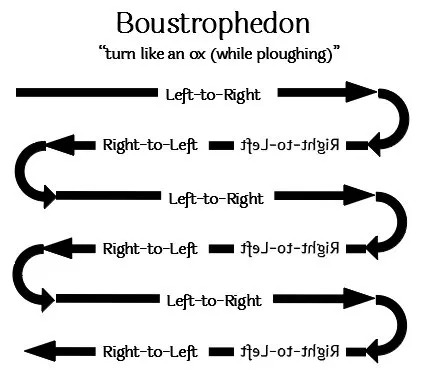
\includegraphics[width=0.75\textwidth, keepaspectratio]{images/literature/boustrophedon_pattern.jpg}
            \caption{Illustration of the Boustrophedon coverage path pattern.}
            \label{fig:boustrophedon_pattern_placeholder}
        \end{figure}
    \item \textbf{Advanced Mapping and Localization:} \hyperref[term:slam]{SLAM} represents a major step in autonomy~\cite{Cadena2016PastPresentFutureSLAM}, allowing a robot to build a map of an unknown area while simultaneously tracking its position. This results in a much more efficient and systematic cleaning path compared to random navigation (Figure~\ref{fig:slam_comparison}).\\
        \begin{figure}[htbp]
            \centering
            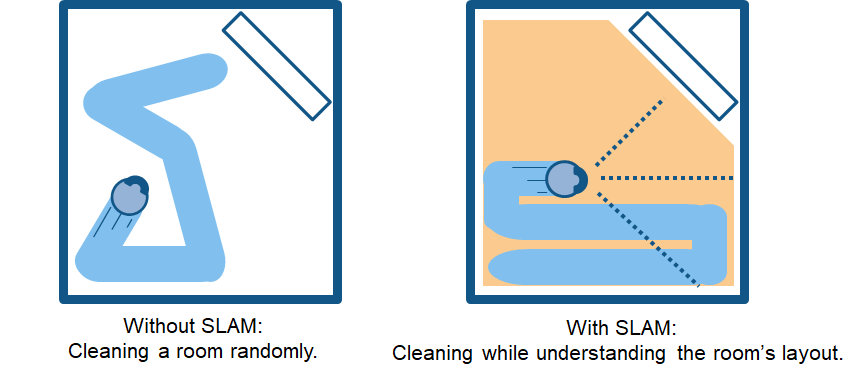
\includegraphics[width=1\textwidth]{images/literature/slam_comparison.png}
            \caption{A comparison of a random navigation path versus a systematic path enabled by \hyperref[term:slam]{SLAM} (Concept from~\cite{mathworks_slam}).}
            \label{fig:slam_comparison}
        \end{figure}
    This is computationally intensive and relies on rich sensor data (like from \hyperref[term:lidar]{LiDAR} or cameras) to create a spatial awareness map, which can be a 2D grid or a more complex 3D point cloud, as shown in Figure~\ref{fig:slam_3d_map}.
        \begin{figure}[htbp]
            \centering
            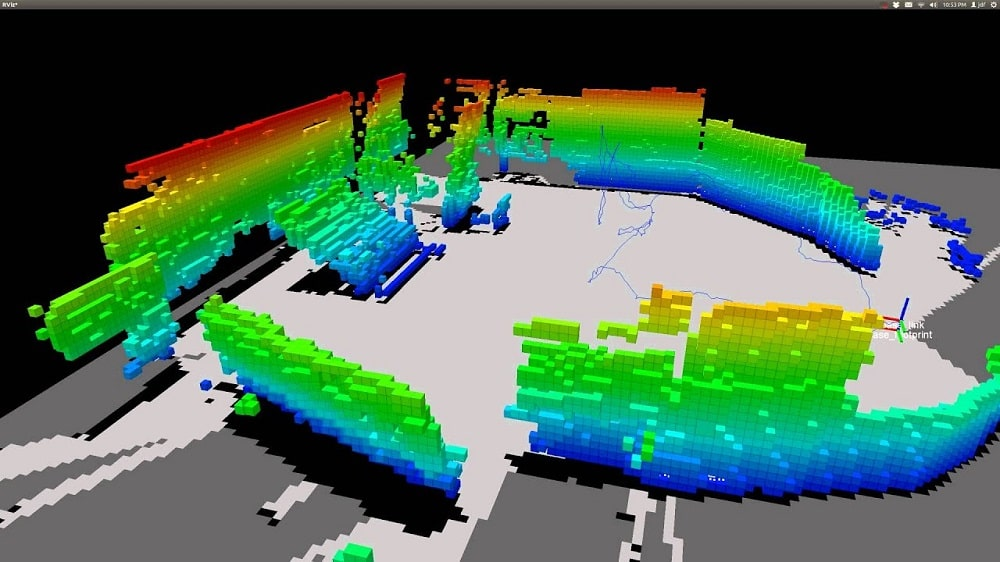
\includegraphics[width=0.97\textwidth]{images/literature/slam_3d_map.jpg}
            \caption{An example of a 3D point-cloud map of an environment generated using \hyperref[term:slam]{SLAM} (Concept from~\cite{geospatialnext_slam}).}
            \label{fig:slam_3d_map}
        \end{figure}
    \item \textbf{\hyperref[term:pid]{PID} Feedback Control:} To achieve the precision needed for systematic patterns, a feedback control loop is essential. The Proportional-Integral-Derivative (\hyperref[term:pid]{PID}) controller is a ubiquitous and robust method used for this purpose. It continuously calculates an error value between a desired setpoint and a measured process variable and applies a correction based on proportional, integral, and derivative terms. A detailed explanation of this control method, as it applies to this project, is provided in the following section.
\end{itemize}

\subsubsection{Principles of \texorpdfstring{\hyperref[term:pid]{PID}}{PID} Feedback Control}
\label{subsubsec:pid_principles}
To move beyond simple reactive strategies, a feedback control system is necessary to allow the robot to correct its own errors in real-time. The most common and robust method for this is the \textbf{Proportional-Integral-Derivative (\hyperref[term:pid]{PID})} controller~\cite{AerospaceControlsLab2016PID}. A \hyperref[term:pid]{PID} controller works by calculating an ``error'' value---the difference between a desired setpoint (e.g., a target wheel speed) and the current measured value---and then calculating a corrective action to apply to the system (e.g., motor power). The power of the \hyperref[term:pid]{PID} controller comes from its three distinct terms, each addressing a different aspect of the error.
\begin{itemize}
    \item \textbf{The Proportional (P) Term: Reacting to the Present}\\
    The Proportional term provides a response that is directly proportional to the current error. If the error is large, the corrective action is large; if the error is small, the correction is small. For our robot driving straight, the error could be the difference in speed between the two wheels. The P-term works to make this error zero. However, relying on the P-term alone can lead to instability. A high proportional gain (the scaling factor, $K_p$) can cause the system to \textbf{overshoot} the target, oscillating back and forth around the setpoint.
    \item \textbf{The Derivative (D) Term: Predicting the Future}\\
    The Derivative term works to counteract this overshoot. It looks at the \textbf{rate of change} of the error. If the error is decreasing rapidly (meaning the robot is quickly approaching its target), the D-term will apply a damping force to slow the correction down, preventing overshoot. It essentially acts as a brake, adding resistance against rapid changes and making the system's response smoother. Properly tuning the derivative gain ($K_d$) leads to a ``\textbf{critically damped}'' system that approaches the target quickly but without oscillation.
    \item \textbf{The Integral (I) Term: Correcting for the Past}\\
    The Proportional and Derivative terms can effectively correct for immediate errors, but they can struggle with persistent, \textbf{steady-state errors}. These can be caused by systemic biases, such as one motor being slightly weaker than the other or uneven friction on the wheels. The Integral term solves this by summing up the cumulative error over time. If a small error persists, the integral sum grows larger and larger, eventually building up enough corrective force to overcome the systemic bias and drive the error to zero. The integral gain ($K_i$) must be tuned carefully; if it is too high, it can cause its own oscillations and instability.
\end{itemize}
The final control output is the sum of these three terms. The process of ``tuning'' a \hyperref[term:pid]{PID} controller involves finding the optimal balance for the three gains ($K_p, K_i, K_d$) to achieve a fast, stable, and accurate response, a process central to the work detailed in Chapter~\ref{chap:electrical_control_performance}.

\subsubsection{Feed-Forward Control: A Proactive Approach}
\label{subsubsec:ff_principles}
While \hyperref[term:pid]{PID} control is excellent at reacting to errors, it must wait for an error to occur before it can act. An alternative and complementary strategy is \textbf{Feed-Forward (\hyperref[term:ff]{FF})} control, which acts proactively to prevent errors from happening in the first place~\cite{ref_ffwd_analogy}.

A simple analogy is driving a car up a hill. A purely reactive feedback controller would only press the accelerator *after* it detects the car's speed has dropped. In contrast, a feed-forward controller, knowing a hill is coming, presses the accelerator *before* the speed drops, anticipating the required effort~\cite{ref_ffwd_analogy}. The hybrid system developed for this thesis combines both strengths: a feed-forward model provides the primary motor command based on a desired speed, while the \hyperref[term:pid]{PID} controller provides fine-tuning adjustments to correct for unmodeled disturbances, such as changes in friction or minor wheel slippage.

It is important to distinguish between the navigation or mapping \textit{technique} (e.g., \hyperref[term:slam]{SLAM}, boustrophedon decomposition) and the \textit{sensors} that provide data for these techniques.

\subsection*{Obstacle Detection and Avoidance}
To operate safely, robots need sensors to perceive and react to obstacles. Common types include:
\begin{itemize}
    \item \textbf{Ultrasonic Sensors:} Emit sound waves and measure the echo time to determine distance. They are cost-effective for detecting larger obstacles but can struggle with soft, narrow, or angled surfaces. They operate by emitting an ultrasonic wave and measuring the time it takes for the echo to return, as illustrated in Figure~\ref{fig:ultrasonic_principle}. The \hyperref[term:hcsr04]{HC-SR04} is a common example~\cite{HCSR04Datasheet}.
        \begin{figure}[htbp]
            \centering
            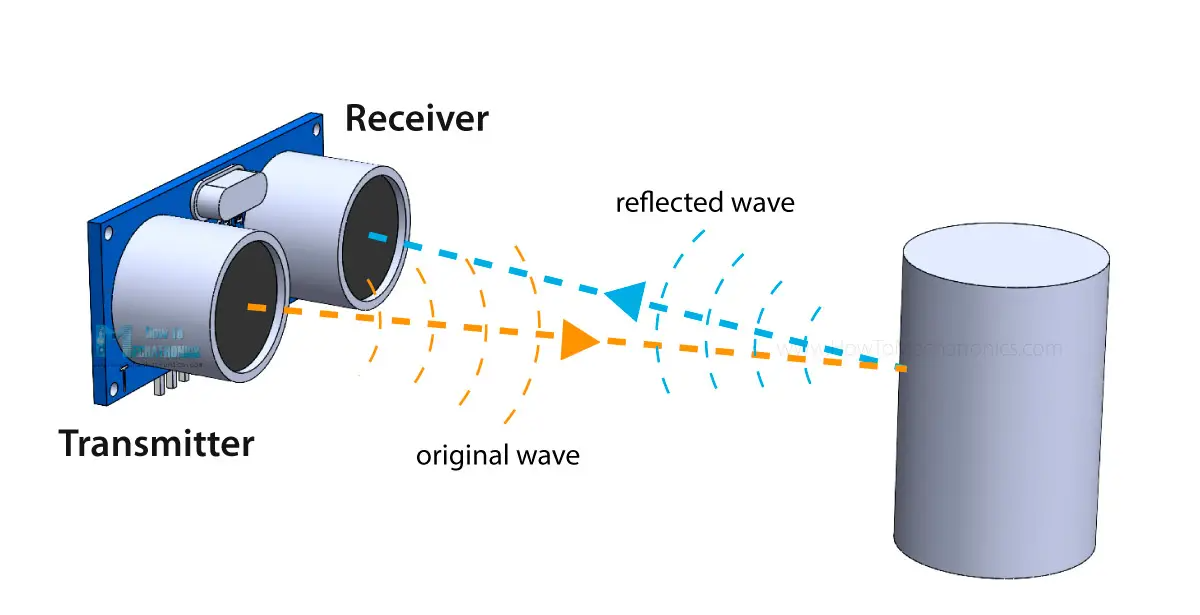
\includegraphics[width=0.74\textwidth]{images/literature/ultrasonic_principle.png}
            \caption{Illustration of the HC-SR04 ultrasonic sensor's working principle (Concept from~\cite{howtomechatronics_ultrasonic}).}
            \label{fig:ultrasonic_principle}
        \end{figure}
    \item \textbf{Infrared Proximity and Cliff Sensors:} Used for short-range detection and crucially as ``cliff sensors'' (typically under the robot) to detect drops like stairs by measuring reflected \hyperref[term:ir]{IR} light.
    \item \textbf{Optical Limit Switches (Bump Sensors):} Physical contact sensors, usually in the robot's bumper, that activate upon collision, providing a definitive, albeit reactive, obstacle signal.
    \item \textbf{3D Depth Sensors:} Provide a richer 3D understanding of surroundings. Examples include stereo cameras (using two cameras for depth via parallax) and structured light sensors (projecting light patterns). They help detect complex or low-lying obstacles.
    \item \textbf{\hyperref[term:lidar]{LiDAR} for Obstacle Detection:} While key for \hyperref[term:slam]{SLAM}, \hyperref[term:lidar]{LiDAR} (e.g., \hyperref[term:rplidar]{RPLidar} models) also directly provides precise distance measurements in a point cloud, useful for immediate obstacle detection.
    \item \textbf{Cameras for Obstacle Detection:} Similarly, cameras, vital for \hyperref[term:vslam]{vSLAM}, can also be used directly for obstacle detection via computer vision algorithms that identify objects in the robot's path.
\end{itemize}

\subsection*{Cleaning Mechanisms}
Robots use different tools to clean:
\begin{itemize}
    \item \textbf{Vacuum Suction:} This is the most common way. A fan or motor creates suction to pull dust and dirt into a container. How well this works depends on the motor's power, how the airflow is designed, and the shape of the vacuum nozzle.
    \item \textbf{Rotating Brushes:} These are often used with vacuuming. Main brushes (roller brushes) help loosen dirt from carpets or sweep hard floors. Side brushes stick out from the robot's sides to sweep dirt from edges and corners into the main cleaning area.
    \item \textbf{Mopping Systems:} Some robots can also mop. Simple ones might just drag a wet or dry cloth. More advanced ones have water tanks, control how much water is used, and sometimes have mop pads that vibrate or scrub.
\end{itemize}

\subsection*{Control Systems}
The part of the robot that controls everything can be different:
\begin{itemize}
    \item \textbf{Microcontroller-Based Logic:} Simpler robots often use small computer chips called microcontrollers (like Arduino or ESP32, or the Raspberry Pi Pico W~\cite{PicoWDatasheet} in this project). These are programmed with specific instructions for moving, using sensors, and cleaning. They are cheap and good for basic tasks.
    \item \textbf{Single-Board Computers:} More powerful options like the Raspberry Pi (the full version, not Pico) can run full computer operating systems (like Linux). This allows them to use more complex software, making them suitable for computationally intensive tasks like \hyperref[term:slam]{SLAM} or running frameworks like \hyperref[term:ros]{ROS}.
    \item \textbf{Robot Operating System:} \hyperref[term:ros]{ROS} is a set of software tools and libraries for building robot applications~\cite{ROSWiki}. It helps with tasks like navigation, understanding sensor data, and controlling robot parts. Using \hyperref[term:ros]{ROS} usually needs a more powerful processor, like those in \hyperref[term:sbc]{SBC}s.
\end{itemize}

\subsection*{Power Management}
Robots that move on their own need a battery:
\begin{itemize}
    \item \textbf{Rechargeable Batteries:} These are standard. Older robots used NiCd or NiMH batteries.
    \item \textbf{Lithium-ion Batteries:} These are now the most popular because they store more energy in a smaller and lighter battery, last longer, and don't have the ``memory effect'' that older batteries did.
    \item \textbf{Automatic Recharging:} Many store-bought robots can automatically go back to a charging station when their battery is low. Some can even continue cleaning from where they stopped after recharging.
\end{itemize}
How these different technologies are used together determines what a cleaning robot can do, how well it works, and how much it costs. This project will choose carefully from these options to meet its specific goals.

\section{Analysis of Existing Designs}
\label{sec:analysis_existing_lit}
To help design the prototype for this project, I looked at several existing cleaning robot designs. This included simple non-commercial or custom-built projects, which are often easy and cheap to build, and more advanced commercial robots, which show high-end features and performance.

\subsection{Non-Commercial / Custom-Built Designs}
\label{subsec:non_commercial_designs_lit}
Non-commercial projects give good ideas on how to get basic functions working with few resources and common parts. They often show smart solutions and prove that core robot tasks can be done using common microcontrollers and sensors.
\subsubsection{Design 1: Ultimate Floor Cleaning Robot (Version 2.0)~\cite{ref1_agrawal2020ultimate}}
This project by Saiyam Agrawal is a robot that can mop and move around on its own in a basic way.
\begin{figure}[htbp]
    \centering
    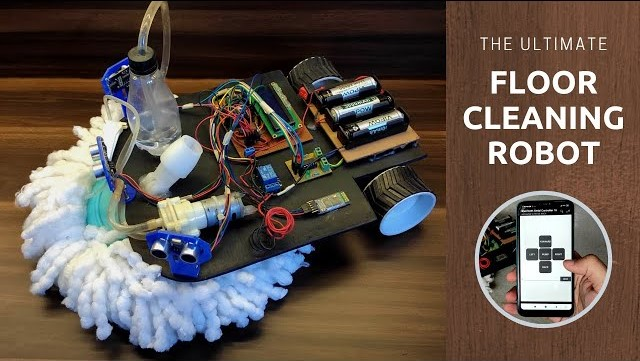
\includegraphics[width=0.75\textwidth, keepaspectratio]{images/literature/lit_ultimate_cleaning.jpg}
    \caption{Thumbnail of The Ultimate Floor Cleaning Robot (Version 2.0)~\cite{ref1_agrawal2020ultimate}.}
    \label{fig:thumbnail_ultimate_lit}
\end{figure}

\textbf{Key Features \& Analysis:}
\begin{itemize}
    \item \textbf{Navigation:} It uses three \hyperref[term:hcsr04]{HC-SR04} sensors (front, left, right) to see obstacles. An Arduino Nano controls it. The robot moves backward and turns based on what the sensors see. Using three sensors helps it see more around it than just one sensor. However, the creator mentions that its movement plan can have trouble in tricky spots like corners. This shows that simply reacting to what's nearby without a map can be difficult.
    \item \textbf{Cleaning:} It has a fixed mop. Water drips onto the mop from a bottle through a medical drip valve. This is a simple and cheap way to mop without needing motors for the mop. But, a problem noted is that the mop gets heavy when wet, which can make the wheels slip and affect how the robot moves.
    \item \textbf{Control:} It can be controlled manually with a smartphone app using Bluetooth (HC-05 module). This makes it user-friendly.
    \item \textbf{Power:} It uses three 18650 \hyperref[term:liion]{Li-ion} batteries connected together for 12V power. This shows that \hyperref[term:liion]{Li-ion} batteries are chosen because they are light.
    \item \textbf{Lessons for this Thesis:} This design shows it's possible to use several sensors and a cleaning tool with a simple microcontroller like an Arduino. The problems with complex navigation and the wet mop's weight affecting movement are important things to think about for the proposed robot's design and how weight is spread.
\end{itemize}
\subsubsection{Design 2: Arduino-Based Smart Vacuum Cleaner Robot~\cite{ref2_rizwan2021arduino}}
This project by ``Rizwan's Ideas'' is about making a vacuuming robot mostly from recycled items.
\begin{figure}[htbp]
    \centering
    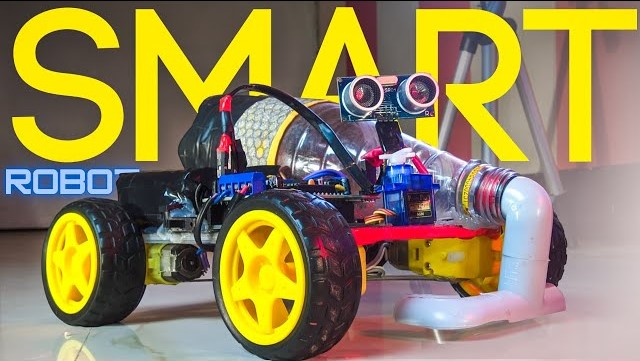
\includegraphics[width=0.75\textwidth, keepaspectratio]{images/literature/lit_arduino_vacuum.jpg}
    \caption{Thumbnail of Arduino based Smart Vacuum Cleaner Robot~\cite{ref2_rizwan2021arduino}.}
    \label{fig:thumbnail_arduino_lit}
\end{figure}

\textbf{Key Features \& Analysis:}
\begin{itemize}
    \item \textbf{Building Materials:} It focuses on saving money by using a plastic bottle and cardboard for the robot's body.
    \item \textbf{Navigation:} An Arduino Uno controls four \hyperref[term:dc]{DC} motors using a motor shield. One \hyperref[term:hcsr04]{HC-SR04} ultrasonic sensor is put on a servo motor. This lets the sensor turn and scan for obstacles. Scanning can help see a wider area than a fixed sensor, but it makes the robot more complex mechanically and takes time to scan.
    \item \textbf{Cleaning:} The vacuum system is very basic, using a small 6V fan motor inside the plastic bottle. The creator says the suction is not very strong. This is a common issue in very cheap custom-built vacuum designs that don't use special high-speed fans.
    \item \textbf{Lessons for this Thesis:} This design shows how to be creative with materials. The sensor on a servo is an interesting way to make one sensor see more, but it has its own difficulties. The weak suction shows that choosing a good fan and designing good airflow is important for vacuuming. Using four motors might be for better movement or just because those parts were available.
\end{itemize}
\subsubsection{Design 3: Self-Navigating Vacuum Cleaner (Video by SciNix)~\cite{ref4_scinix2023selfnav}}
This project by SciNix shows a more advanced custom-built robot that uses the \hyperref[term:ros]{ROS}.
\begin{figure}[htbp]
    \centering
    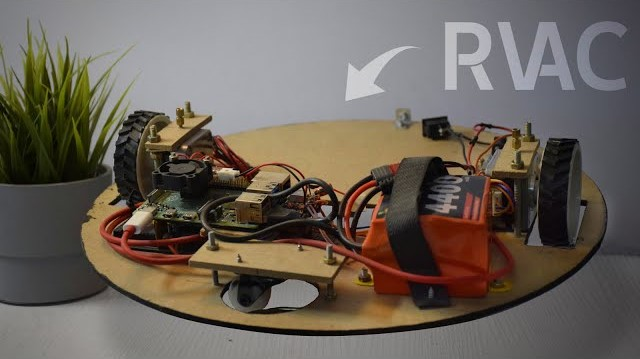
\includegraphics[width=0.75\textwidth, keepaspectratio]{images/literature/lit_selfnav_vacuum.jpg}
    \caption{Thumbnail of Self-Navigating Vacuum Cleaner~\cite{ref4_scinix2023selfnav}.}
    \label{fig:thumbnail_selfnav_lit}
\end{figure}

\textbf{Key Features \& Analysis:}
\begin{itemize}
    \item \textbf{Control System:} It uses a Raspberry Pi 4 to run the \hyperref[term:ros]{ROS} Navigation Stack. This software handles moving around on its own and planning paths based on maps made beforehand. An Arduino Mega is used as a simpler controller for the stepper motors.
    \item \textbf{Movement:} It uses stepper motors for very
    precise movement. This might mean it doesn't need wheel encoders if the steps are counted correctly, but it could have problems with wheels slipping if not handled well.
    \item \textbf{Navigation:} Using \hyperref[term:ros]{ROS} is a big step up in software difficulty compared to typical Arduino projects. It allows for much smarter path planning (for example, using global and local planners to decide where to go).
    \item \textbf{Lessons for this Thesis:} This design shows a way to make a custom-built robot much more autonomous. Even though this thesis's project uses a Raspberry Pi Pico W (which is a microcontroller, not a full computer like the Pi 4) and doesn't plan to use \hyperref[term:ros]{ROS} at first, the SciNix project shows that more powerful processors and software can greatly improve how a robot moves around. It reminds us to design the current robot so it can be upgraded in the future.
\end{itemize}
\subsubsection{Design 4: Advanced Cleaning Robot Analysis (Video by Sabin Civil Engineering)~\cite{ref3_sabin2022amazing}}
This YouTube video provides an overview of the technologies and evolutionary stages of advanced cleaning robots, rather than detailing a single custom-built project. It discusses how these robots integrate various components and intelligence levels to achieve autonomous cleaning.
\begin{figure}[htbp]
    \centering
    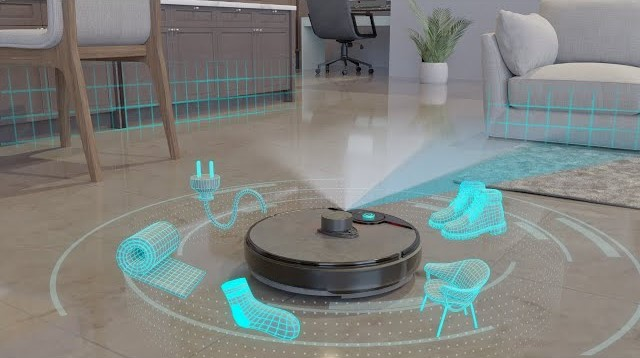
\includegraphics[width=0.75\textwidth, keepaspectratio]{images/literature/lit_sabin_analysis.jpg}
    \caption{Thumbnail of The Amazing Engineering behind Cleaning Robots~\cite{ref3_sabin2022amazing}.}
    \label{fig:thumbnail_amazing_lit}
\end{figure}

\textbf{Key Ideas Discussed \& Analysis:}
\begin{itemize}
    \item \textbf{Core Cleaning and Locomotion:} The foundation includes a vacuum pump for debris collection, driven by tractor wheels and a caster wheel for movement. To enhance cleaning width beyond the vacuum pump's direct opening, side brushes and a roller brush are employed to guide debris towards the suction area, improving efficiency, especially in corners. Some designs incorporate mopping attachments with controlled water flow for removing tough stains simultaneously with vacuuming.
    \item \textbf{Evolution of Obstacle Handling and Navigation:}
        \begin{itemize}
            \item \textbf{Initial Reactive Obstacle Detection:} To address the issue of robots getting stuck, optical limit switches (bump sensors) are added to the front bumper. When an object is hit, these switches signal a smart controller.
            \item \textbf{Basic Turning Maneuvers:} The controller then manages individual wheel speeds, enabling the robot to turn (e.g., by rotating wheels in opposite directions) after a collision. However, this random path is inefficient.
            \item \textbf{Improving Path Efficiency:} For more systematic coverage, robots need to make accurate turns (e.g., right angles) and control travel distance to avoid excessive overlap. This leads to the integration of a gyroscope sensor for precise angular turns and wheel encoders to measure distance by counting wheel rotations.
            \item \textbf{Advanced Obstacle Differentiation and Mapping:} A limitation of simpler sensor setups (bump, gyro, encoders) is the inability to differentiate between types of obstacles (e.g., a wall versus a chair leg), potentially leaving areas uncleaned. The introduction of a \hyperref[term:lidar]{LiDAR} sensor addresses this by emitting lasers and creating a 2D map of the room as it rotates. This map allows the robot to distinguish objects and follow more efficient cleaning paths.
            \item \textbf{Cliff and Drop Detection:} Standard 2D \hyperref[term:lidar]{LiDAR} may not detect drops like staircases. To prevent falls, optical proximity sensors (typically \hyperref[term:ir]{IR} emitters and detectors) are placed at the robot's edge. These measure reflected light, and a sudden loss of reflection signals a drop, prompting the controller to stop and redirect the robot.
            \item \textbf{Detecting Small or Low-Lying Obstacles:} 2D \hyperref[term:lidar]{LiDAR} can also miss small or flat obstacles on the floor, such as wires, clothes, or pet waste. To address this, a camera, often combined with an inbuilt 3D depth sensor, is added to the front. This system maps the immediate frontal region in 3D, enabling precise detection and avoidance of such objects.
            \item \textbf{Sensor Fusion:} The video highlights the Sensor Fusion technique, which involves combining data from multiple sensor types (e.g., \hyperref[term:lidar]{LiDAR} and camera systems) to achieve more accurate and robust environmental perception and cleaning paths.
        \end{itemize}
    \item \textbf{User Interaction and Convenience Features:} Advanced robots often include mobile application integration for features like setting go/no-go zones, scheduling cleaning sessions, and targeting specific areas for cleaning.
    \item \textbf{Physical Capabilities:} The ability to climb small heights, such as door ramps (up to approximately 2 cm), is noted as a physical capability of some robots.
    \item \textbf{Power Management:} Automatic recharging, where the robot autonomously returns to its charging dock when the battery is low, is a key convenience feature.
\end{itemize}
\textbf{Lessons for this Thesis:} This overview of advanced robot features underscores the complexity and multi-layered sensing involved in achieving high levels of autonomy and cleaning effectiveness. It clearly illustrates the progression from basic reactive behaviors to sophisticated mapping, navigation, and object recognition capabilities. For this project, which aims for a cost-effective prototype with core functionalities, this analysis provides a valuable benchmark and highlights potential pathways for future enhancements. While full \hyperref[term:slam]{SLAM} with sensor fusion is beyond the current scope, understanding the role of individual sensors (like ultrasonic for basic detection, potential for \hyperref[term:ir]{IR} cliff sensors, or even a simple camera in the future) and the importance of intelligent obstacle response logic is highly relevant. The discussion on efficient path coverage, even with simpler sensors, also informs the design of the autonomous navigation algorithm for this project.
\subsection{Commercial Cleaning Robot Designs}
\label{subsec:commercial_designs_lit}
Store-bought robots show what is possible in terms of performance, features, and ease of use. Looking at them helps us understand what people expect from these robots and see how advanced technologies are used.

\subsubsection{Product 1: iRobot Roomba 980~\cite{ref5_irobot980, ref6_techchap_roomba980}}
The iRobot Roomba 980 is a well-known high-quality robot vacuum cleaner, famous for its smart features and good cleaning.
\begin{figure}[htbp]
    \centering
    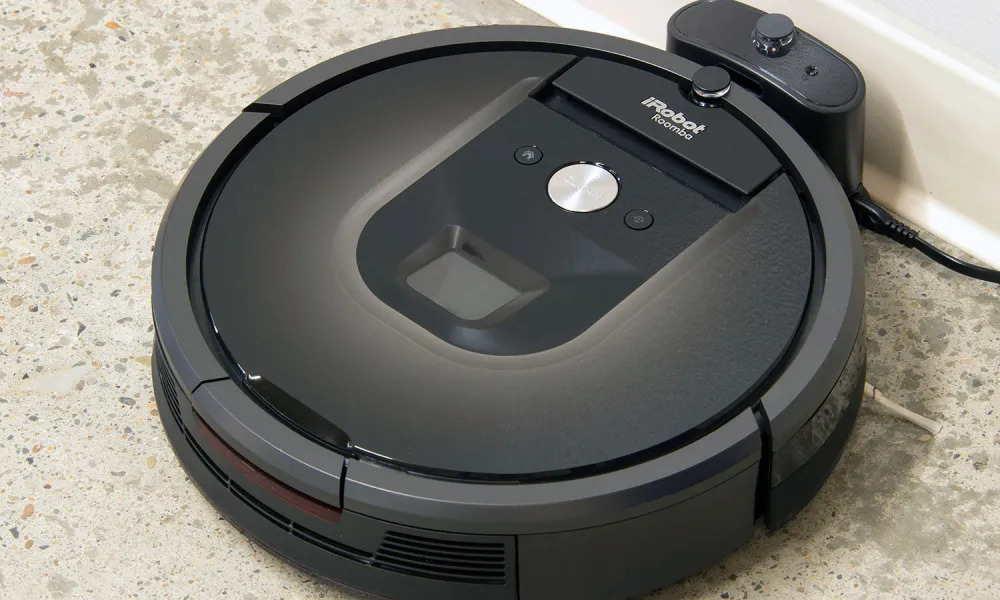
\includegraphics[width=0.75\textwidth, keepaspectratio]{images/literature/roomba_980.jpg}
    \caption{Photo of iRobot Roomba 980~\cite{ref5_irobot980}.}
    \label{fig:roomba980_lit}
\end{figure}

\textbf{Key Features \& Detailed Analysis:}
\begin{itemize}
    \item \textbf{Navigation (\hyperref[term:vslam]{vSLAM}):} The Roomba 980 uses an advanced navigation system with a camera. The camera, facing upwards, constantly takes pictures of the room, finding unique visual points (like patterns on the ceiling, edges of furniture, and walls). By tracking these points from picture to picture and combining this with its own movement information (often from wheel sensors and an \hyperref[term:imu]{IMU}), the robot builds a map of the room and knows where it is on that map. This \hyperref[term:vslam]{vSLAM} ability allows it to clean in an organized and efficient way (like in straight lines, one room at a time) instead of just bouncing around randomly like simpler robots. It can usually clean a whole floor of a house and remember where it has already cleaned.
    \item \textbf{Adaptive Cleaning Technologies:}
        \begin{itemize}
            \item \textbf{PowerBoost:} This feature automatically makes the vacuum stronger when the robot senses it's on a carpet. Sensors (maybe optical or by noticing if the motors are working harder) detect the carpet. This makes the vacuum more powerful to pick up dirt stuck in the carpet. On hard floors, it uses normal suction to save battery.
            \item \textbf{Dirt Detect™ Series II Technology:} The Roomba 980 uses special sensors (optical and acoustic) to find areas with more dirt. When these sensors find a lot of dirt, the robot changes how it cleans that spot. It might go over the area several times or use a special pattern until it thinks the area is clean. This makes sure dirtier spots get cleaned better.
        \end{itemize}
    \item \textbf{Other Important Features:}
        \begin{itemize}
            \item \textbf{Edge-Cleaning Brush:} A spinning side brush sweeps dirt from along walls, under cabinets, and around furniture legs. It pushes the dirt into the path of the main brushes and vacuum.
            \item \textbf{Wi-Fi and iRobot HOME App:} The robot connects to the home Wi-Fi. This lets users control and check on it from far away using a smartphone app. The app usually lets you start, stop, or pause cleaning; set up regular cleaning times; change cleaning settings (like how many times to go over an area); see maps of where the robot cleaned; and get messages.
            \item \textbf{Automatic Recharging and Resuming:} If the battery gets low while cleaning, the Roomba 980 is designed to go back to its charging station by itself. After it has recharged enough, it can start cleaning again from where it stopped. This is helpful for cleaning large areas without needing someone to do anything.
        \end{itemize}
    \item \textbf{Market Importance:} When the Roomba 980 came out, it really improved what people expected from robot vacuums. It showed how \hyperref[term:vslam]{vSLAM} could be used for good navigation in homes and introduced smart features like changing suction power and finding very dirty spots. These features helped iRobot become a leading company and changed what consumers thought a ``smart'' vacuum cleaner should do, especially regarding how well it cleans on its own, how smart it is, and how easy it is to use with an app.
\end{itemize}
\subsubsection{Product 2: Xiaomi Robot Vacuum X20 Plus~\cite{ref7_xiaomiX20plus, ref8_wester_xiaomiX20plus}}
The Xiaomi Robot Vacuum X20 Plus is an example of a robot that includes very new features, especially for navigation and taking care of itself. It often sells for a lower price than other top brands, making it a strong competitor.
\begin{figure}[htbp]
    \centering
    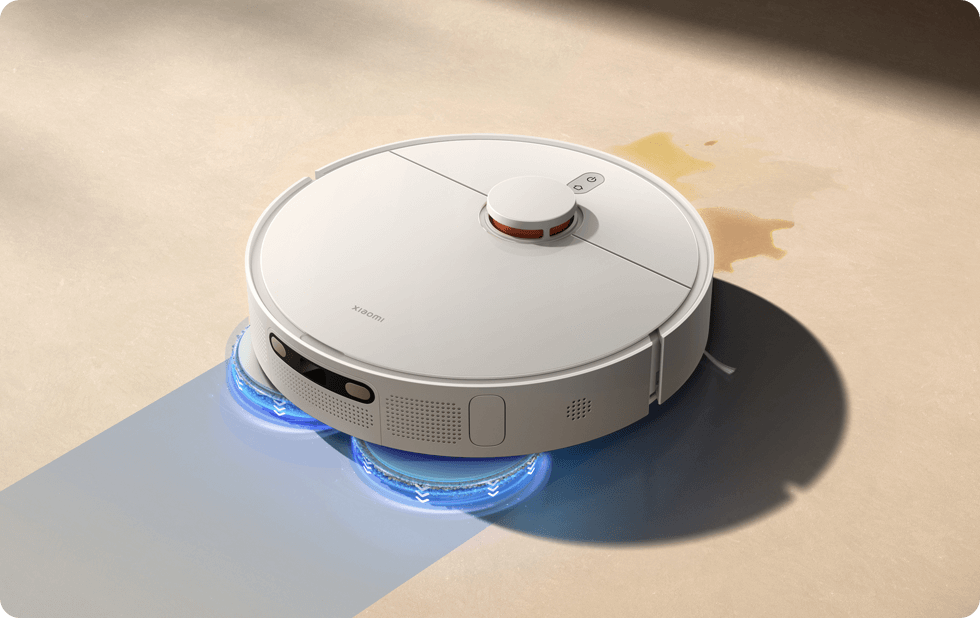
\includegraphics[width=0.75\textwidth, keepaspectratio]{images/literature/xiaomi_x20.png}
    \caption{Photo of Xiaomi Robot Vacuum X20 Plus~\cite{ref7_xiaomiX20plus}.}
    \label{fig:xiaomiX20_lit}
\end{figure}
\textbf{Key Features \& Detailed Analysis:}
\begin{itemize}
    \item \textbf{Navigation (\hyperref[term:lds]{LDS} / \hyperref[term:lidar]{LiDAR}):} The X20 Plus uses an \hyperref[term:lds]{LDS} navigation system, which is a type of \hyperref[term:lidar]{LiDAR}. A laser turret on top of the robot spins quickly, sending out laser beams and measuring the reflected light. This creates a very accurate 360-degree map of the room in real time. This technology allows for very precise distance measurements and map making. This helps the robot plan efficient and orderly cleaning paths, move around complex furniture, and work well even in dim light where cameras might have trouble. The maps it creates can often be seen in an app. Users can use these maps to set up virtual walls (to keep the robot out of certain areas), no-go zones, or choose specific spots for the robot to clean.
    \item \textbf{Hybrid Cleaning (Vacuuming and Mopping):} This model can do two jobs: it has strong vacuum suction and an attached mopping system. The vacuum system usually has high suction power (measured in Pascals) to pick up dust, hair, and bigger pieces of dirt. The mopping system might have a water tank and a microfiber mop pad. Advanced mopping features can include electronic control of water flow to change how damp the mop is, and sometimes special mopping movements (like a Y-shape scrubbing motion) to clean stains better.
    \item \textbf{Comprehensive Self-Maintenance Station:} A major feature of the X20 Plus (and similar high-end robots) is its all-in-one station that automatically empties the dustbin and washes the mop. This greatly reduces how much users have to do manually:
        \begin{itemize}
            \item \textbf{Automatic Dustbin Emptying:} After cleaning, the robot goes to its dock. The station then uses strong suction to empty the robot's small dustbin into a much larger dust bag or container in the station. This means the robot can clean for weeks before the user needs to empty the station's container.
            \item \textbf{Automatic Mop Washing:} The station can clean the robot's mop pads. This might involve parts like spinning scrubbers, fresh water sprays to wash the pads, and a system to collect the dirty water.
            \item \textbf{Automatic Mop Drying:} After washing, the station often uses warm air to dry the mop pads. This stops mold and smells from growing and makes sure the mop is clean for the next use.
        \end{itemize}
    \item \textbf{Market Importance:} The Xiaomi X20 Plus and similar robots show how quickly advanced features are becoming common and more affordable. The use of \hyperref[term:lidar]{LiDAR} for precise navigation and especially the smart self-maintenance stations solve big problems that users had with older robot vacuums (like having to empty the dustbin often and clean the mop by hand). This pushes the industry towards robots that are not just autonomous in cleaning, but also in their own upkeep, making them much more convenient and user-friendly.
\end{itemize}
These commercial examples demonstrate the sophisticated capabilities that are possible with advanced sensor suites, powerful processing, and refined algorithms. While this project aims for a more modest set of features due to cost and complexity constraints, understanding these high-end systems provides valuable context and inspiration for future development.

\section{Key Takeaways and Problem Statement}
\label{sec:takeaways_problem_lit}
Looking at both non-commercial projects and store-bought robots shows a wide and quickly changing world of cleaning robot technology. We can see a clear range:
\begin{itemize}
    \item On one side, non-commercial projects show that it's possible to build basic cleaning robots with cheap and easy-to-find parts. These projects are often simple and can be changed to fit specific needs. However, they often don't move around very well, clean as effectively, or work as independently as more advanced robots. They usually just react to what's around them, and their cleaning tools can be very basic.
    \item On the other side, high-end store-bought robots are very advanced. They have many smart sensors (like \hyperref[term:lidar]{LiDAR} and cameras), complex software (for \hyperref[term:slam]{SLAM} and AI-based path planning), powerful cleaning systems, and many automatic features, like charging themselves and emptying their own dustbins. But, these advanced features make them very expensive, so not everyone can afford them.
\end{itemize}
This review clearly shows a big gap in the market: there's a need for automated cleaning solutions that offer a good mix of features and affordability. Many people might want something better than basic custom-built kits but are not ready to pay for the most expensive commercial robots.

\textbf{Problem Statement:}
This bachelor thesis project aims to fill this gap by designing and building a smart cleaning robot prototype that carefully balances useful features, ease of use, and reasonable cost. The main goal is to create a system using parts that are easy to find, affordable, and have good support for typical homes, especially those with common floor types found in places like Egypt.
The core technical challenge this project addresses is achieving reliable and repeatable navigation on a budget. The main focus is therefore to implement \textbf{closed-loop motor control via wheel encoders}, moving beyond the unpredictable, timed-based movements common in simpler designs. This is complemented by \hyperref[term:ble]{BLE} remote control for manual operation. The system is built around a Raspberry Pi Pico W microcontroller, \hyperref[term:hcsr04]{HC-SR04} sensors for basic sensing, standard \hyperref[term:dc]{DC} motors, and a repurposed fan for an effective vacuum. While fully independent mapping and path planning (like \hyperref[term:slam]{SLAM}) are beyond the scope of this first prototype, this project aims to create a robust foundation for more advanced features. It seeks a middle ground between simplistic DIY kits and expensive commercial robots, with a modular design that creates a clear path for future development in affordable home robotics.
% --- NEW Chapter 3: Mechanical Design and Assembly ---
\chapter{Mechanical Design and Assembly}
\label{chap:mechanical_design_assembly}

\section{Introduction}
\label{sec:mech_intro}
This chapter details the mechanical design and physical construction of the Smart Cleaning Robot prototype. It covers the overall structural design, the \hyperref[term:cad]{CAD}-based development of individual components using SolidWorks, material considerations, and the assembly of the robot's chassis, the encoder-based drive system for precision tracking, and the integrated vacuum cleaning mechanism. The dimensions for the custom-designed parts in SolidWorks were determined based on the physical sizes of the selected electronic and mechanical components. A comprehensive Bill of Materials, including all components and associated costs, can be found in Appendix \ref{app:bom}.
The design prioritizes functionality, ease of assembly for a prototype, and component housing while also considering the challenges encountered during fabrication and iteration.
The overall dimensions of the assembled robot are approximately 35cm in diameter and 17cm in height (excluding the small wheel clearance). The fully assembled prototype has an approximate total weight of 2.65 kg.

\section{Mechanical Components Summary}
The key mechanical components providing the robot's structure and non-powered mobility are summarized in Table~\ref{tab:mechanical_components}. This table focuses only on the structural parts; the full list of electrical components is detailed in Chapter~\ref{chap:electrical_control_performance}, and a comprehensive Bill of Materials for all parts can be found in Appendix \ref{app:bom}.

\begingroup
\small % Make font smaller for the table content
\sloppy % Allow more flexible word spacing
\renewcommand{\arraystretch}{1.2} % Add some vertical padding
\begin{longtable}{|L{4.2cm}|p{2.3cm}|L{2.8cm}|L{3cm}|}
\caption{Mechanical Components List} \label{tab:mechanical_components} \\
\hline
\textbf{Component} & \textbf{Photo} & \textbf{Dimensions (cm)} & \textbf{Material} \\ \hline
\endfirsthead

\multicolumn{4}{c}%
{{\tablename\ \thetable\ -- \textit{Continued from previous page}}} \\
\hline
\textbf{Component} & \textbf{Photo} & \textbf{Dimensions (cm)} & \textbf{Material} \\ \hline
\endhead

\hline
\endlastfoot

% --- START OF MECHANICAL COMPONENTS ---

\textbf{Custom 3D-Printed Chassis} & 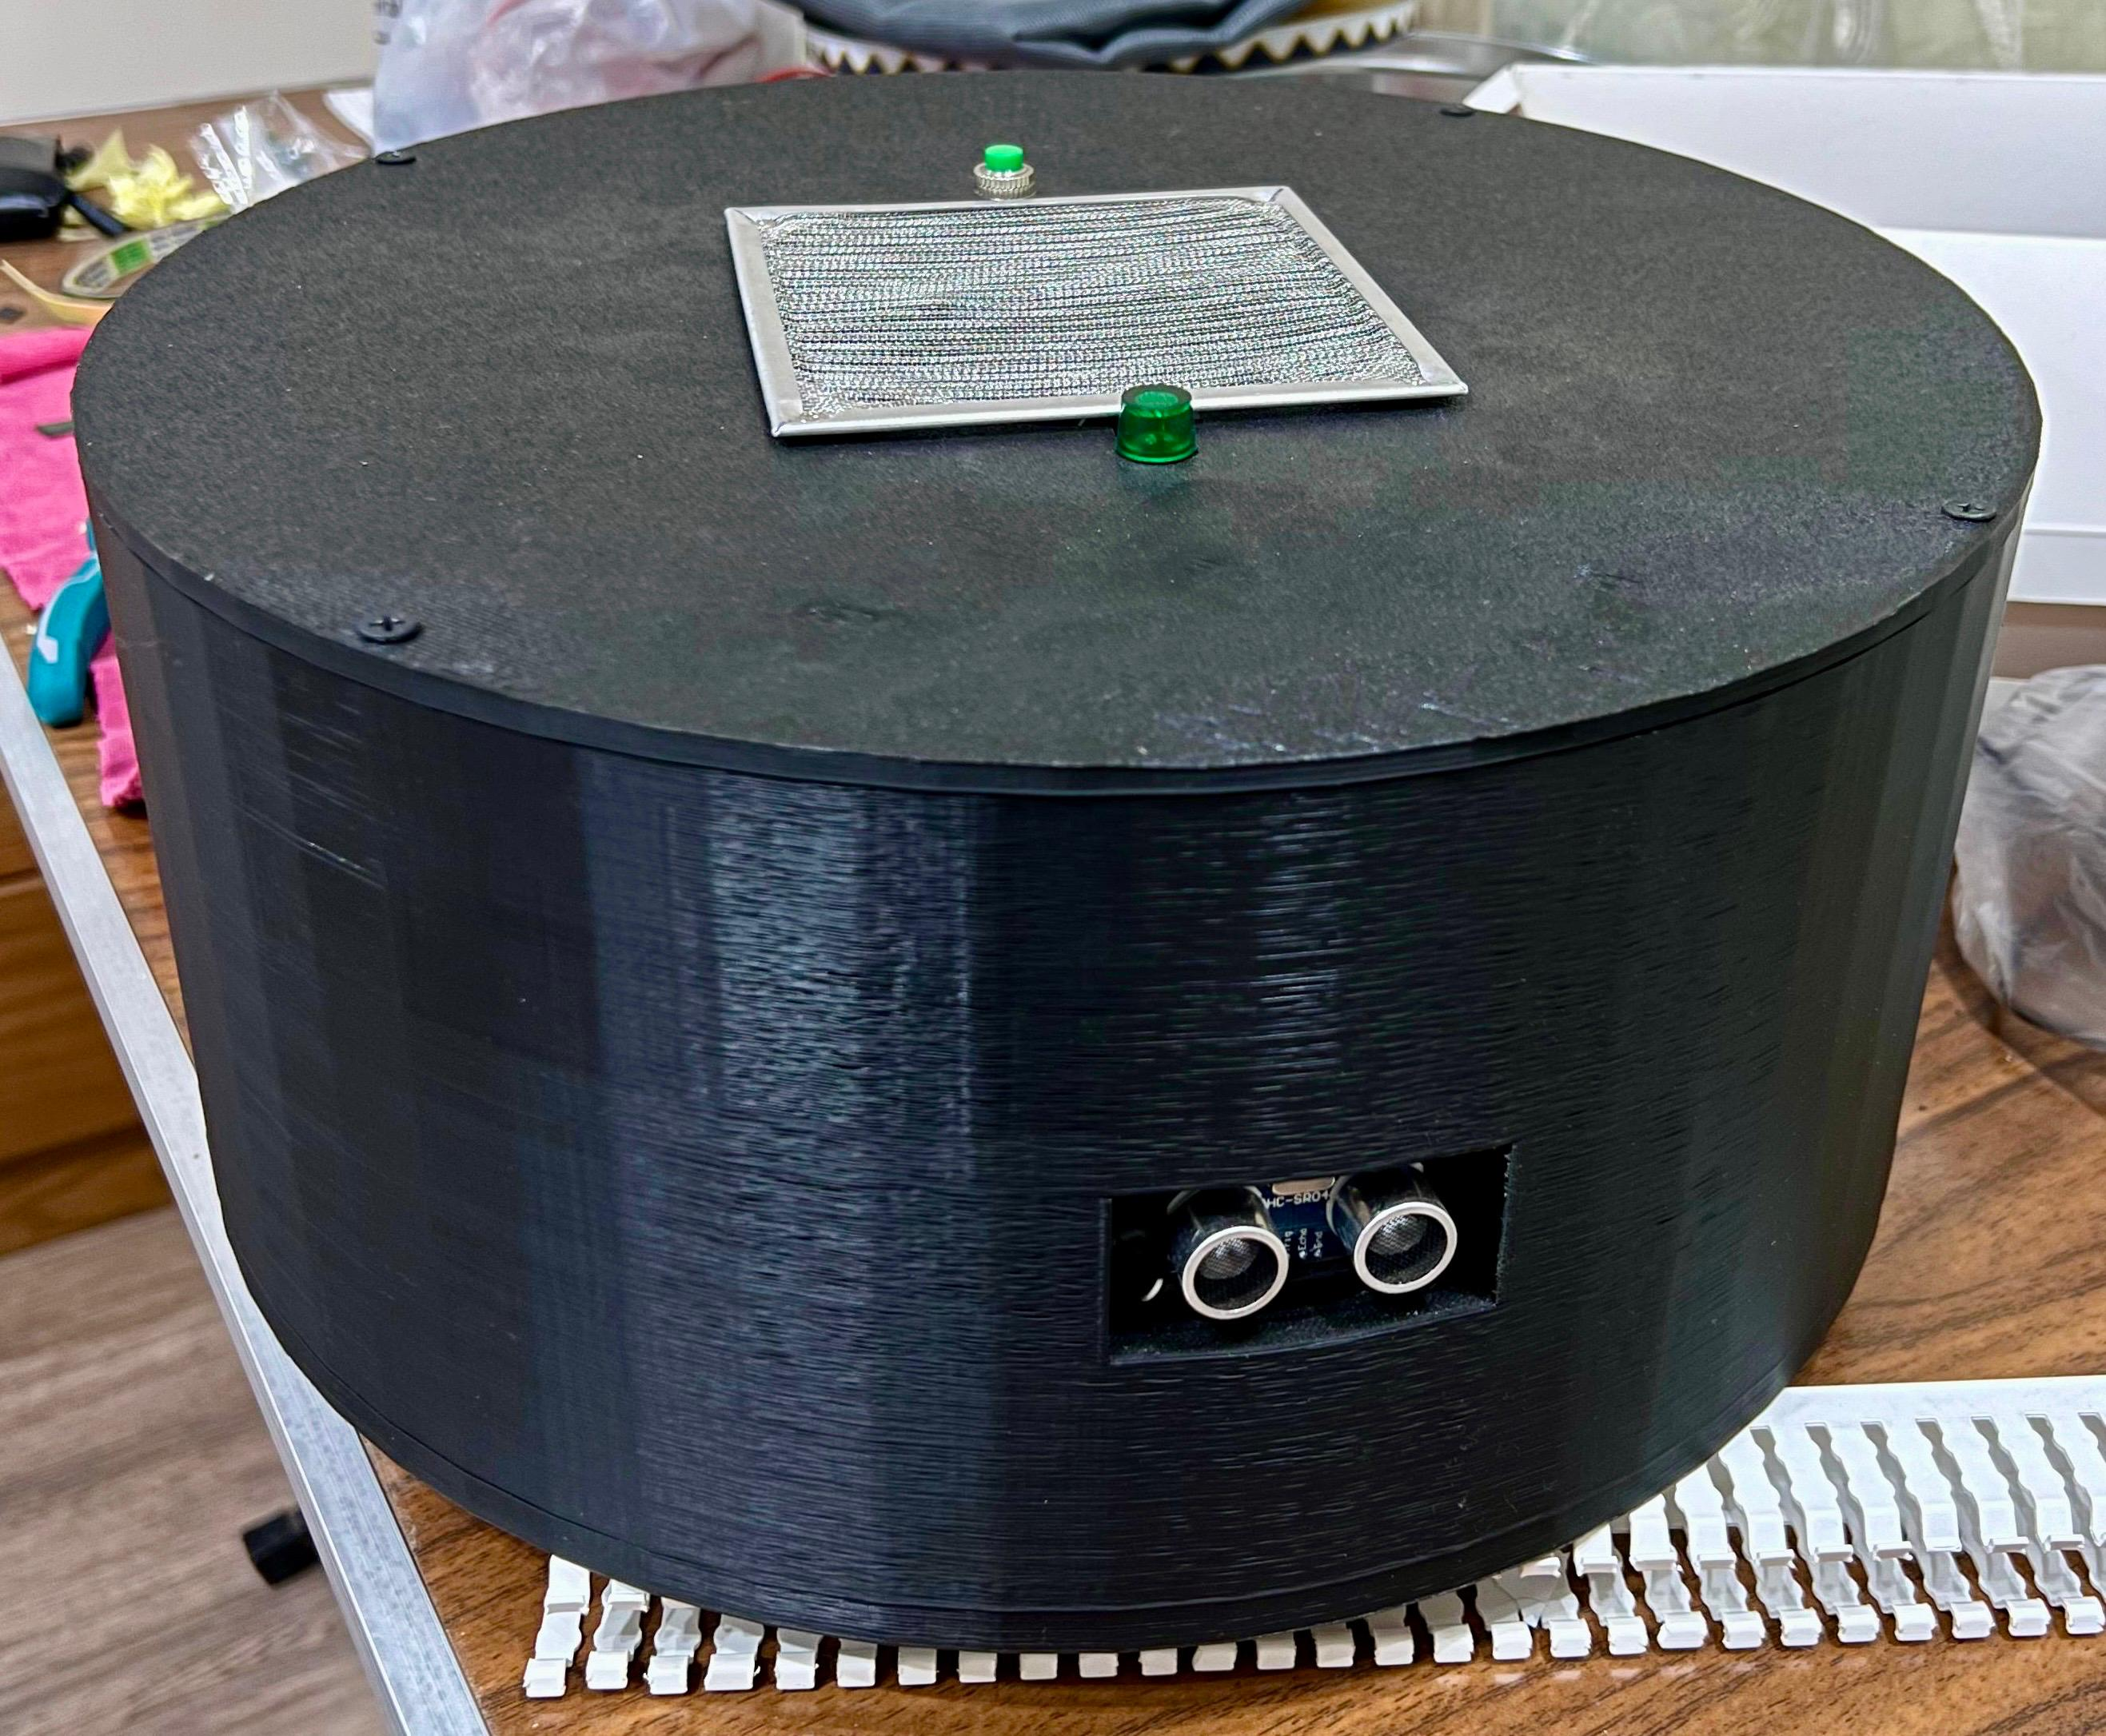
\includegraphics[width=0.9\linewidth, keepaspectratio]{images/photos/robot_assembled_iso.jpg} & $\varnothing \approx 35$, H $\approx 17$ & \hyperref[term:pla]{PLA}+ \\ \hline

\textbf{Custom 3D-Printed Debris Chamber} & 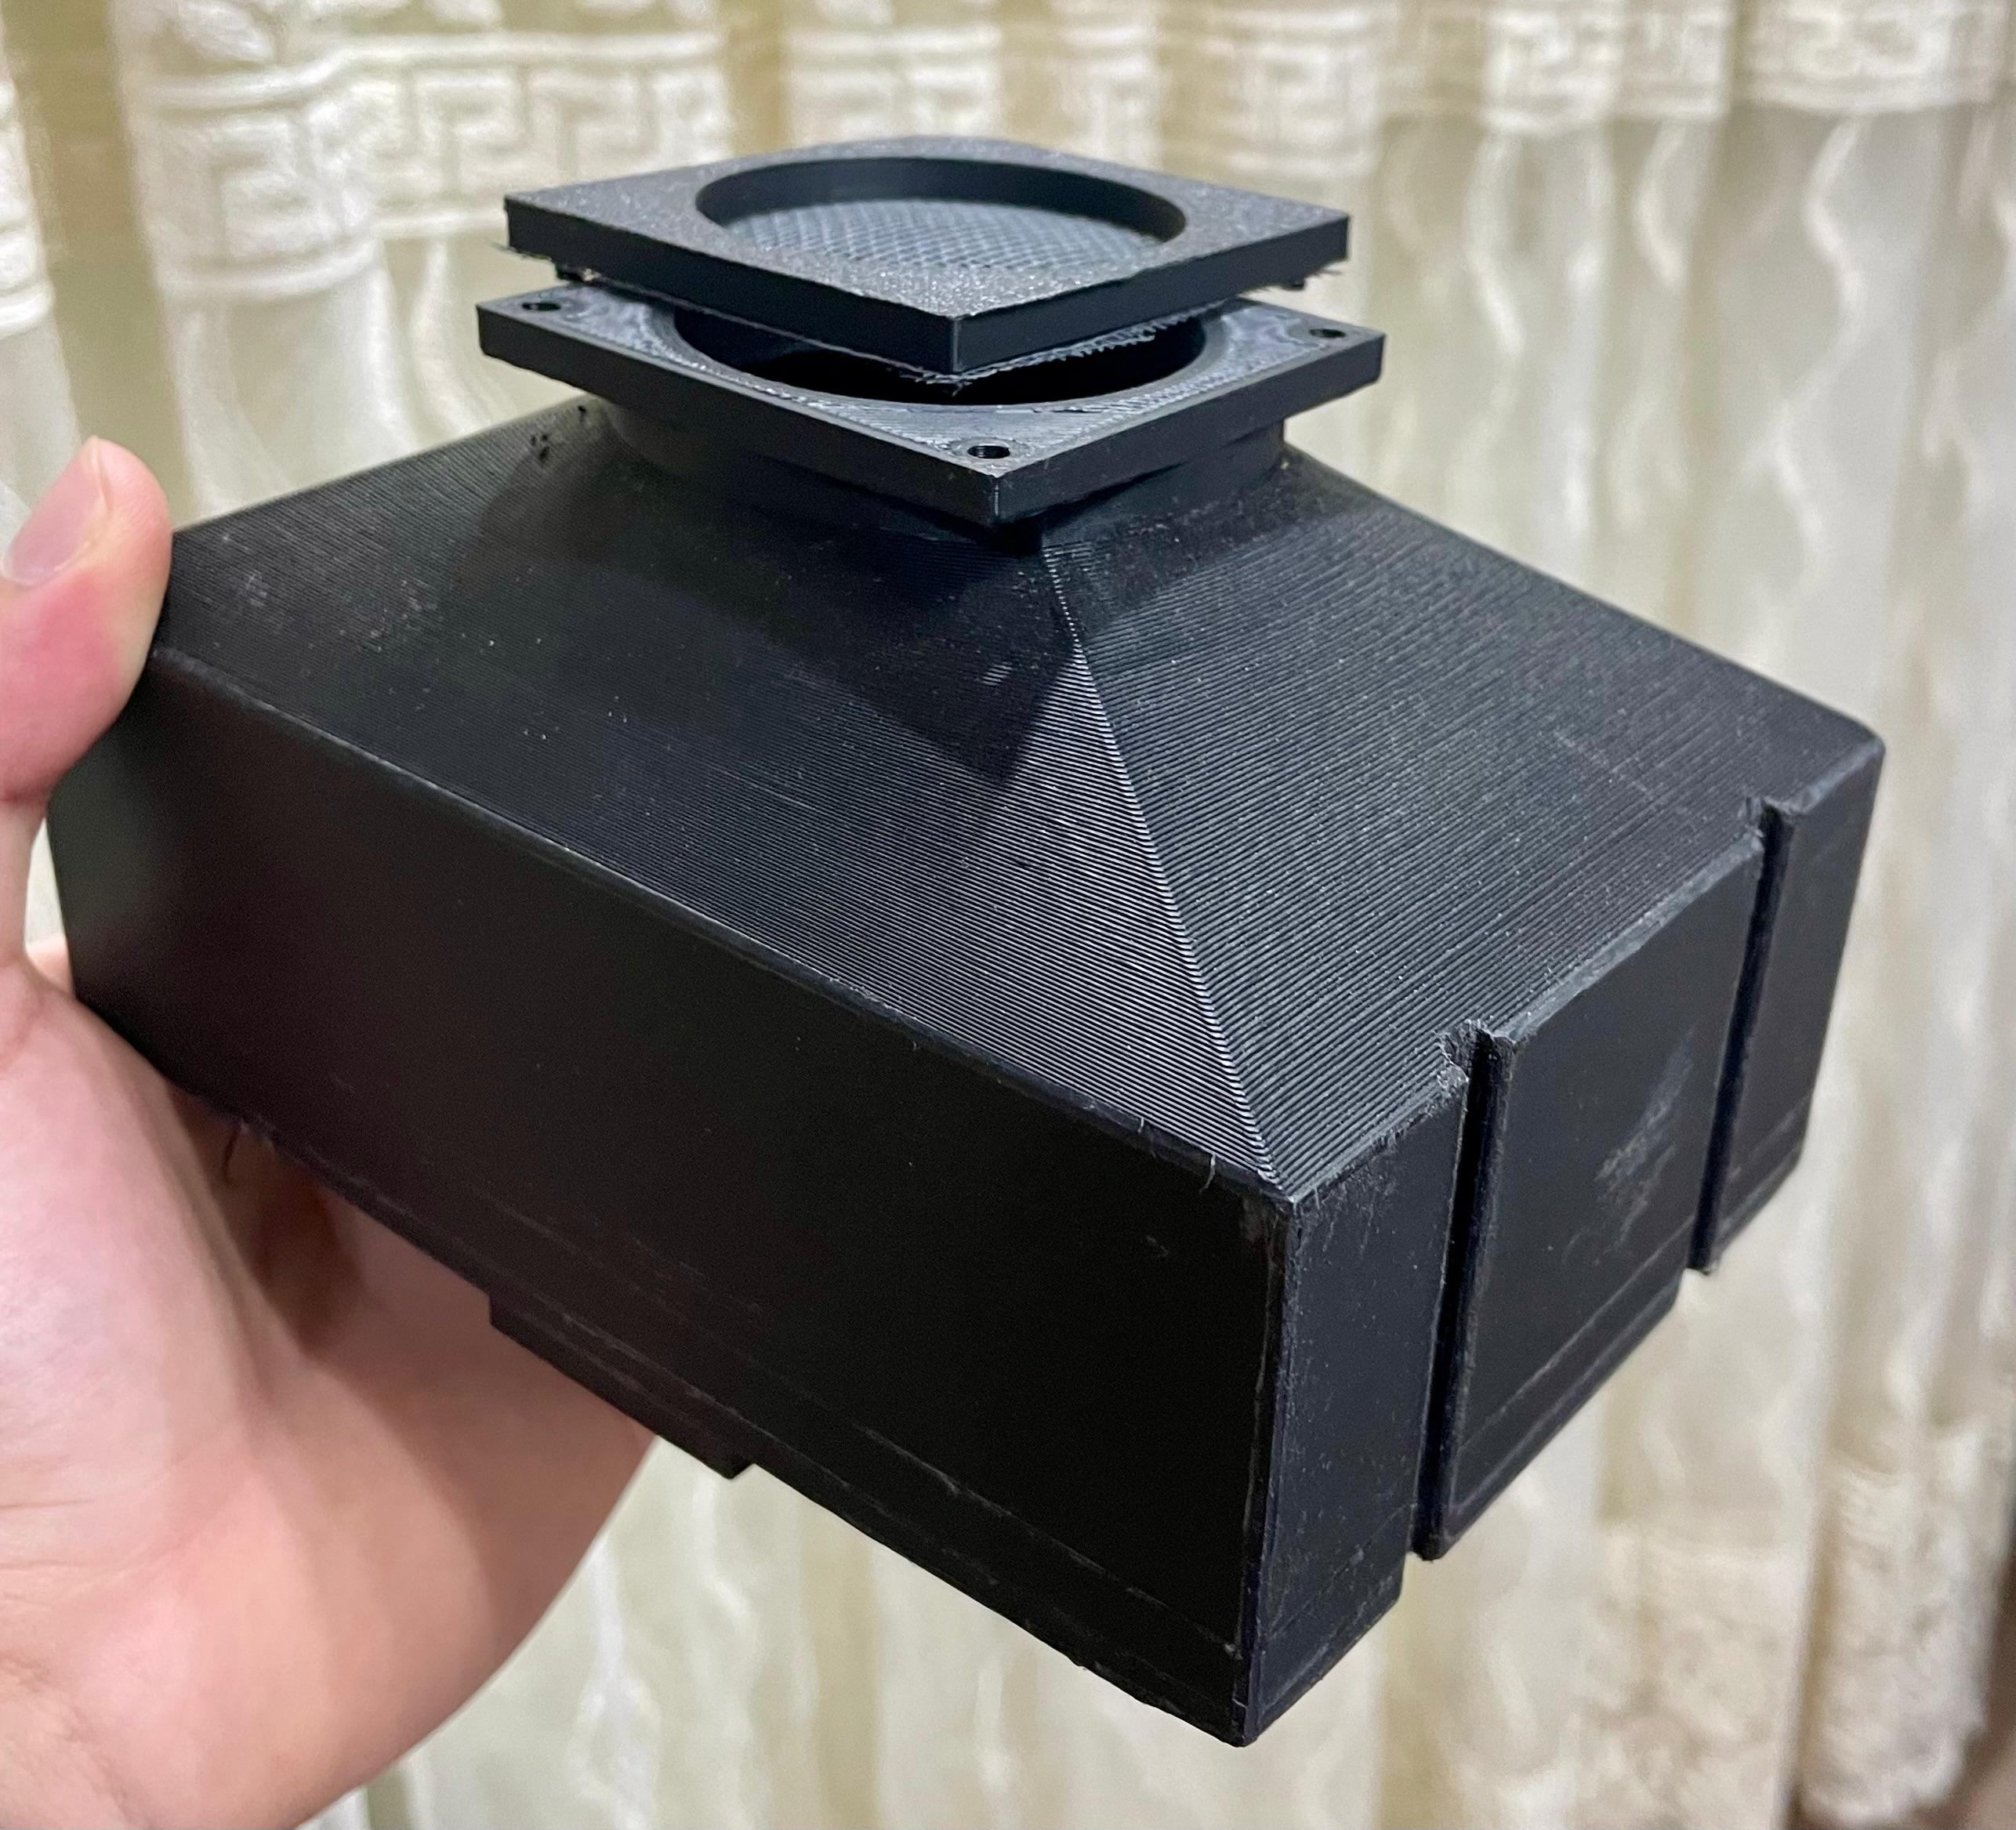
\includegraphics[width=0.9\linewidth, keepaspectratio]{images/photos/debris_chamber_photo.jpg} & WxLxH: 10.5$\times$16$\times$8 & \hyperref[term:pla]{PLA}+ \\ \hline

\href{https://www.maamoon.com/product-page/66mm-robot-smart-car-wheel-tyre}{\textbf{\textcolor{darkblue}{Robot Wheels}}} & 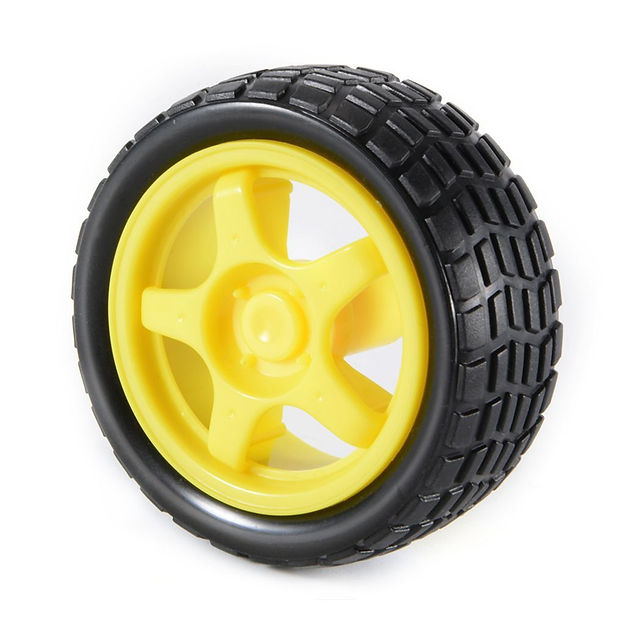
\includegraphics[width=0.9\linewidth, keepaspectratio]{images/components/wheel_66mm.jpg} & $\varnothing$: 6.6, W: 2.8 & Plastic Rim, Rubber Tyre \\ \hline

\href{https://www.ram-e-shop.com/shop/ro-wheel-caster-small-metal-caster-wheel-20-mm-robot-wheel-max-load-15kg-7010}{\textbf{\textcolor{darkblue}{Metal Caster Wheel}}} & 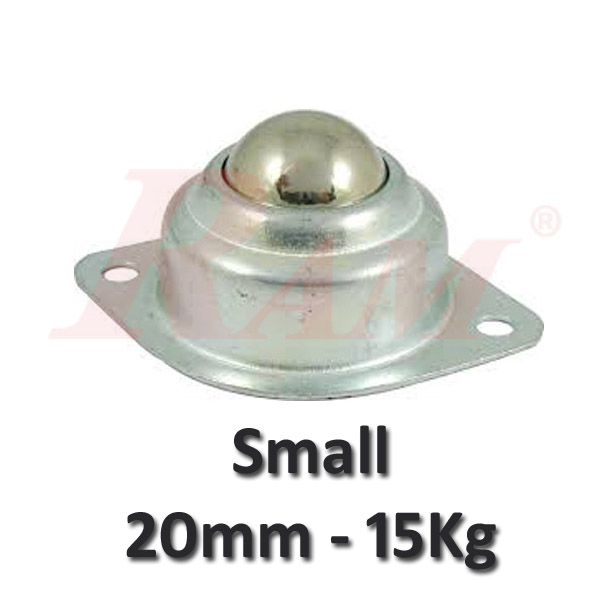
\includegraphics[width=0.9\linewidth, keepaspectratio]{images/components/caster_wheel.jpg} & Height: 2.0, Wheel $\varnothing$: 1.5 & Steel Body and Ball \\ \hline

\href{https://www.ram-e-shop.com/shop/spacer-screw-20mm-plastic-screw-shape-snap-in-rivet-pcb-spacer-20mm-5739}{\textbf{\textcolor{darkblue}{PCB Spacers (Snap-in Rivet)}}} & 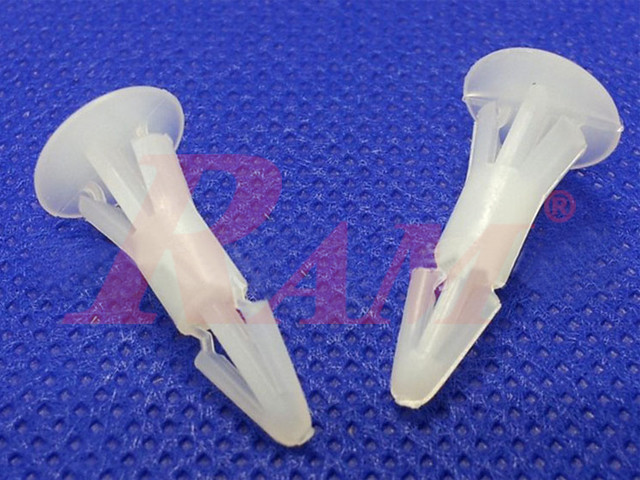
\includegraphics[width=0.9\linewidth, keepaspectratio]{images/components/pcb_spacer.jpg} & Length: 2.0 & Nylon \\ \hline

\href{https://www.ram-e-shop.com/shop/nail-3x05mm-bolt-m3x06-mm-100-screws-bag-6545}{\textbf{\textcolor{darkblue}{Bolts and Nuts (M3)}}} & 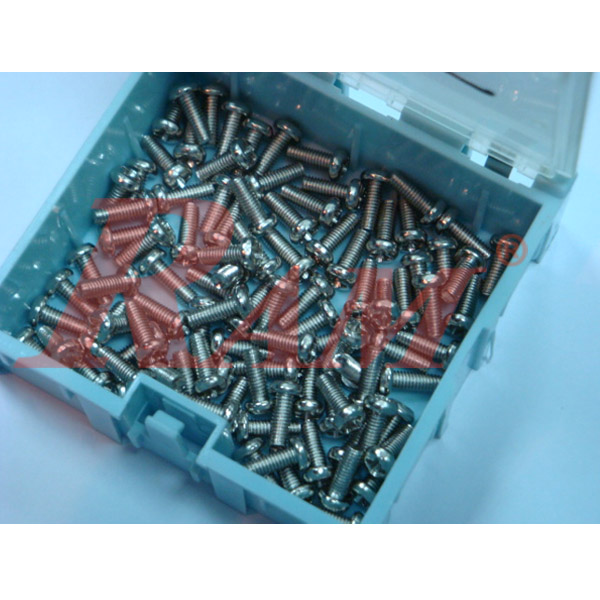
\includegraphics[width=0.9\linewidth, keepaspectratio]{images/components/bolts_m3.jpg} & M3 (various lengths) & Steel \\ \hline

\end{longtable}
\endgroup

\section{Detailed Mechanical Design}
\label{sec:detailed_mechanical_design}

\subsection{Chassis: Structure and Material}
\label{subsec:chassis_structure_material}
The main chassis forms the backbone of the robot, providing mounting points for all components and defining the robot's overall form factor.
The robot features a generally circular chassis, a common design choice for cleaning robots as it aids in maneuverability and helps the robot glance off obstacles rather than getting caught on corners, facilitating navigation in typical household environments.
The custom components were fabricated using \hyperref[term:pla]{PLA}+ filament via an \hyperref[term:fdm]{FDM} 3D printing service; PLA+ was the material offered by the service and is suitable for prototypes due to its ease of printing and adequate strength. Its rigidity is beneficial for creating a stable chassis that prevents flex, ensuring consistent alignment for the drive system and sensors. A substantial wall thickness of approximately 1 cm was utilized for the main structural components to ensure robustness and resistance to impacts during operation.
(Refer to Figure~\ref{fig:solidworks_chassis_views_combined} for detailed CAD views).

\begin{figure}[htbp]
    \centering
    \begin{subfigure}[b]{0.496\textwidth}
        \centering
        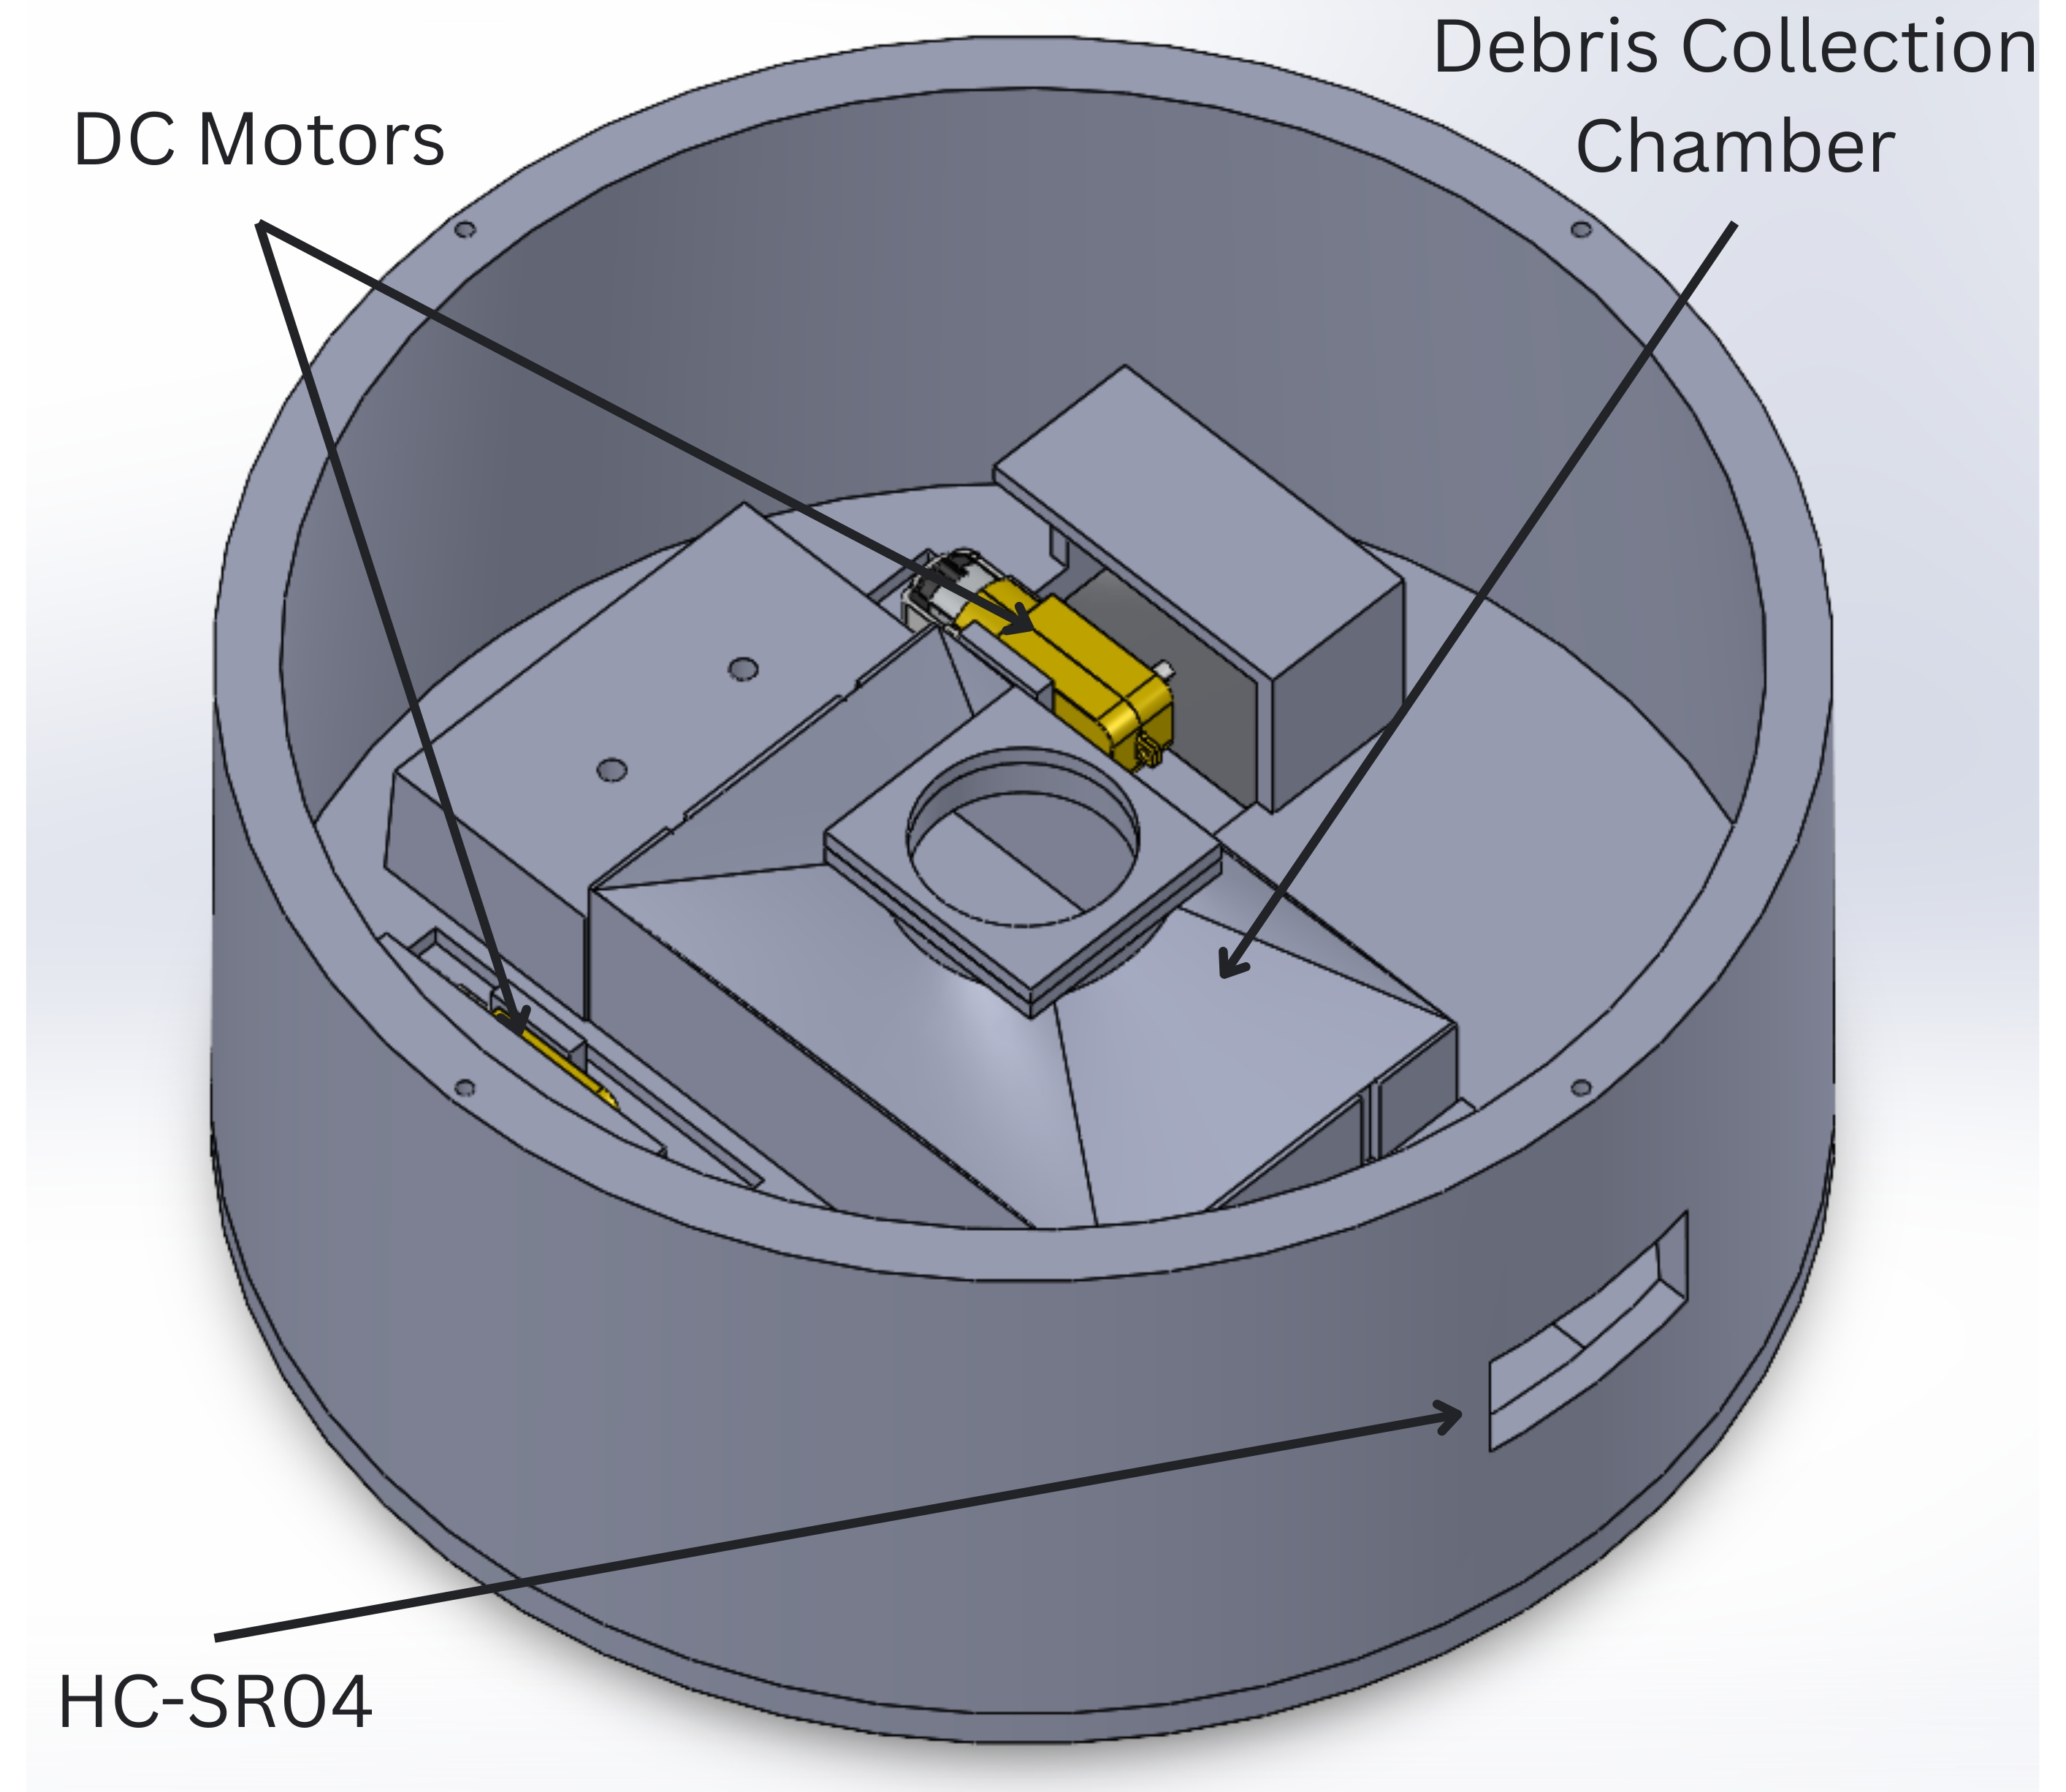
\includegraphics[width=\linewidth, keepaspectratio]{images/cad/chassis_open_isometric.jpg}
        \caption{Isometric view of the open chassis.}
        \label{fig:sw_chassis_iso_open}
    \end{subfigure}
    \hfill
    \begin{subfigure}[b]{0.496\textwidth}
        \centering
        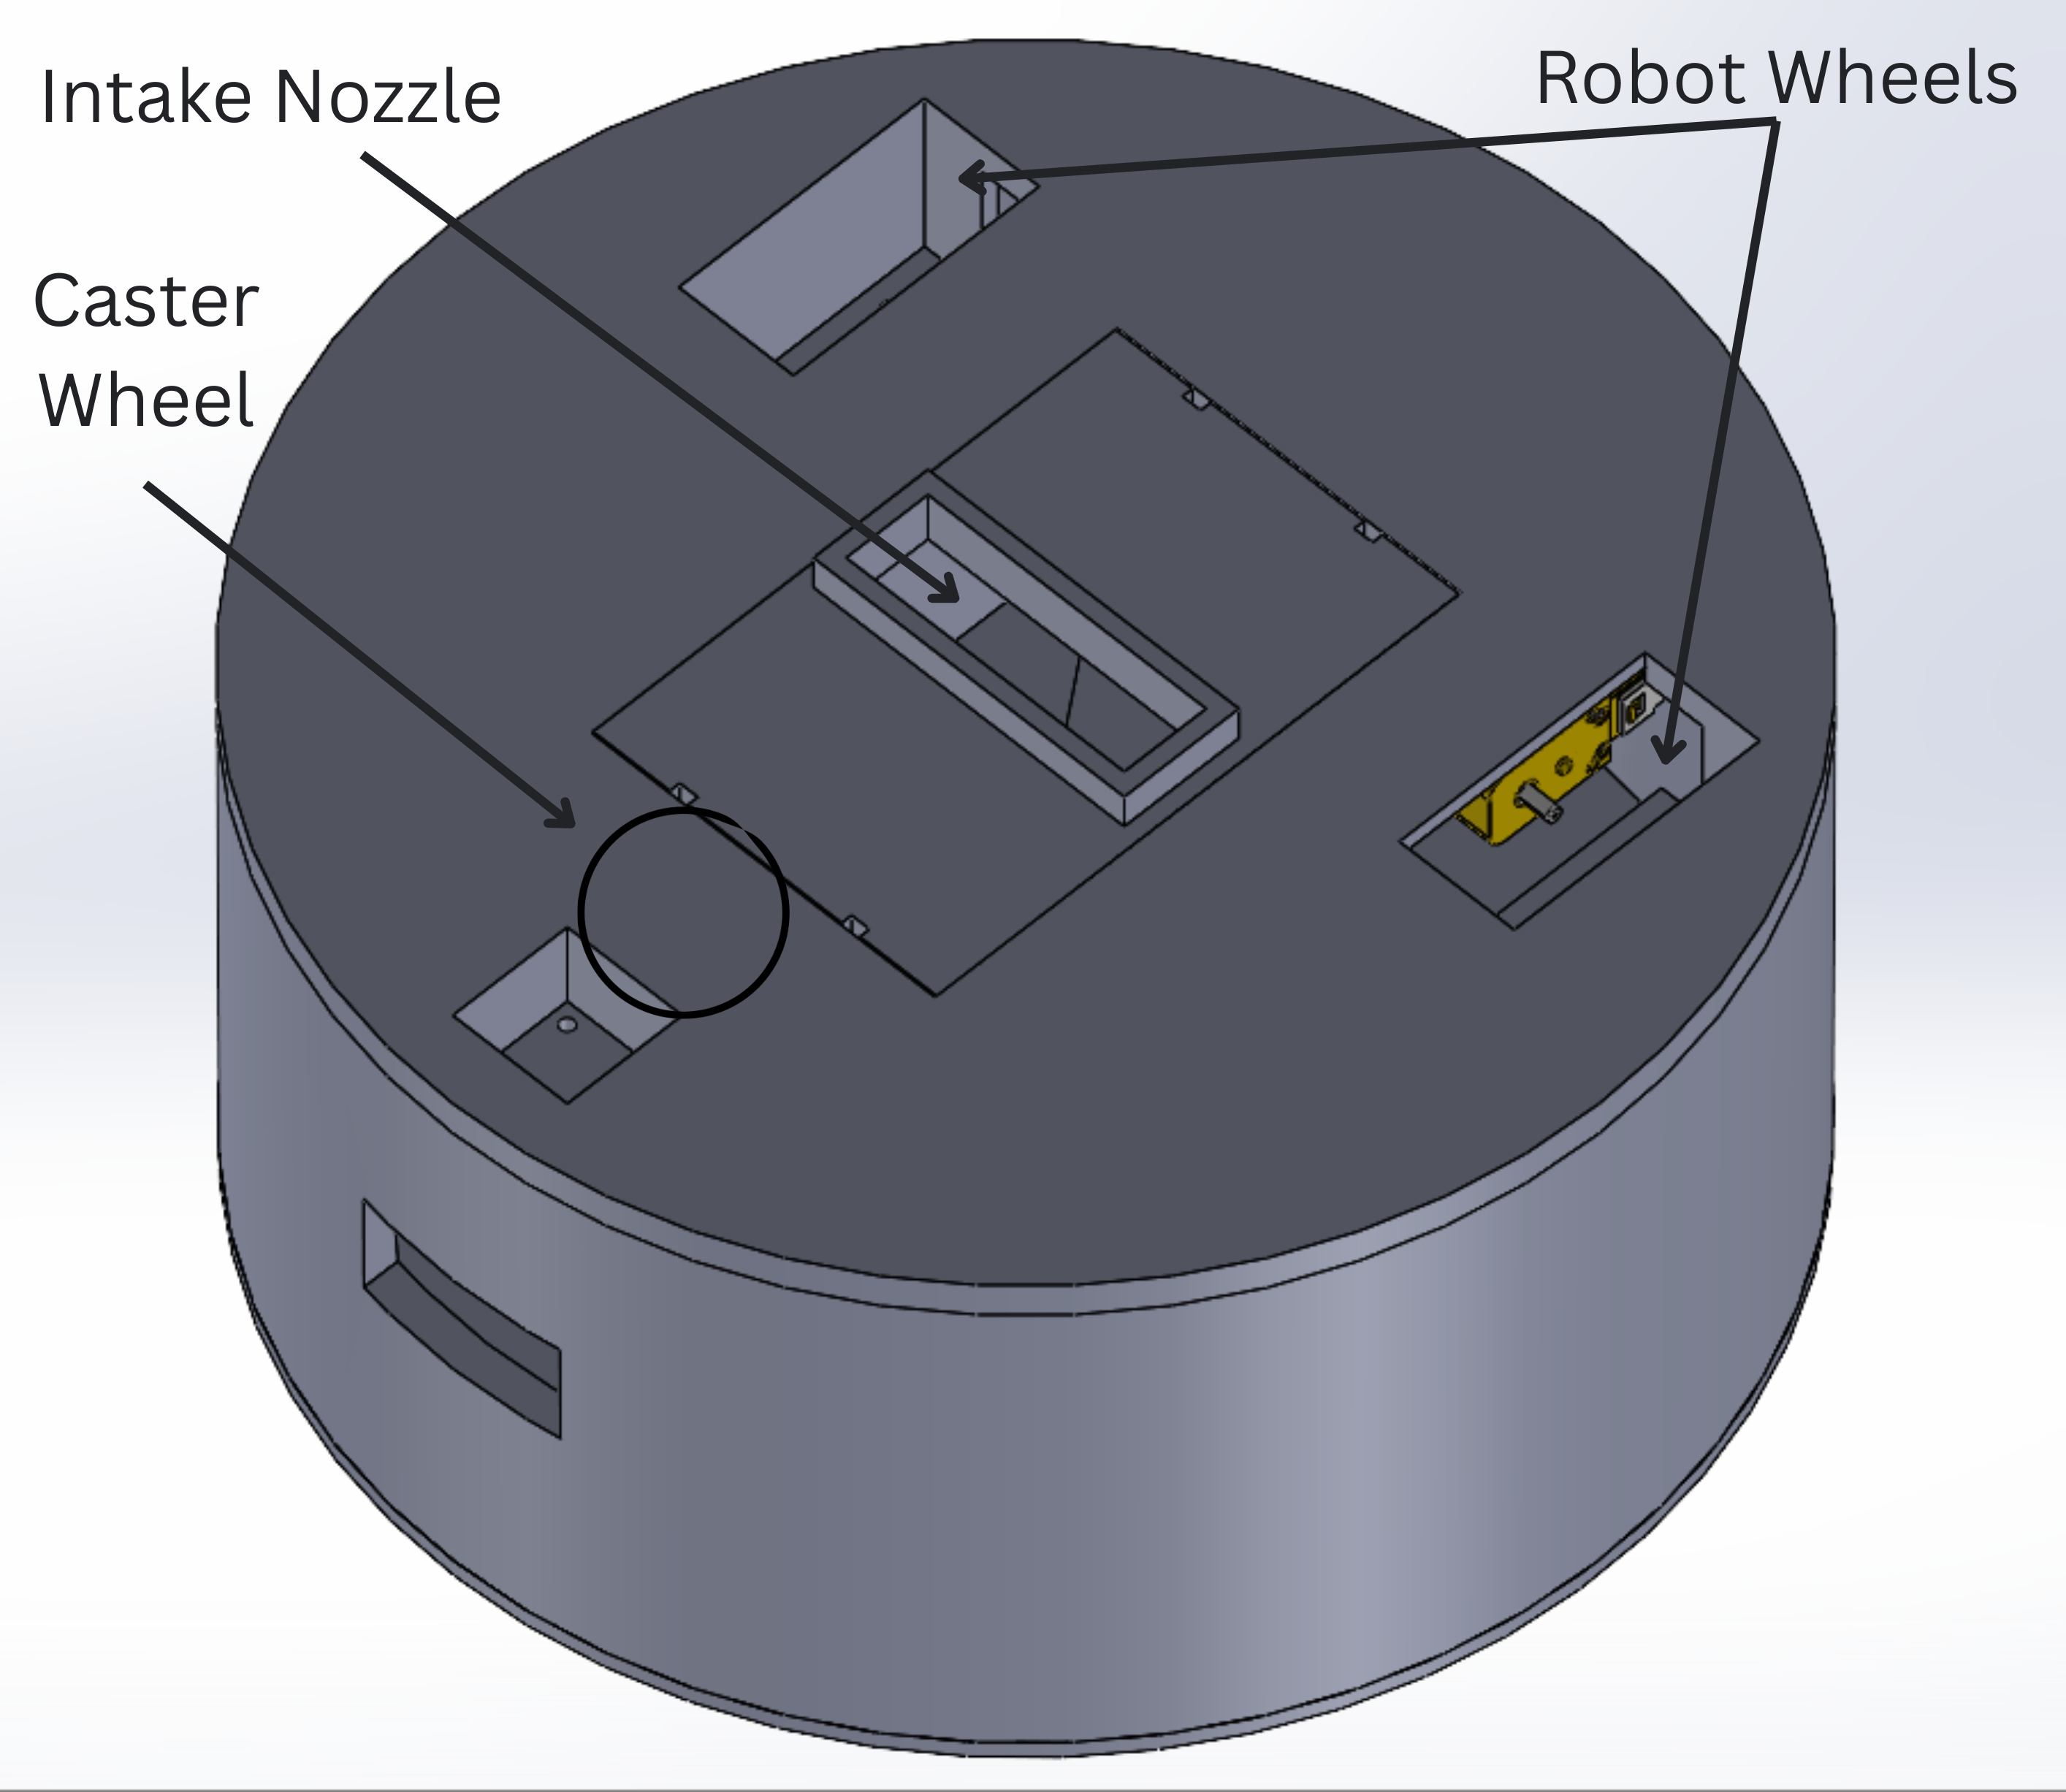
\includegraphics[width=\linewidth, keepaspectratio]{images/cad/chassis_bottom_view.jpg}
        \caption{Bottom CAD view of the chassis.}
        \label{fig:sw_chassis_bottom_cad}
    \end{subfigure}

    \vspace{10pt} % Adds a bit of vertical space between rows of subfigures

    \begin{subfigure}[b]{0.496\textwidth}
        \centering
        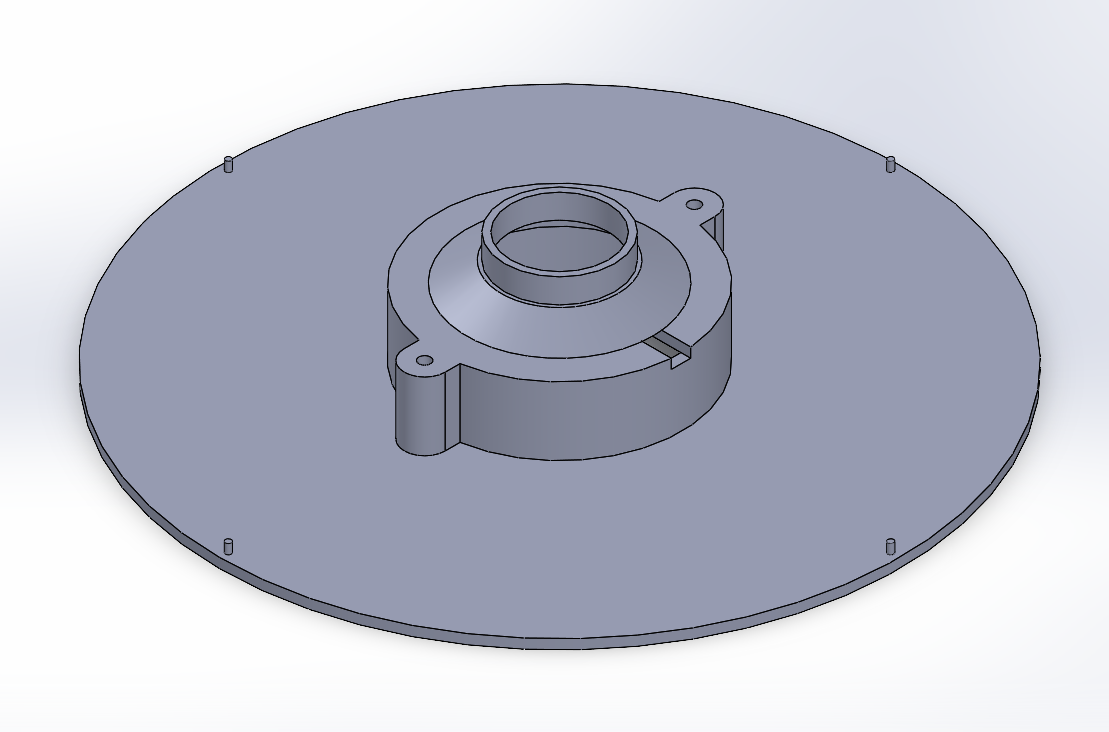
\includegraphics[width=\linewidth, keepaspectratio]{images/cad/chassis_lid_isometric.png}
        \caption{Isometric view of the main robot lid.}
        \label{fig:sw_chassis_lid_iso}
    \end{subfigure}
    \hfill
    \begin{subfigure}[b]{0.496\textwidth}
        \centering
        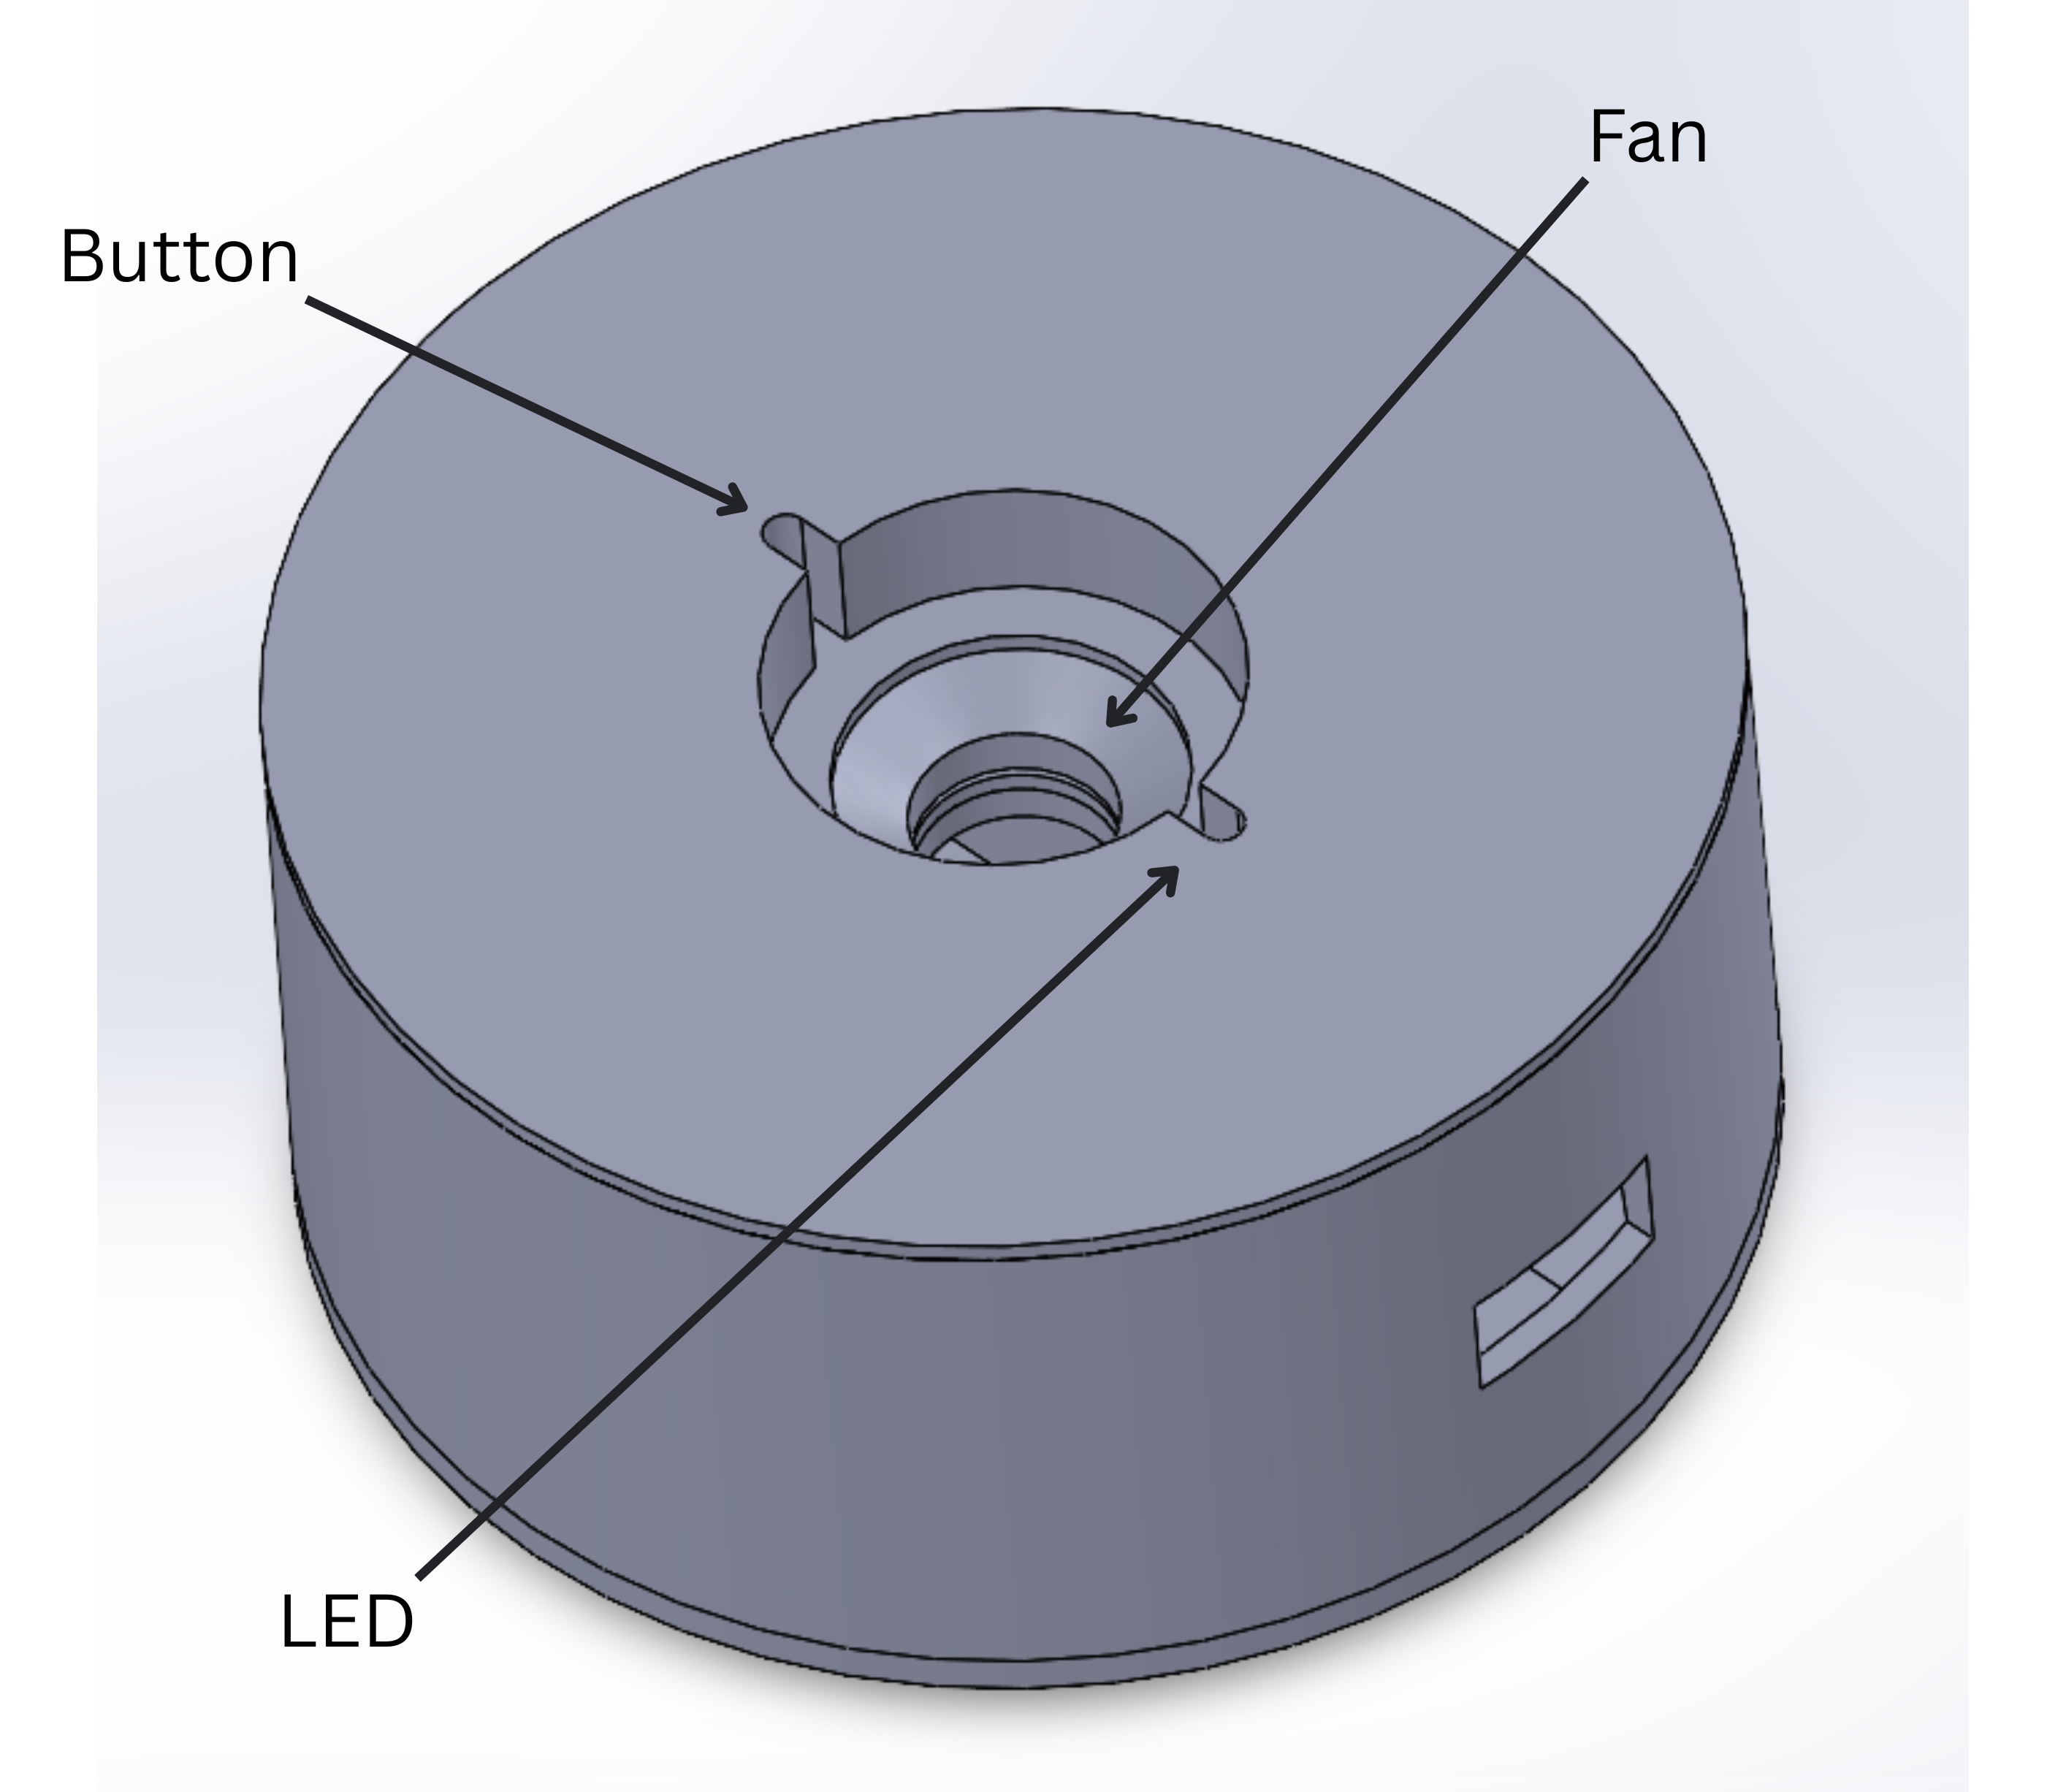
\includegraphics[width=\linewidth, keepaspectratio]{images/cad/chassis_assembled_isometric.jpg}
        \caption{Fully assembled robot isometric view.}
        \label{fig:sw_chassis_iso_closed}
    \end{subfigure}
    \caption{SolidWorks \hyperref[term:cad]{CAD} models illustrating the Smart Cleaning Robot's chassis and assembled form, with annotations to highlight key features.}
    \label{fig:solidworks_chassis_views_combined}
\end{figure}
The chassis is a custom design modeled in SolidWorks and 3D printed. It features:
\begin{itemize}
    \item \textbf{Base Plate}: Provides the primary mounting surface for motors, the caster wheel, and the Debris Collection Chamber. (See Figure~\ref{fig:sw_chassis_bottom_cad} and \ref{fig:sw_chassis_iso_open}). The 12V \hyperref[term:liion]{Li-ion} battery pack is secured between one of the debris chamber's guide blocks (discussed later) and a chassis wall, positioned towards the rear above the drive wheels to enhance traction.
    \item \textbf{Wheel Housings and Motor Mounting Points}: Located at the rear of the chassis, dedicated structures provide partial housing for the wheels. The two \hyperref[term:dc]{DC} gear motors are screwed into small, integrated walls on the chassis; these walls incorporate precise mounting holes and provide lateral support and alignment for the motors. (Visible in Figure~\ref{fig:sw_chassis_iso_open}). These structures were also designed to provide stable mounting points for the IR photoelectric sensors, ensuring the encoder discs that rotate with the wheels pass correctly through their sensing grooves.
    \item \textbf{Sensor Cutout and Mounting}: A dedicated cutout at the front of the chassis houses the \hyperref[term:hcsr04]{HC-SR04}  sensor. A custom bracket was designed to securely hold the sensor within this cutout, ensuring correct alignment for obstacle detection. (Visible in Figure~\ref{fig:sw_chassis_iso_open} and \ref{fig:sw_chassis_iso_closed}).
    \item \textbf{Front Caster Wheel Mount}: The front bottom section of the chassis includes a mounting point for the caster wheel. Due to the unavailability of the initially planned component, an alternative caster wheel was utilized, necessitating an adapted screw mounting method on the chassis base. (See Figure~\ref{fig:sw_chassis_bottom_cad} and Figure~\ref{fig:assembled_robot_bottom_photo}).
    \item \textbf{Central Cutout}: A large central cutout accommodates the Debris Collection Chamber. (Visible in Figure~\ref{fig:sw_chassis_bottom_cad}).
    \item \textbf{Electronics Mounting}: The custom \hyperref[term:pcb]{PCB} (which hosts the Raspberry Pi Pico W, LM2596S buck converter, and sensor voltage divider resistors) and the \hyperref[term:l298n]{L298N} H-bridge motor driver module are elevated from the chassis base using 20mm nylon snap-in rivet PCB spacers. This provides clearance for wiring and protection for the electronics.
\end{itemize}
\begin{figure}[htbp]
    \centering
    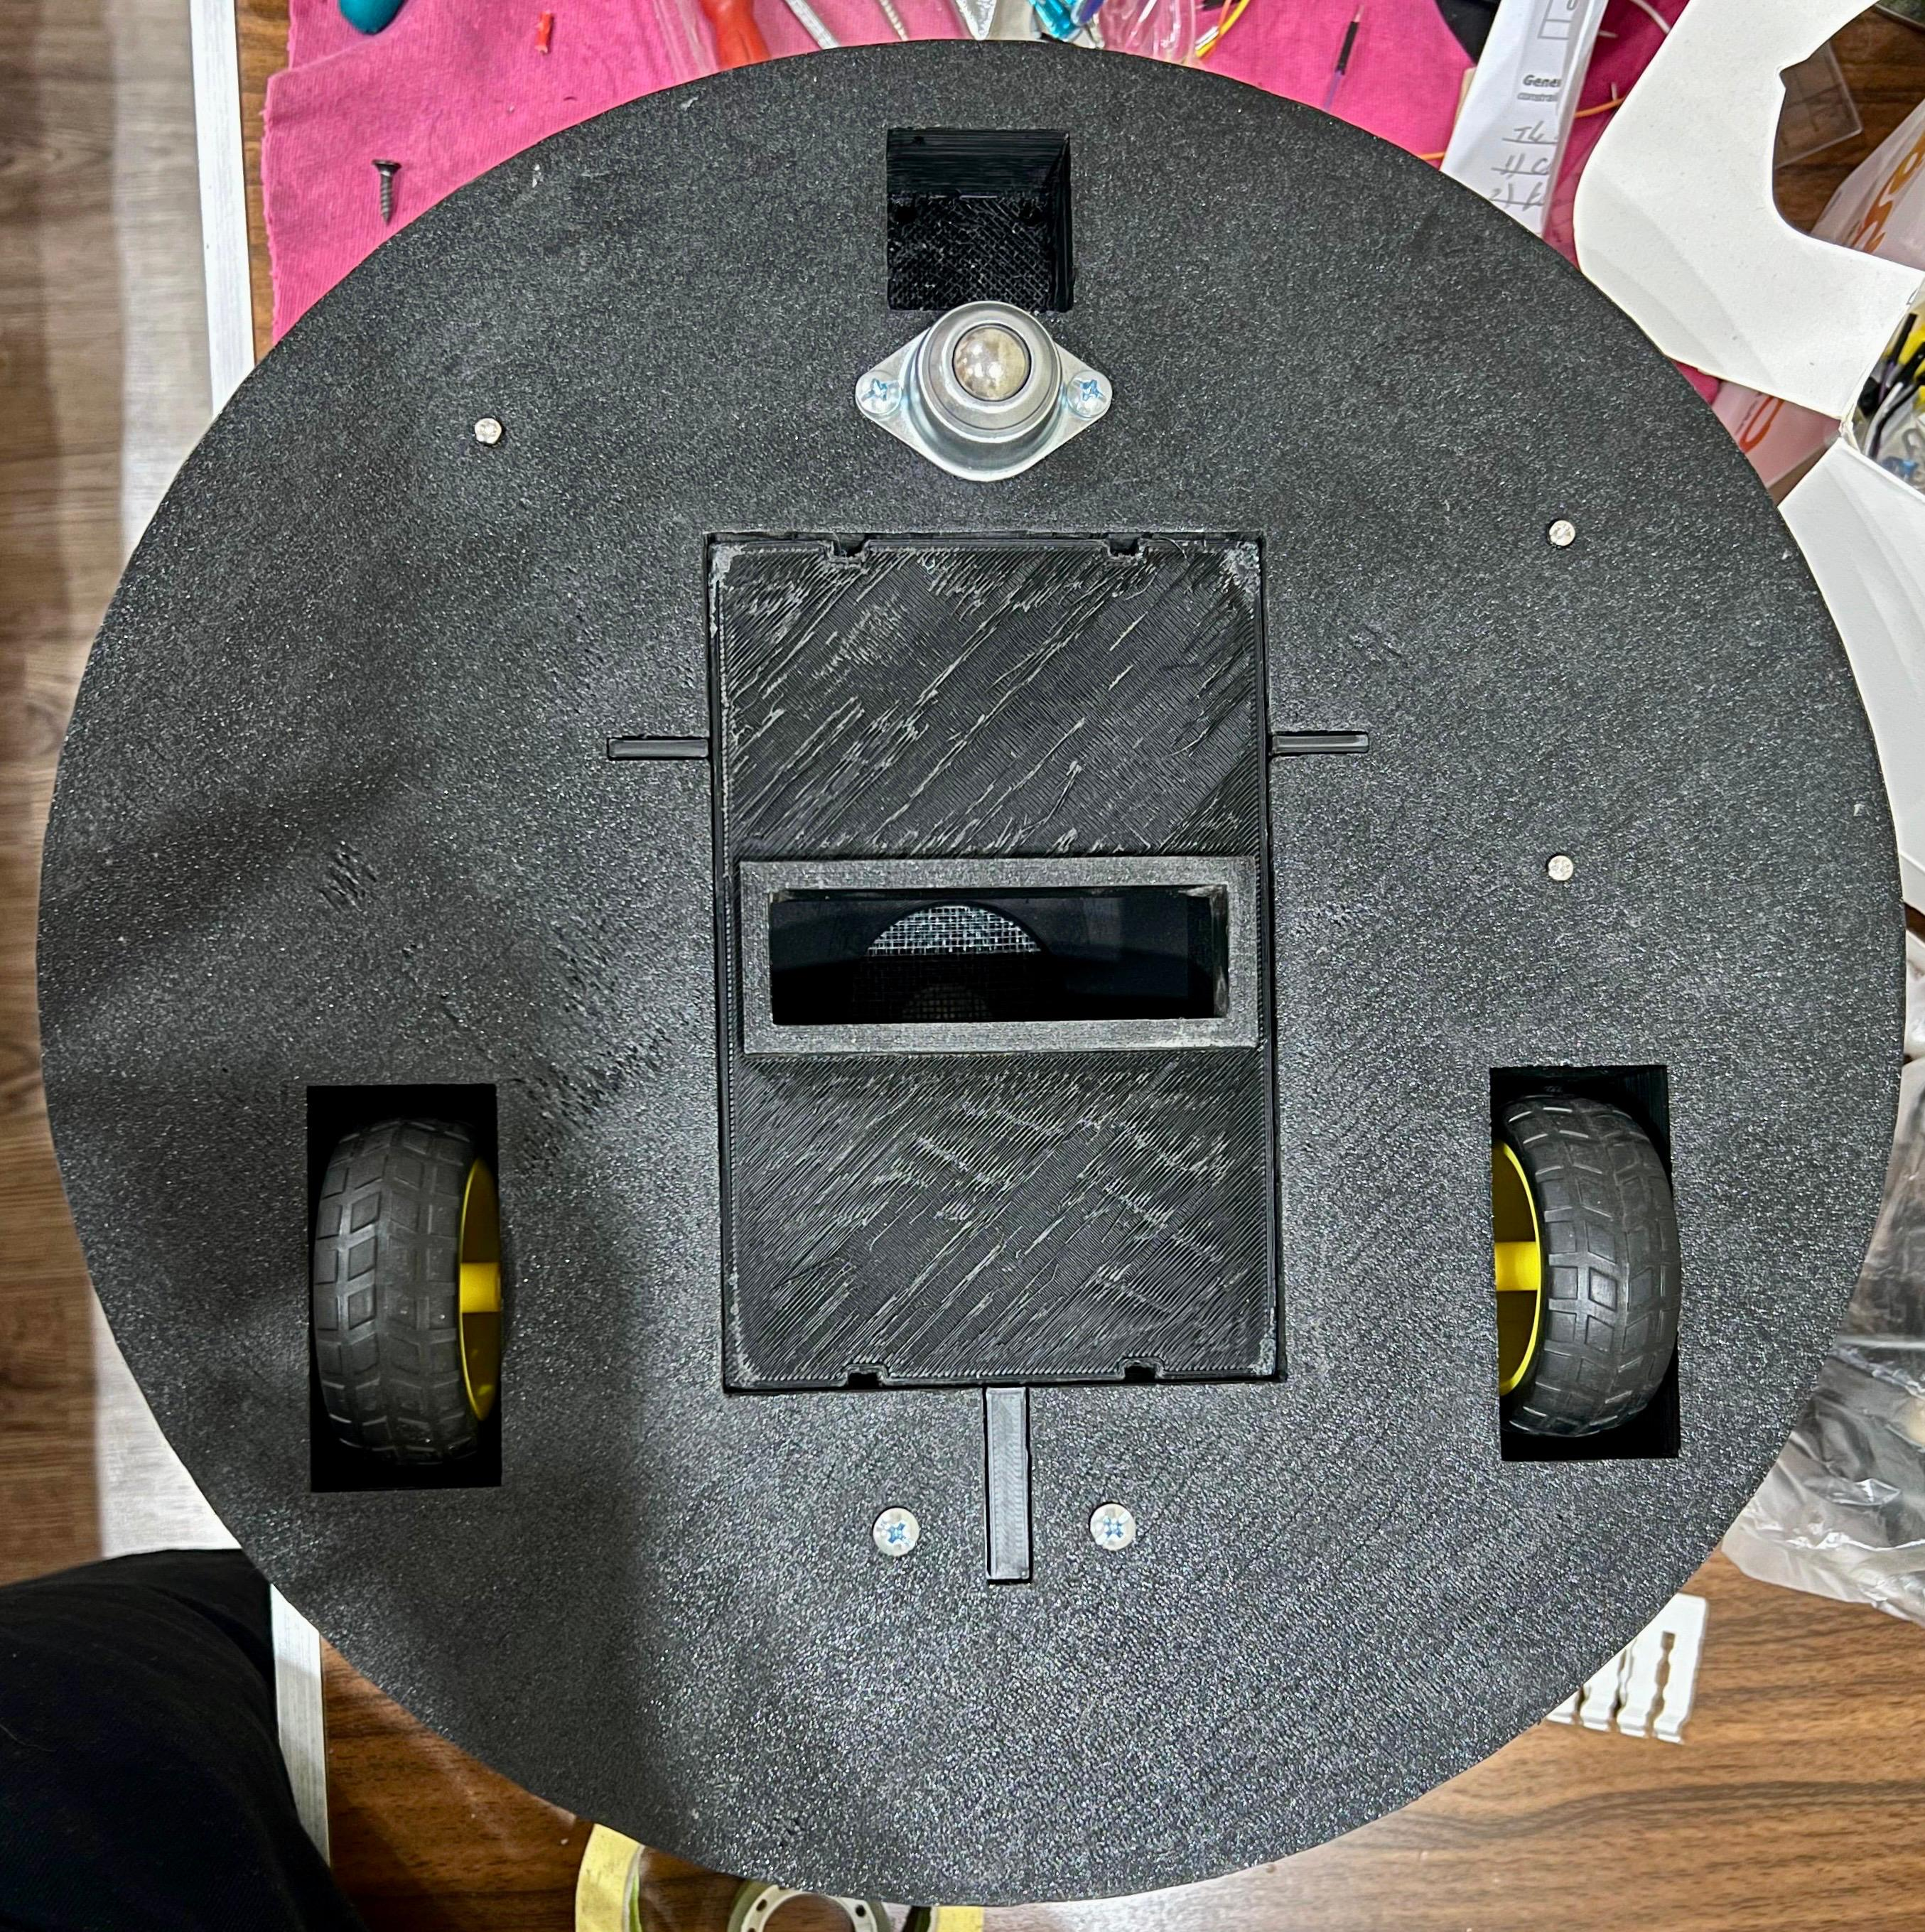
\includegraphics[width=0.75\textwidth, keepaspectratio]{images/photos/robot_bottom_photo.jpg}
    \caption{Bottom view photograph of the assembled Smart Cleaning Robot, showing the caster wheel, drive wheels, and vacuum intake nozzle.}
    \label{fig:assembled_robot_bottom_photo}
\end{figure}


\subsection{Vacuum System Design}
\label{subsec:vacuum_system_design_detailed}
The Debris Collection Chamber is a key sub-assembly designed to collect vacuumed particles. The chamber was designed for a tight clearance fit within the chassis bay to ensure stability and prevent rattling. (See Figure~\ref{fig:solidworks_debris_chamber} for its CAD design and Figure~\ref{fig:debris_chamber_photo} for a photo of the 3D printed part).
\begin{itemize}
    \item \textbf{Chamber Design}: The chamber itself is a custom 3D-printed component. It features a rectangular box base measuring 10.5\,cm in width, 16\,cm in length, and 5.5\,cm in height. From this base, the chamber transitions through a pyramid-like section for an additional 2.5\,cm in height, culminating in a circular outlet of 5\,cm in diameter. This outlet is designed to interface with the vacuum fan and also seats the air filter. The debris inlet, located at the bottom of the chamber, has dimensions of 8.5\,cm x 2.5\,cm.
    \item \textbf{Mounting and Guides}: The method for positioning the chamber within the chassis was refined during development (detailed in Section~\ref{sec:mechanical_assembly_implementation_new}). The final design uses two robust 3D-printed blocks screwed to the chassis base, incorporating guide elements for secure and precise placement.
    \item \textbf{Filter and Lid}: A removable lid is designed for the top of the Debris Collection Chamber to hold an air filter. This lid fits into corresponding features on the chamber for easy removal and a secure fit. The main robot chassis lid (Figure~\ref{fig:sw_chassis_lid_iso}), when closed, presses down on this filter lid, keeping it secure.
\end{itemize}

\begin{figure}[htbp]
    \centering
    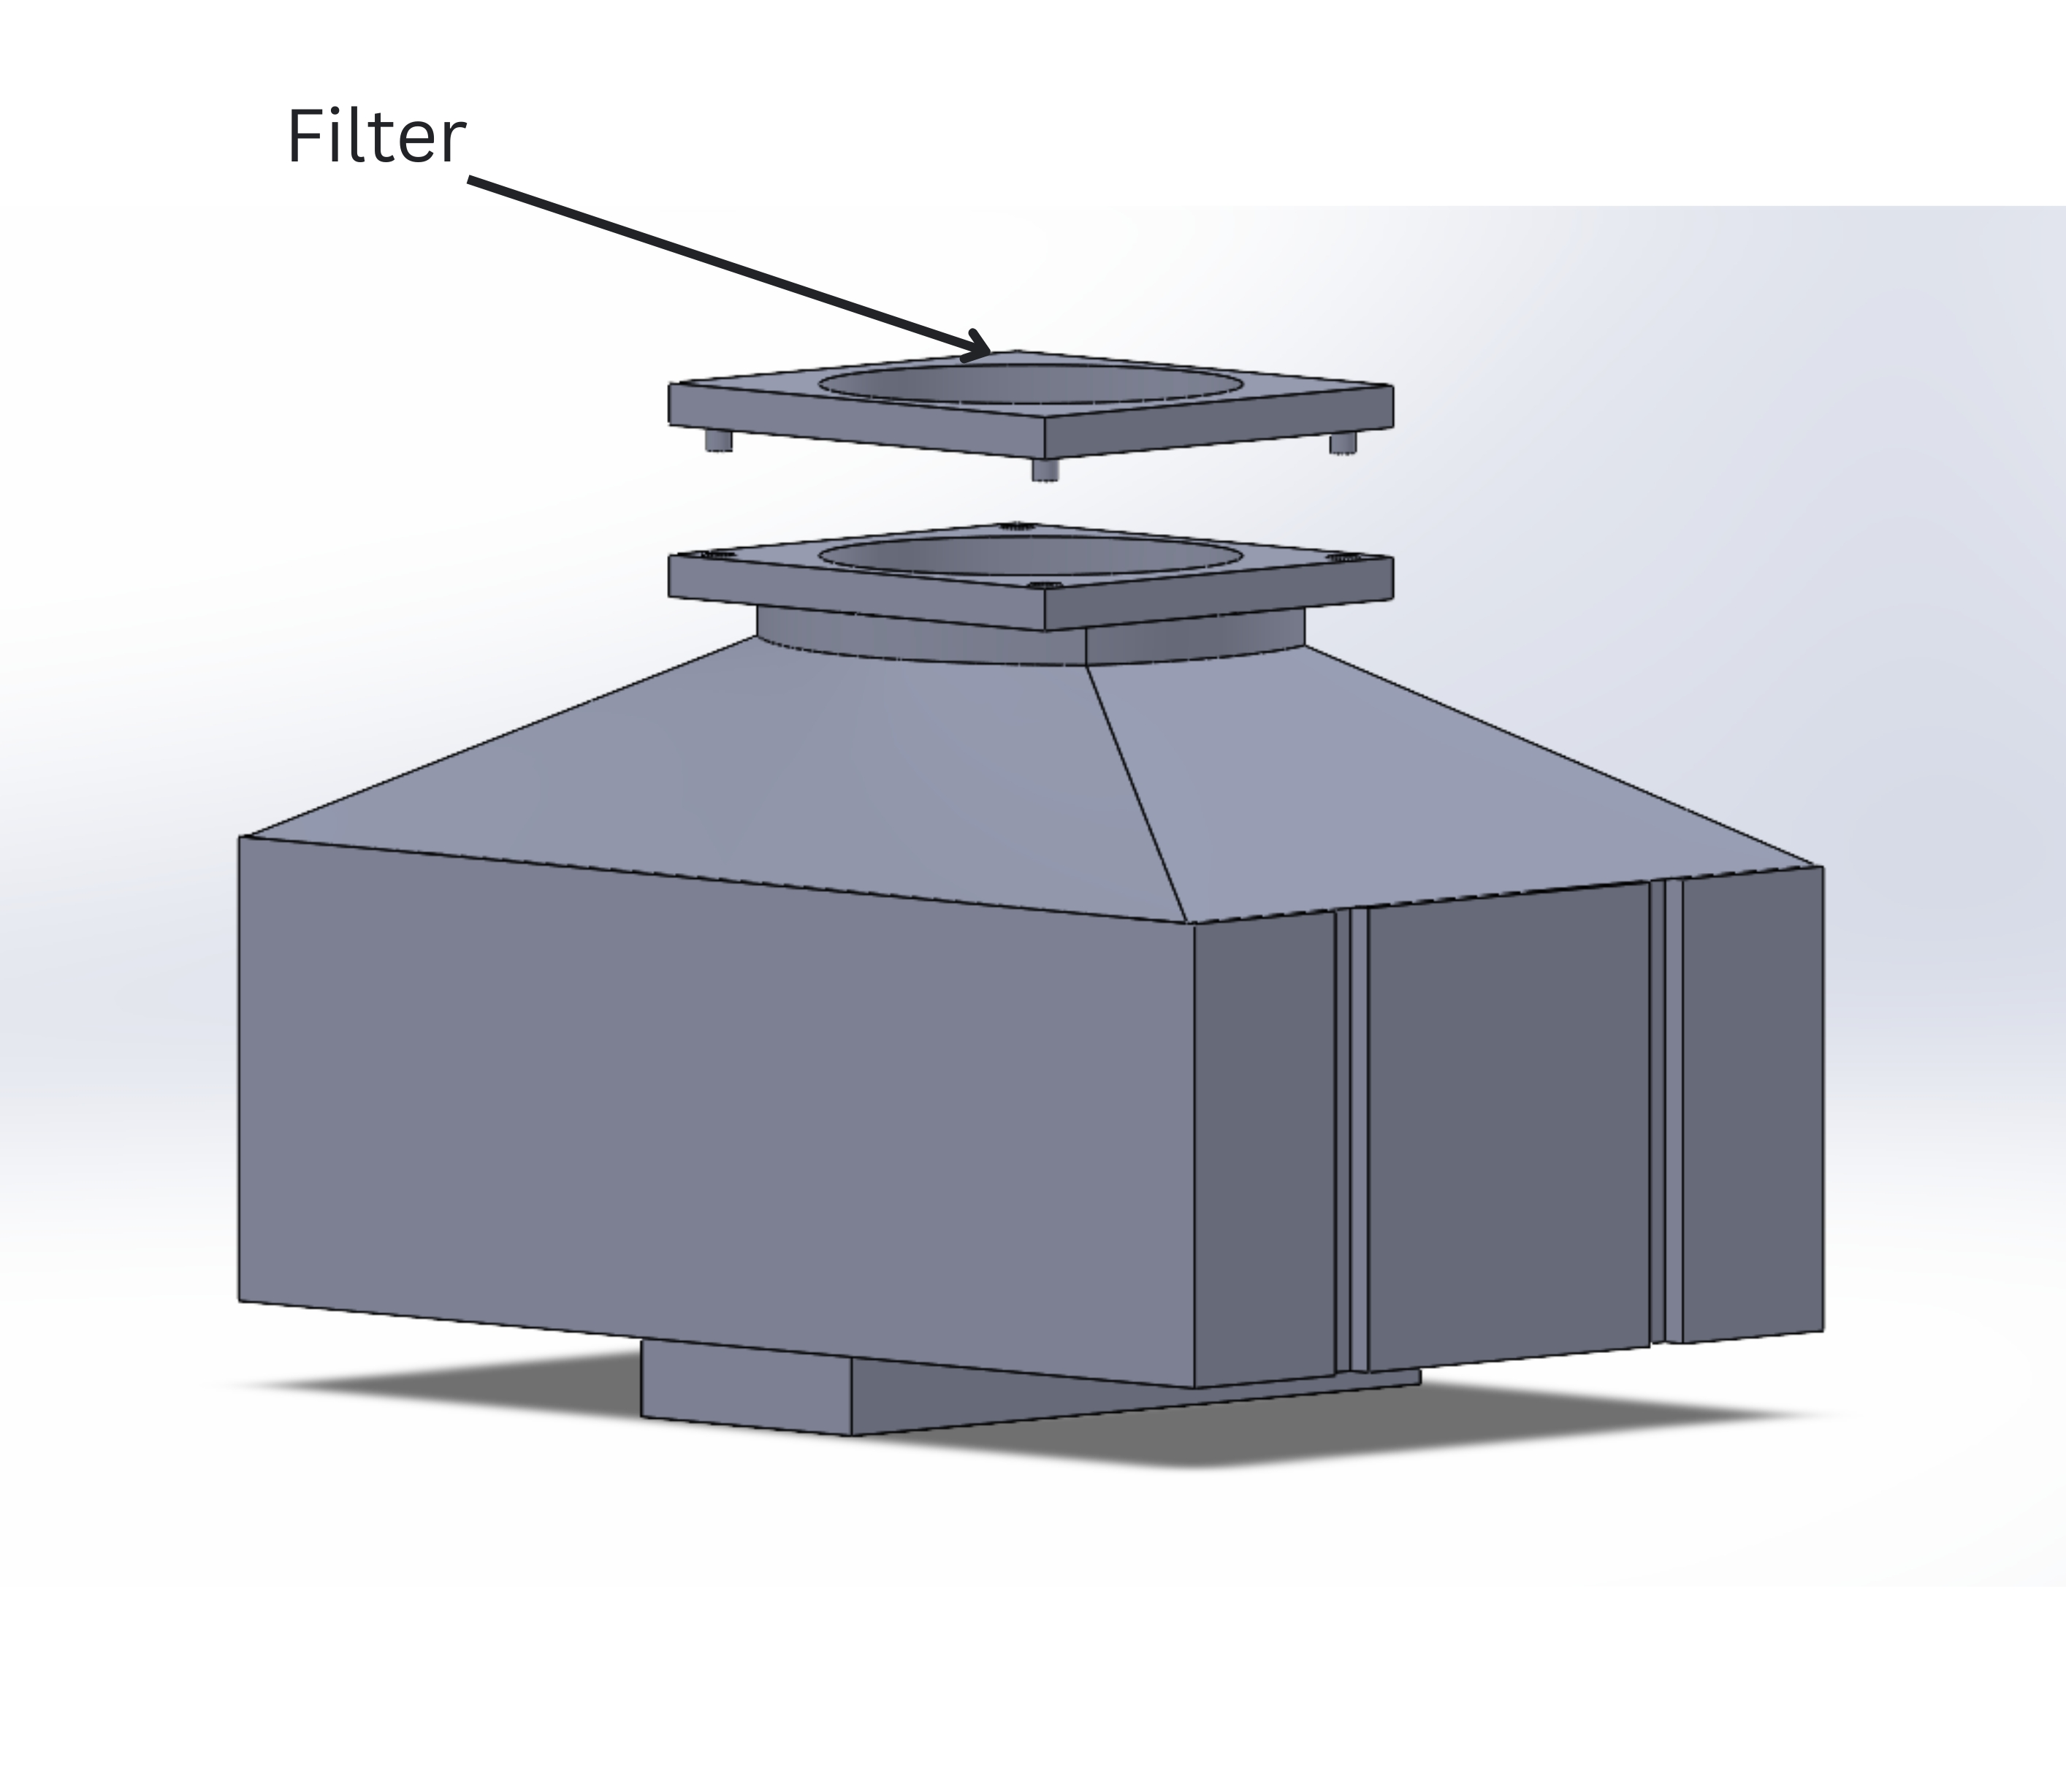
\includegraphics[width=1\textwidth, keepaspectratio]{images/cad/debris_chamber_cad.jpg}
    \caption{SolidWorks CAD design of the Debris Collection Chamber.}
    \label{fig:solidworks_debris_chamber}
\end{figure}
\begin{figure}[htbp]
    \centering
    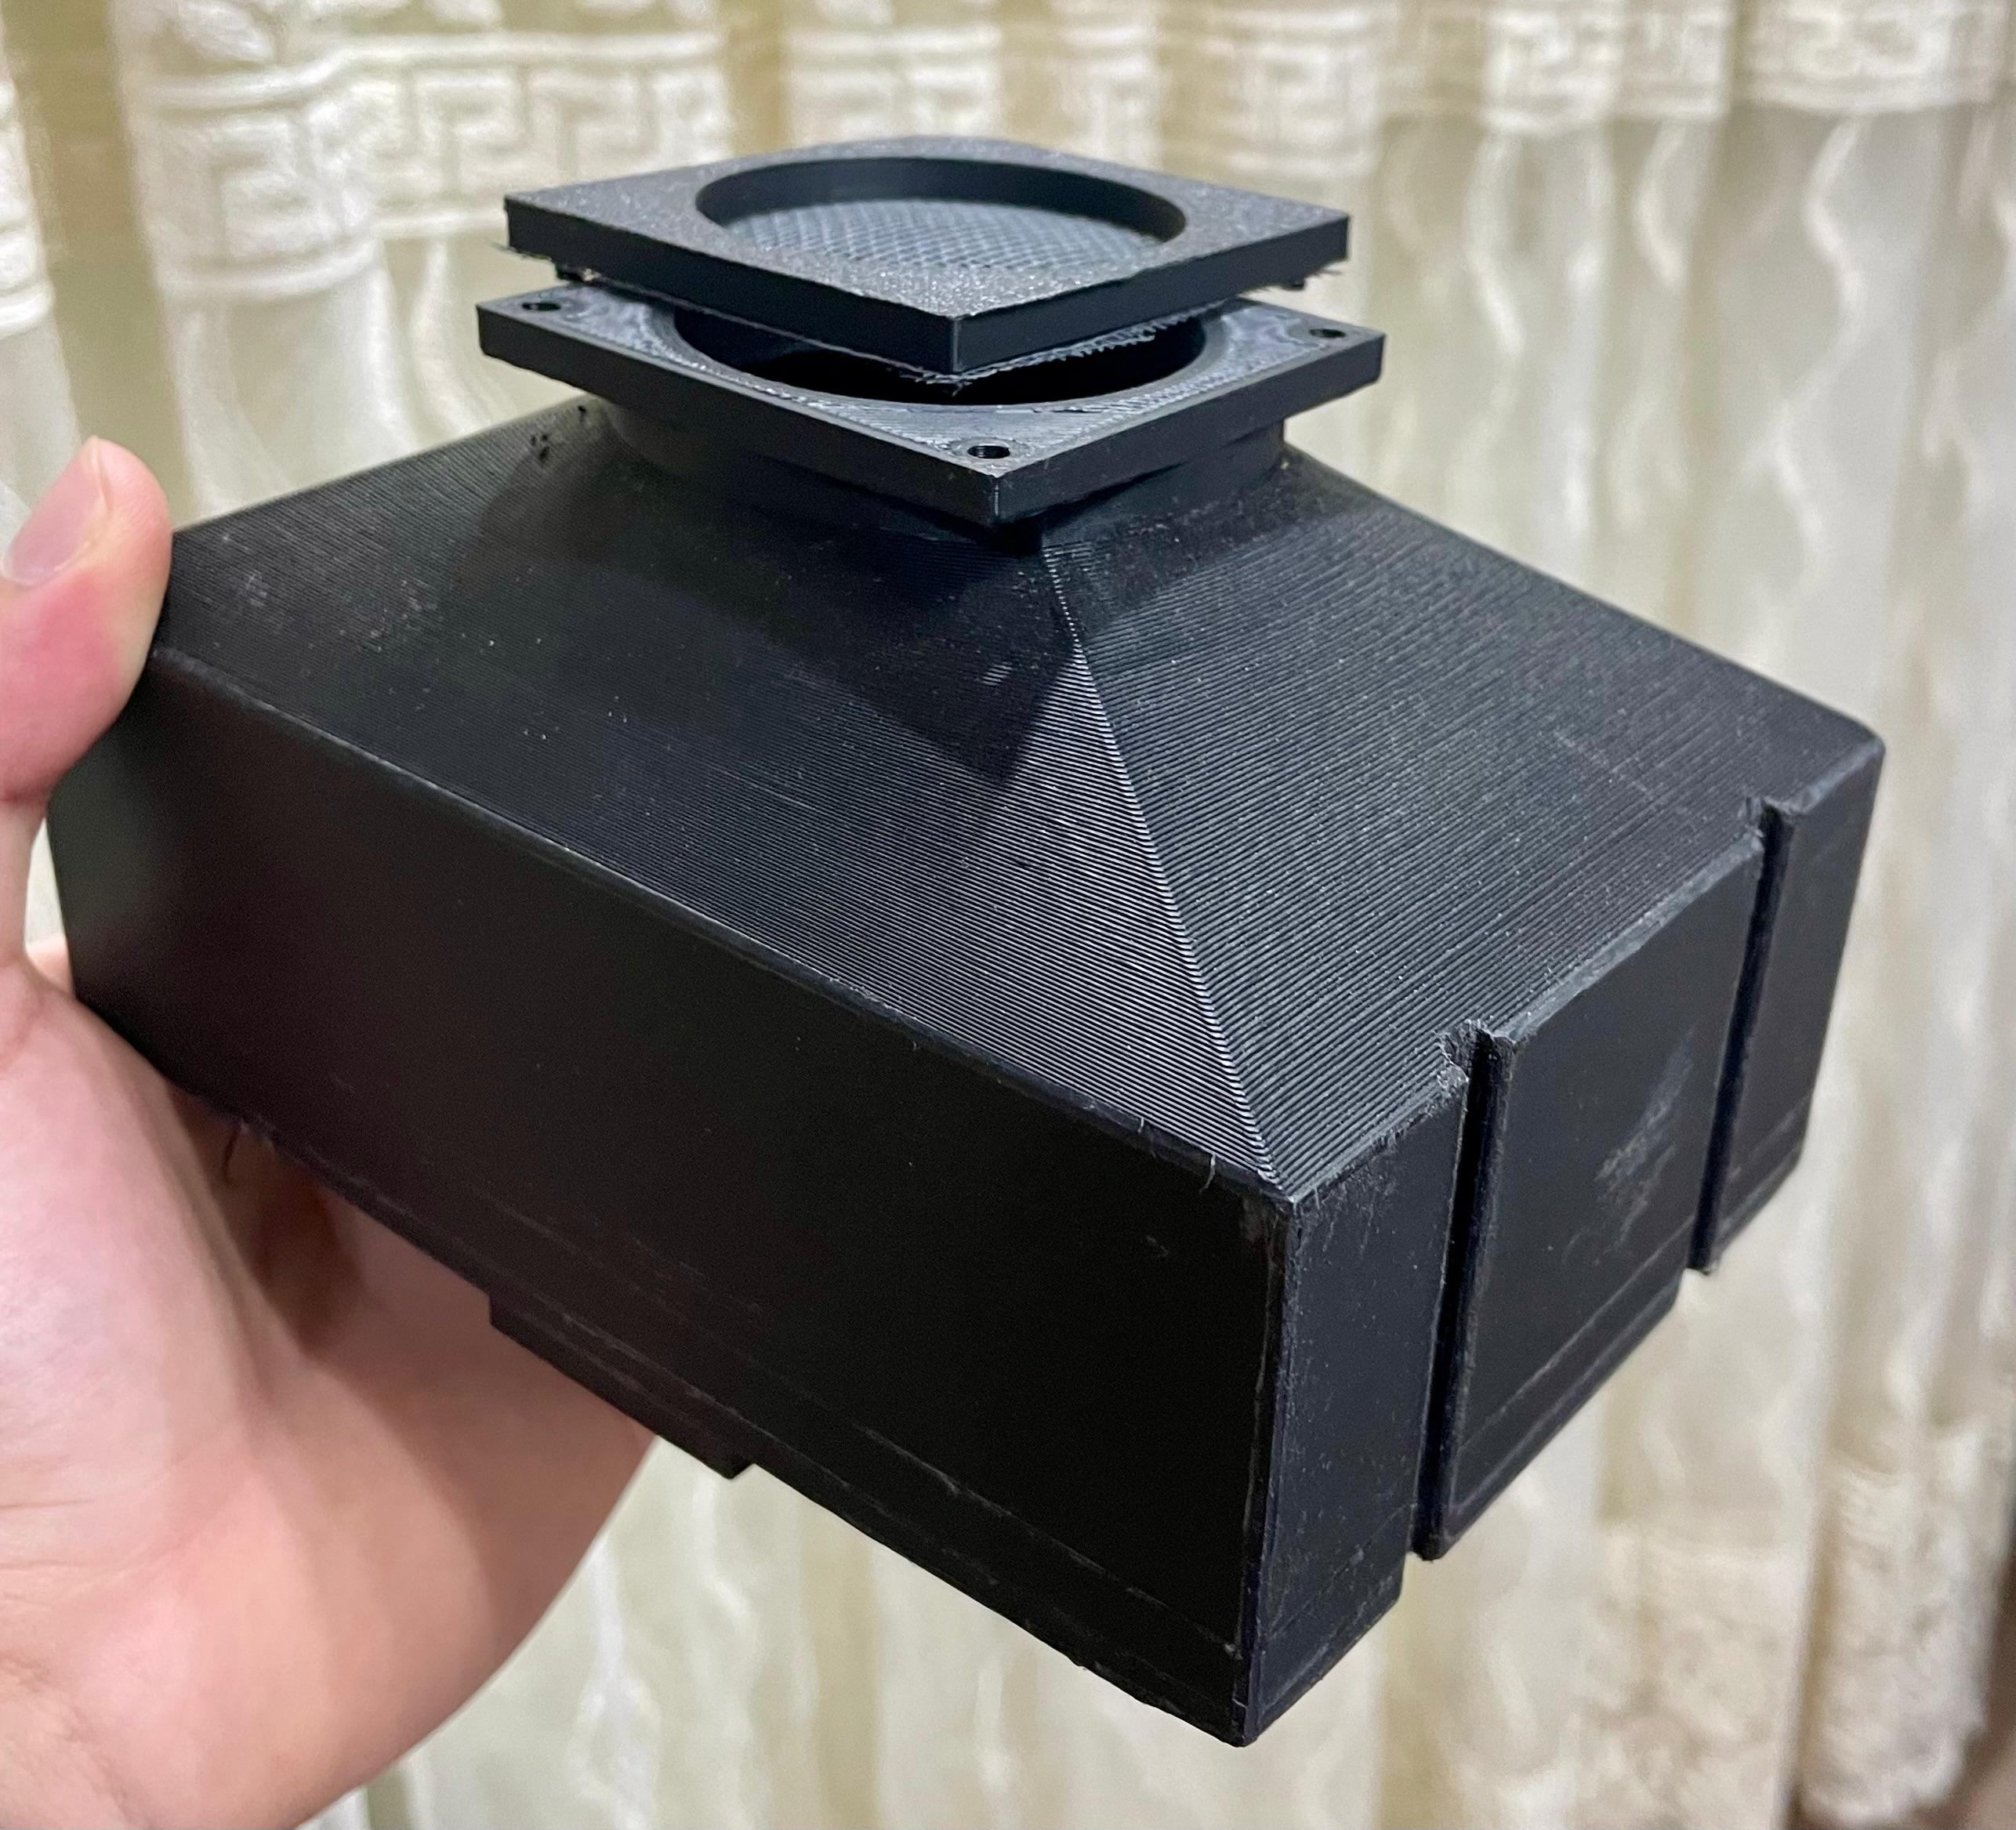
\includegraphics[width=0.75\textwidth, keepaspectratio]{images/photos/debris_chamber_photo.jpg}
    \caption{Photograph of the 3D printed Debris Collection Chamber with its removable filter lid.}
    \label{fig:debris_chamber_photo}
\end{figure}

The vacuum system is responsible for generating airflow to collect debris.
\begin{itemize}
    \item \textbf{Fan Selection and Mounting}: The primary vacuum source is a repurposed PS3 fan (Model: Delta KSB1012HE)~\cite{DeltaKSB1012HE_PSDevWiki}. This fan was readily available and met basic size and 12V \hyperref[term:dc]{DC} voltage requirements. It has a diameter of approximately 10cm and features 17 blades.
    The fan is mounted within the main top lid of the robot (see Figure~\ref{fig:sw_chassis_lid_iso}).
    \item \textbf{Airflow Path}: Air is drawn through an intake nozzle (part of the Debris Collection Chamber design, Figure~\ref{fig:solidworks_debris_chamber}), passes through the filter in the chamber's lid, then through the fan, and is exhausted from the robot. The debris chamber was designed to channel airflow with minimal obstruction.
\end{itemize}

\subsection{Drive System Design}
\label{subsec:drive_system_design_detailed}
The drive system enables the robot's mobility. A differential drive configuration was selected for its simplicity in control, maneuverability (allowing for zero-radius turns), and common availability of components.
\begin{itemize}
    \item \textbf{Motors and Wheels}: Two \hyperref[term:dc]{DC} gear motors (TT type) provide locomotion, each driving a 66mm diameter wheel. These are mounted in dedicated compartments at the rear of the chassis. (Visible in Figure~\ref{fig:sw_chassis_iso_open} and \ref{fig:sw_chassis_bottom_cad}).
    \item \textbf{Encoder Integration}: To enable precise movement control, a 20-slot plastic encoder disc was press-fit onto the interior side of each wheel's axle. An IR photoelectric sensor was mounted on the chassis such that the encoder disc passes through its 5mm groove. This setup allows for the measurement of wheel rotation, as detailed in Figure~\ref{fig:encoder_mechanism}.
    \item \textbf{Caster Wheel}: A caster wheel at the front provides a third point of contact, allowing for maneuverability and stable turns. As noted, the mounting of this wheel was adapted due to component availability. (Visible in Figure~\ref{fig:sw_chassis_bottom_cad} and Figure~\ref{fig:assembled_robot_bottom_photo}).
\end{itemize}

\begin{figure}[htbp]
    \centering
    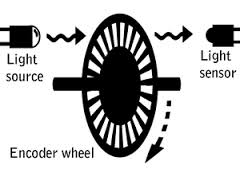
\includegraphics[width=0.47\textwidth]{images/components/encoder_disc_mounted.jpg}
    \caption{Diagram illustrating the principle of operation for the optical wheel encoder. As the encoder wheel (slotted disc) rotates with the main robot wheel, its slots alternately block and pass the light beam from the source to the sensor, generating a digital pulse train that corresponds to the distance traveled.}
    \label{fig:encoder_mechanism}
\end{figure}

\subsection{Main Robot Lid and Component Fastening}
\label{subsec:main_robot_lid_fastening_detailed}
The top lid of the robot (Figure~\ref{fig:sw_chassis_lid_iso}) serves multiple functions: it encloses the internal components, supports the vacuum fan assembly, presses down to secure the filter lid of the Debris Collection Chamber, and provides mounting points for an \hyperref[term:led]{LED} indicator and a power button. The main top lid incorporates dedicated openings for the power button and \hyperref[term:led]{LED} indicator, positioned conveniently next to the fan exhaust; these components are secured via friction fit. The method for securing the main top lid to the chassis was refined from an initial concept of small 3D-printed latching pieces to a more robust solution using four screws (detailed in Section~\ref{sec:mechanical_assembly_implementation_new}). The accessibility of the battery for charging was considered in the overall assembly.
\section{Mechanical Assembly Implementation}
\label{sec:mechanical_assembly_implementation_new}
The implementation process for the mechanical structure involved the fabrication of custom parts using an \hyperref[term:fdm]{FDM} 3D printer with \hyperref[term:pla]{PLA}+ filament (provided by a 3D printing service), and the assembly of all mechanical components onto the chassis.

The mechanical assembly followed a structured sequence:
\begin{enumerate}
    \item The two \hyperref[term:dc]{DC} gear motors and the front caster wheel were first secured to the 3D-printed chassis base.
    \item The custom 3D-printed Debris Collection Chamber was then slotted into its designated bay within the chassis.
    \item Electronic components, including the custom \hyperref[term:pcb]{PCB} (hosting the Raspberry Pi Pico W, LM2596S buck converter, and associated circuitry) and the \hyperref[term:l298n]{L298N} motor driver, were mounted onto their respective PCB spacers, which were affixed to the chassis. (The internal arrangement and wiring are detailed in Chapter~\ref{chap:electrical_control_performance}, Figure~\ref{fig:internal_wiring_photo_eval_new}).
    \item Essential wiring connections between the motors, sensors, \hyperref[term:pcb]{PCB}, and power components were then routed and made.
    \item The PS3 fan was installed into its housing within the main top lid.
    \item Finally, the top lid, with the fan, power button, and \hyperref[term:led]{LED} indicator secured, was fastened to the main chassis using four M3 screws, enclosing the internal components.
\end{enumerate}
An iterative design approach was crucial for refining certain mechanical aspects. For instance, the initial design for positioning the Debris Collection Chamber using slender guides proved too fragile. This was rectified by redesigning the mounting system to use two larger, screwed-in blocks with improved guide elements for precise placement and durability. Similarly, the main top lid fastening was changed from small latching pieces, found to be insufficiently robust against fan vibrations, to a more secure four-screw system. Minor adjustments, such as reaming mounting holes, were made as needed during assembly to ensure proper alignment and securement, a common practice in prototyping.

Figure~\ref{fig:assembled_robot_photos_eval_new} shows photographs of the fully 3D printed and assembled robot prototype. (The internal view showing component wiring and \hyperref[term:pcb]{PCB} integration is presented in Chapter~\ref{chap:electrical_control_performance}, Figure~\ref{fig:internal_wiring_photo_eval_new}).

\begin{figure}[htbp]
    \centering
    \begin{subfigure}[b]{0.496\textwidth}
        \centering
        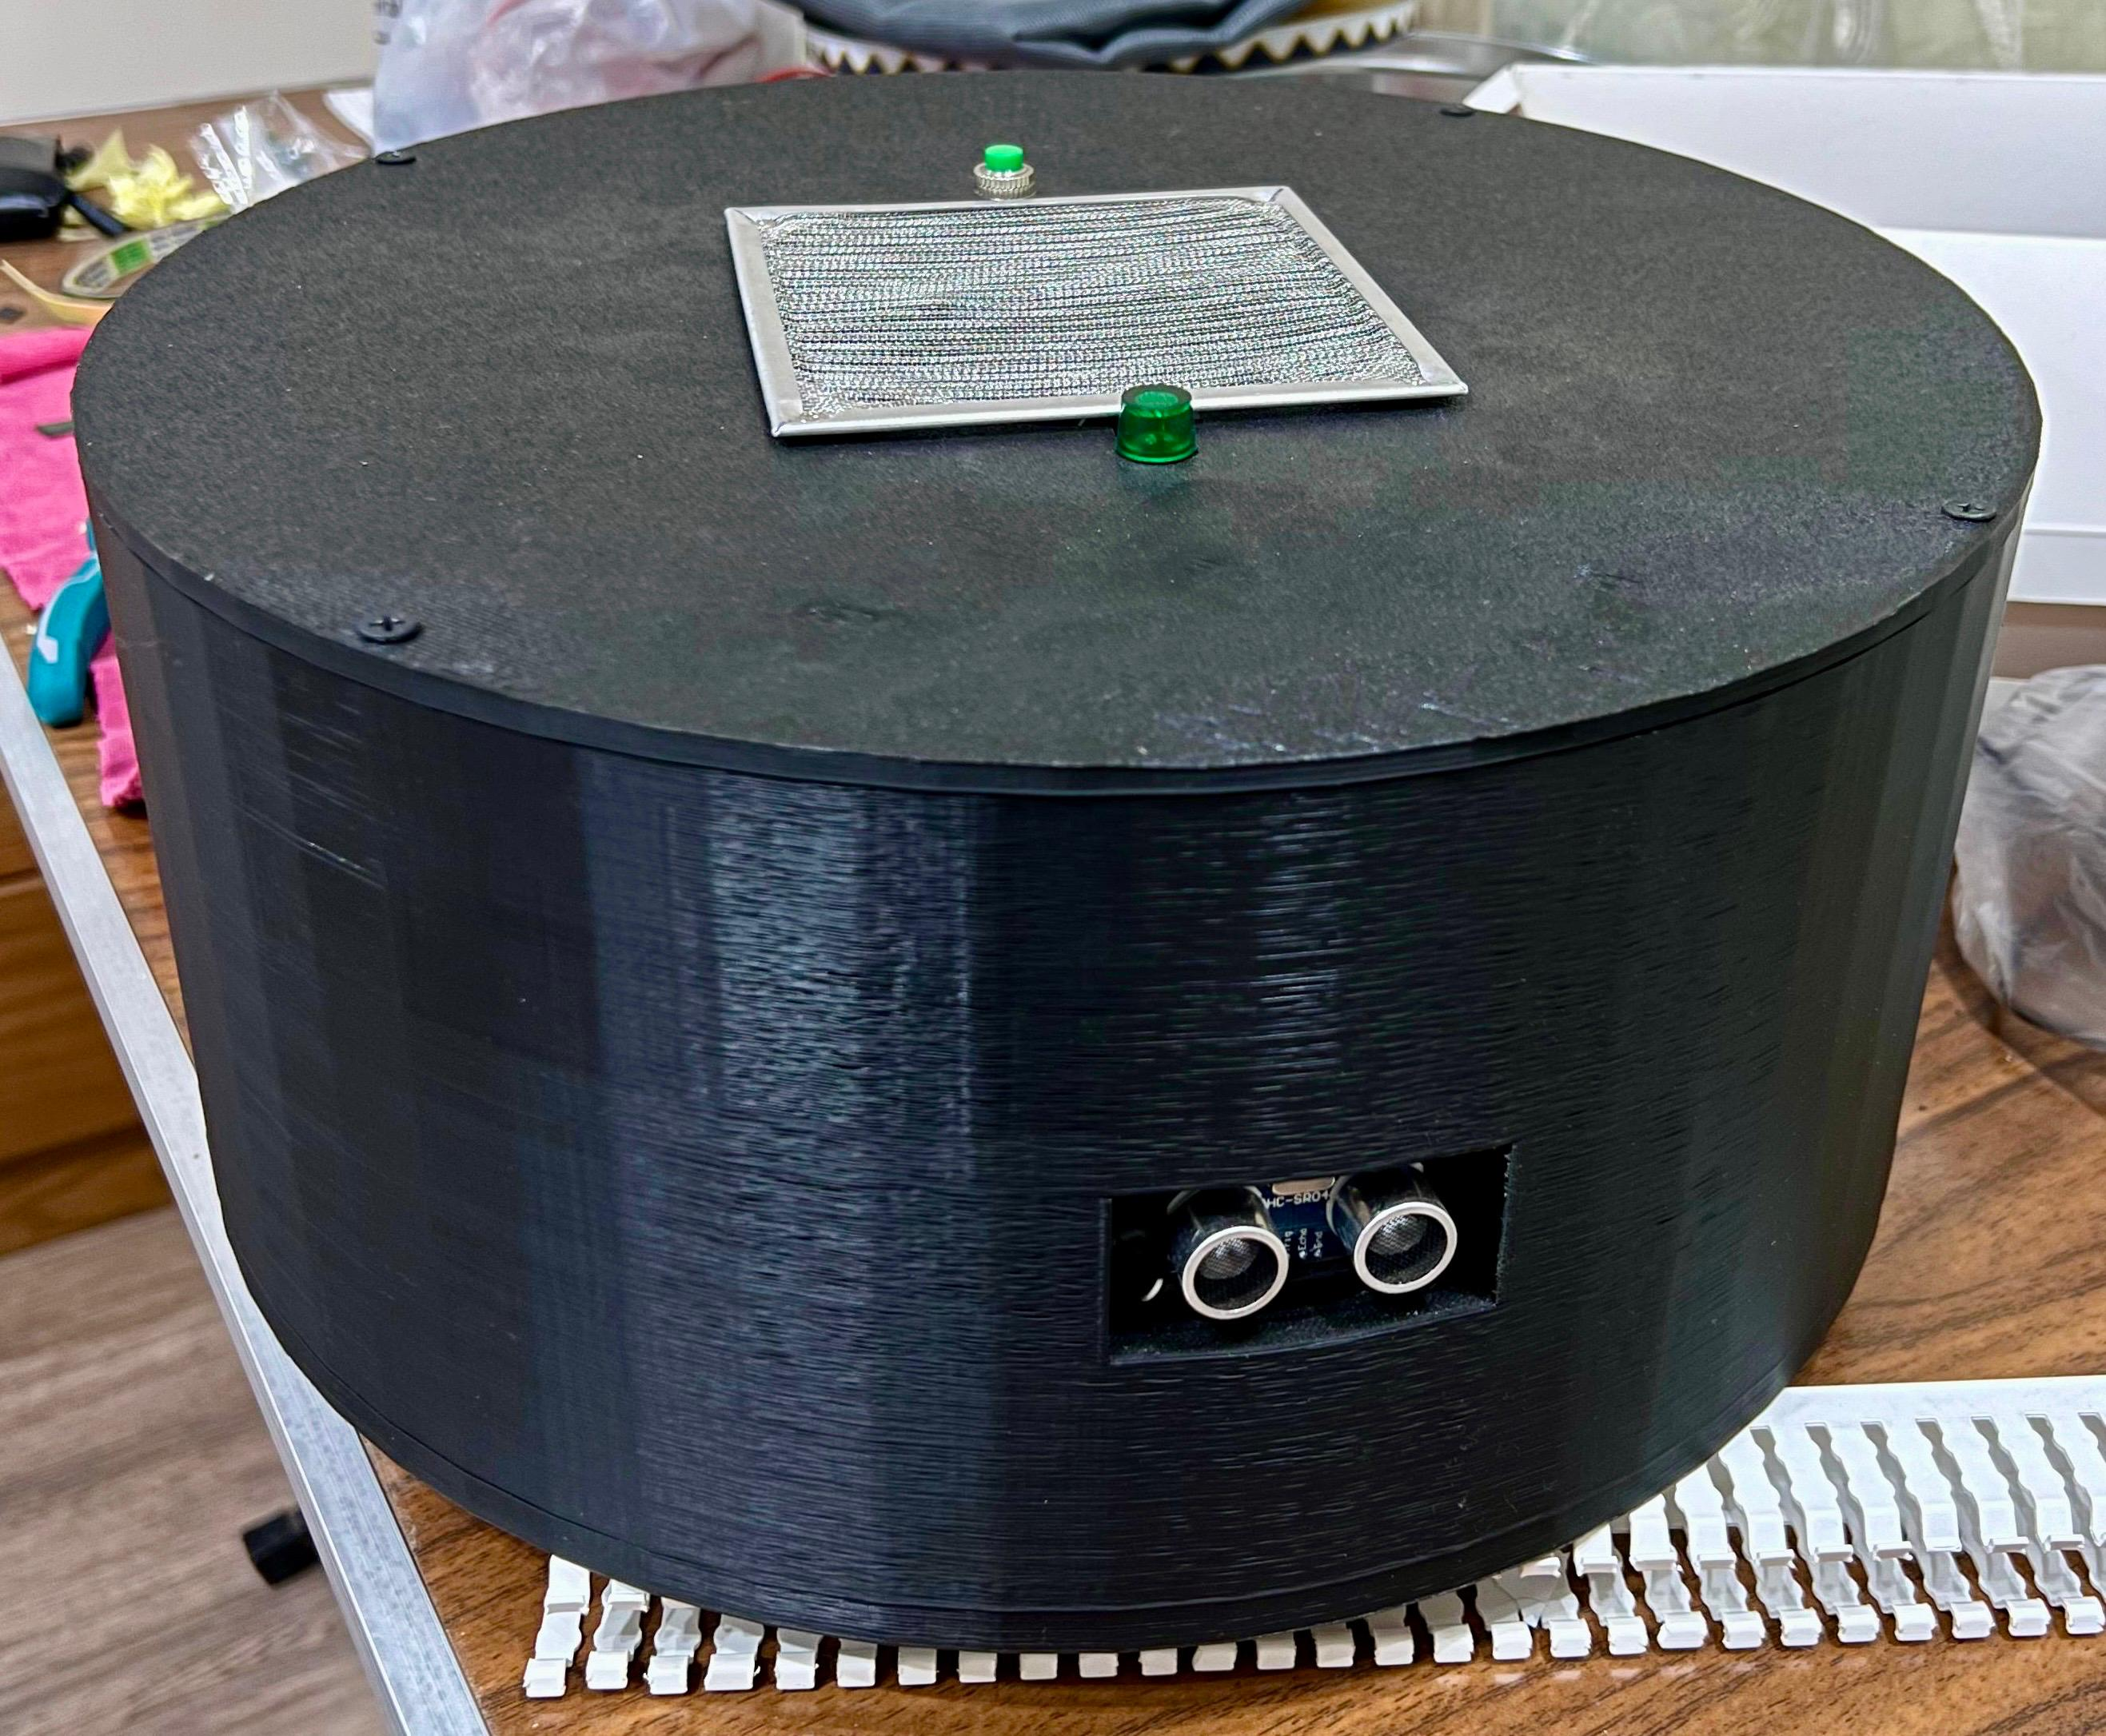
\includegraphics[width=\linewidth, keepaspectratio]{images/photos/robot_assembled_iso.jpg}
        \caption{Isometric view of the assembled robot.}
        \label{fig:assembled_robot_iso}
    \end{subfigure}
    \hfill % This adds some horizontal space between the images
    \begin{subfigure}[b]{0.496\textwidth}
        \centering
        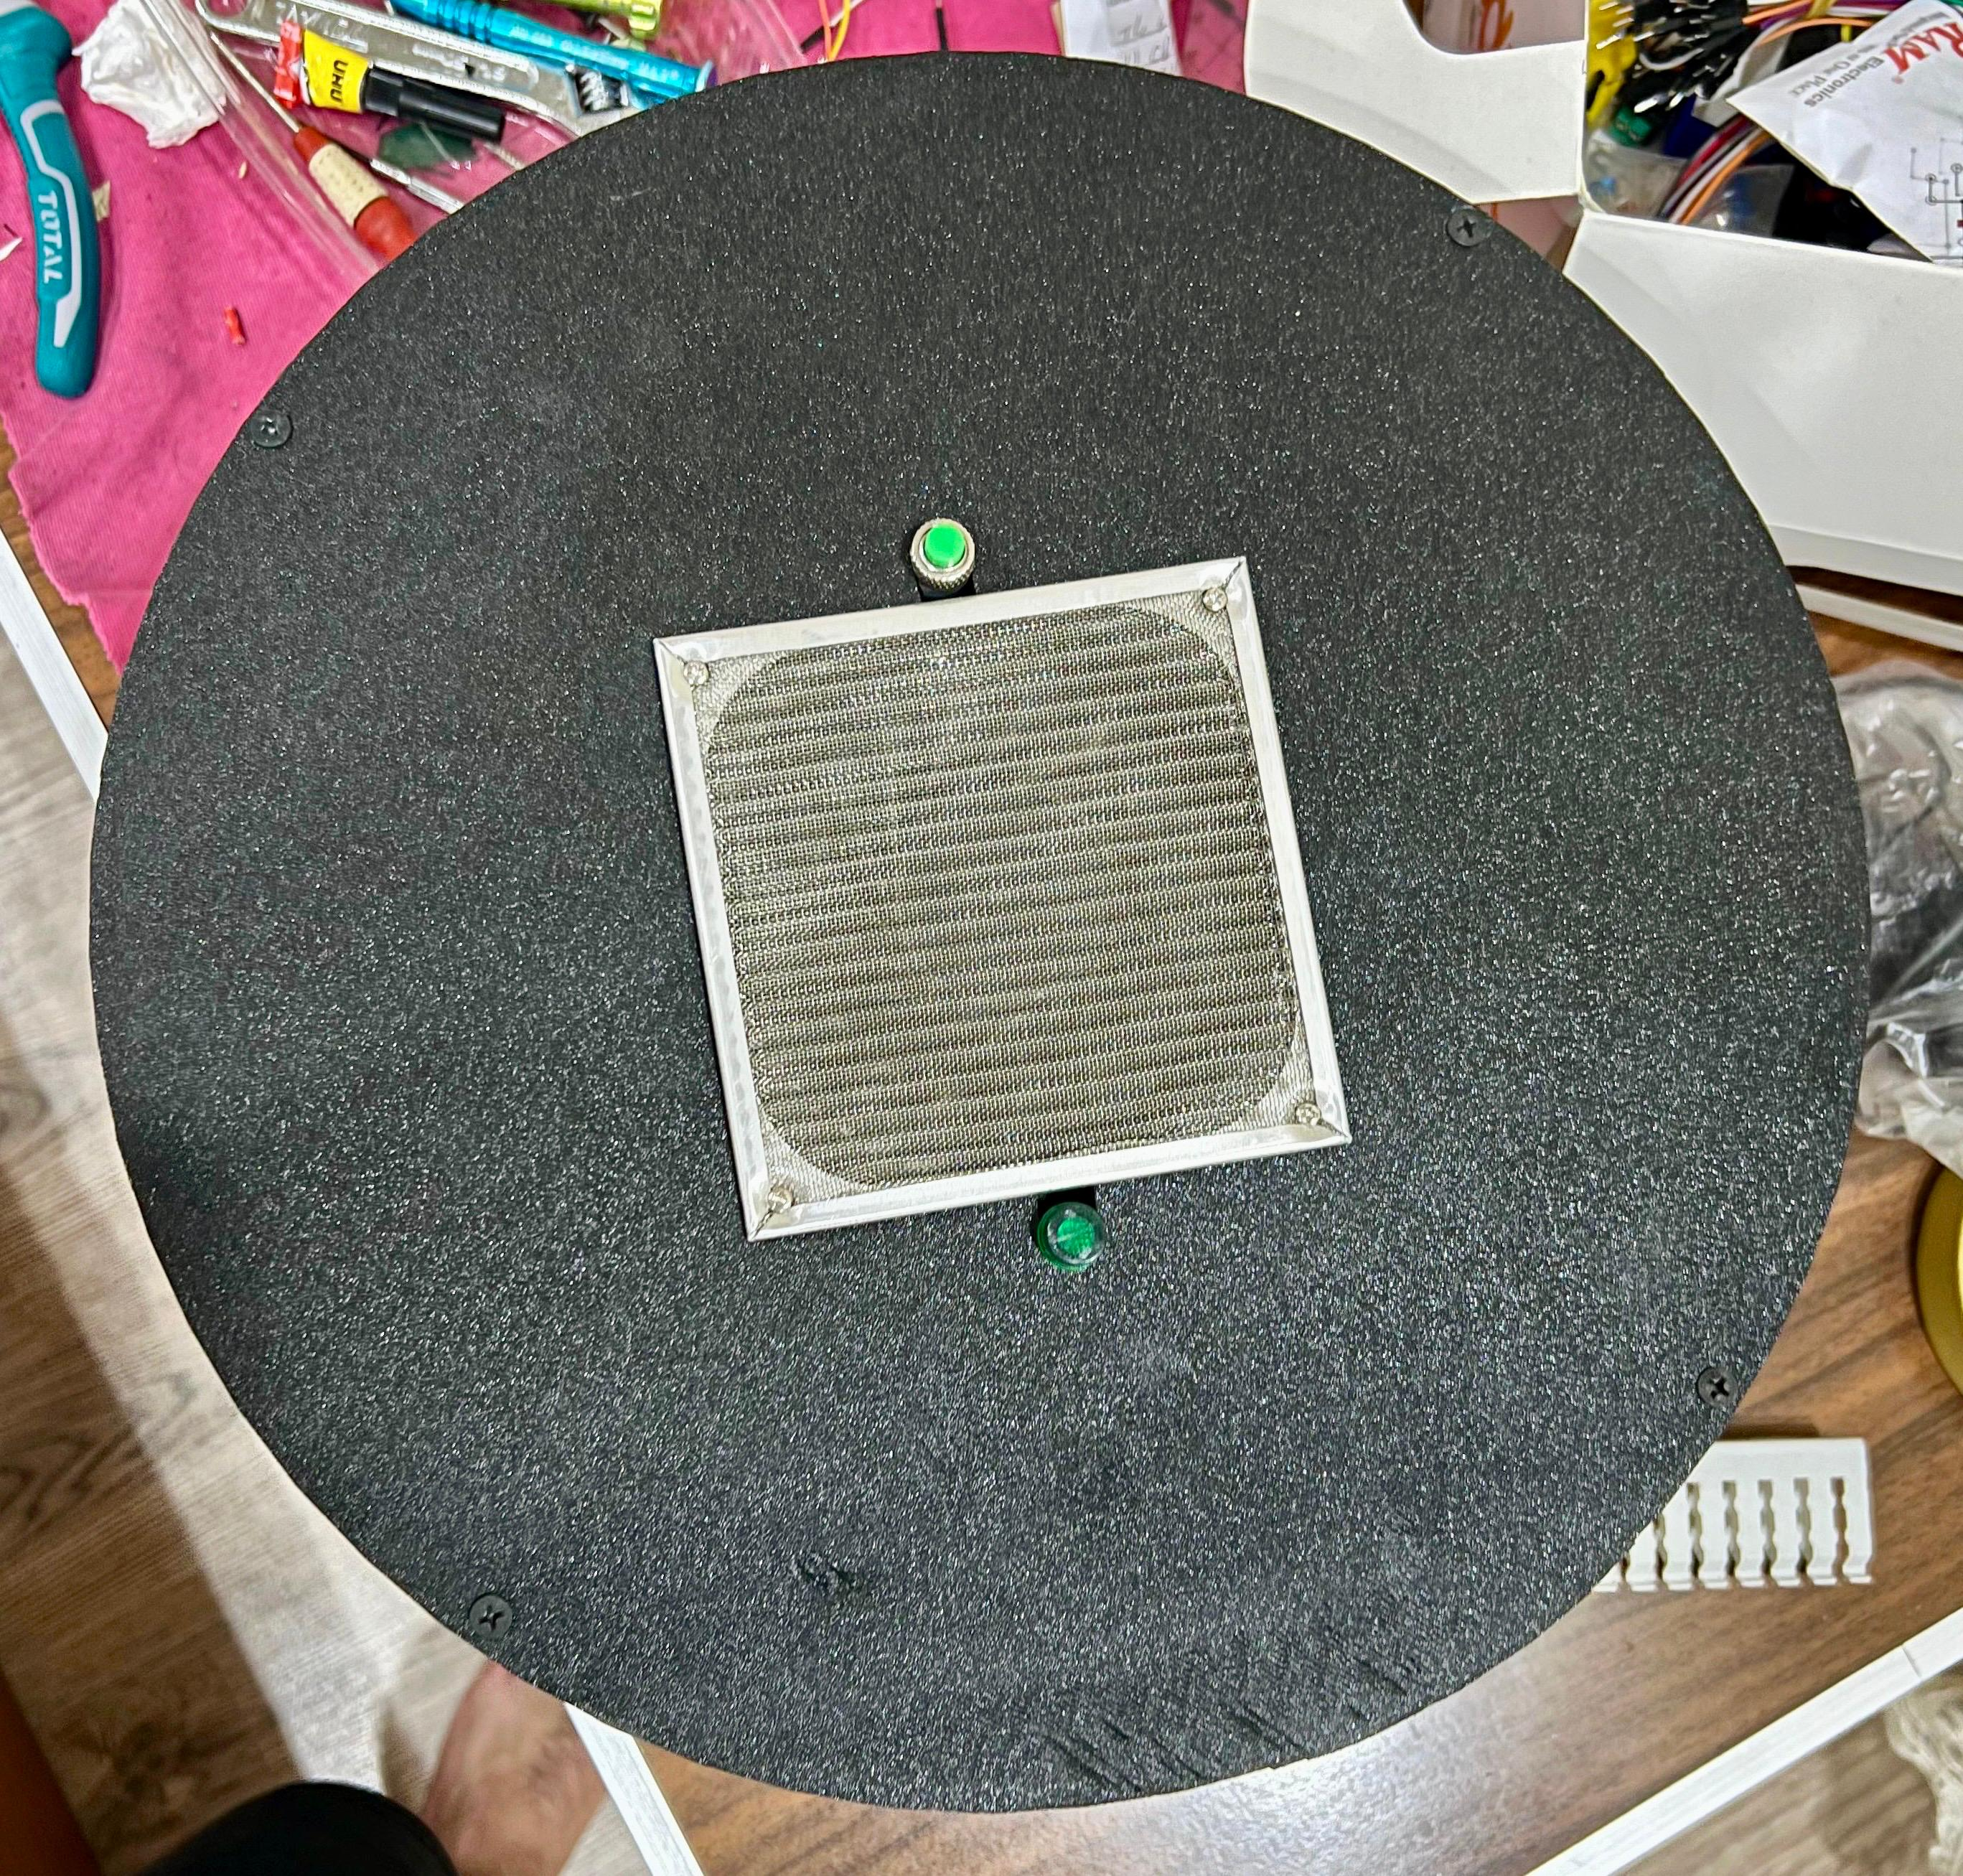
\includegraphics[width=\linewidth, keepaspectratio]{images/photos/robot_assembled_side.jpg}
        \caption{Top view of the assembled robot.}
        \label{fig:assembled_robot_side}
    \end{subfigure}
    \caption{Photographs of the 3D printed and assembled robot prototype.}
    \label{fig:assembled_robot_photos_eval_new}
\end{figure}
% --- NEW Chapter 4:Electrical and Control System Design and Testing ---
\chapter{Electrical and Control System Design and Testing}
\label{chap:electrical_control_performance} % New label for the combined chapter

\section{Introduction}
\label{sec:elec_control_intro}
This chapter details the electronic and software aspects of the Smart Cleaning Robot. It begins by outlining the key electrical components used and then describes the overall system architecture. The chapter then delves into the electrical design, including power distribution, component interconnections, and the custom \hyperref[term:pcb]{PCB} that forms the heart of the robot's electronics. Following this, the control system implementation is discussed, covering the MicroPython software developed for the Raspberry Pi Pico W, its architecture, navigation logic, and \hyperref[term:ble]{BLE} remote control capabilities. Finally, the chapter presents a qualitative performance evaluation of the fully assembled and programmed prototype.

\section{Electrical Components Summary}
\label{sec:electrical_components_summary}
The core electrical and electronic components enabling the robot's functionality are listed in Table~\ref{tab:electrical_components}. These components are responsible for power management, sensing, control, and actuation. A comprehensive Bill of Materials, including all components and associated costs, is available in Appendix \ref{app:bom}.

\begingroup
\small % Make font smaller for the table content
% Adjusted for 4 columns: Comp | Photo | Dims | Elec Specs
\sloppy % Allow more flexible spacing within the table
\renewcommand{\arraystretch}{1.2} % Add vertical padding
\begin{longtable}{|L{3.3cm}|p{1.9cm}|L{2.4cm}|L{5.4cm}|}
\caption{Electrical Components List} \label{tab:electrical_components} \\
\hline
\textbf{Component} & \textbf{Photo} & \textbf{Dimensions (cm)} & \textbf{Electrical Specifications} \\ \hline
\endfirsthead

\multicolumn{4}{c}%
{{\tablename\ \thetable\ -- \textit{Continued from previous page}}} \\
\hline
\textbf{Component} & \textbf{Photo} & \textbf{Dimensions (cm)} & \textbf{Electrical Specifications} \\ \hline
\endhead

% Footer with totals - CORRECTED ALIGNMENT
\hline 
\multicolumn{3}{|r|}{\cellcolor{lightgray}\textbf{System Voltage:}} & \multicolumn{1}{l|}{\cellcolor{lightgray}\totalVoltage} \\ \hline
\multicolumn{3}{|r|}{\cellcolor{lightgray}\textbf{Approx. Operational Current:}} & \multicolumn{1}{l|}{\cellcolor{lightgray}\totalCurrent} \\ \hline
\multicolumn{3}{|r|}{\cellcolor{lightgray}\textbf{Approx. Operational Power:}} & \multicolumn{1}{l|}{\cellcolor{lightgray}\totalPower} \\ \hline
\endlastfoot


% --- START OF ELECTRICAL COMPONENTS ---
\href{https://microohm-eg.com/product/raspberry-pi-pico-w-wireless-wh-with-soldered-headers/}{\textbf{\textcolor{darkblue}{Raspberry Pi Pico W}}}~\cite{PicoWDatasheet, RpiPicoWHProductPage} & 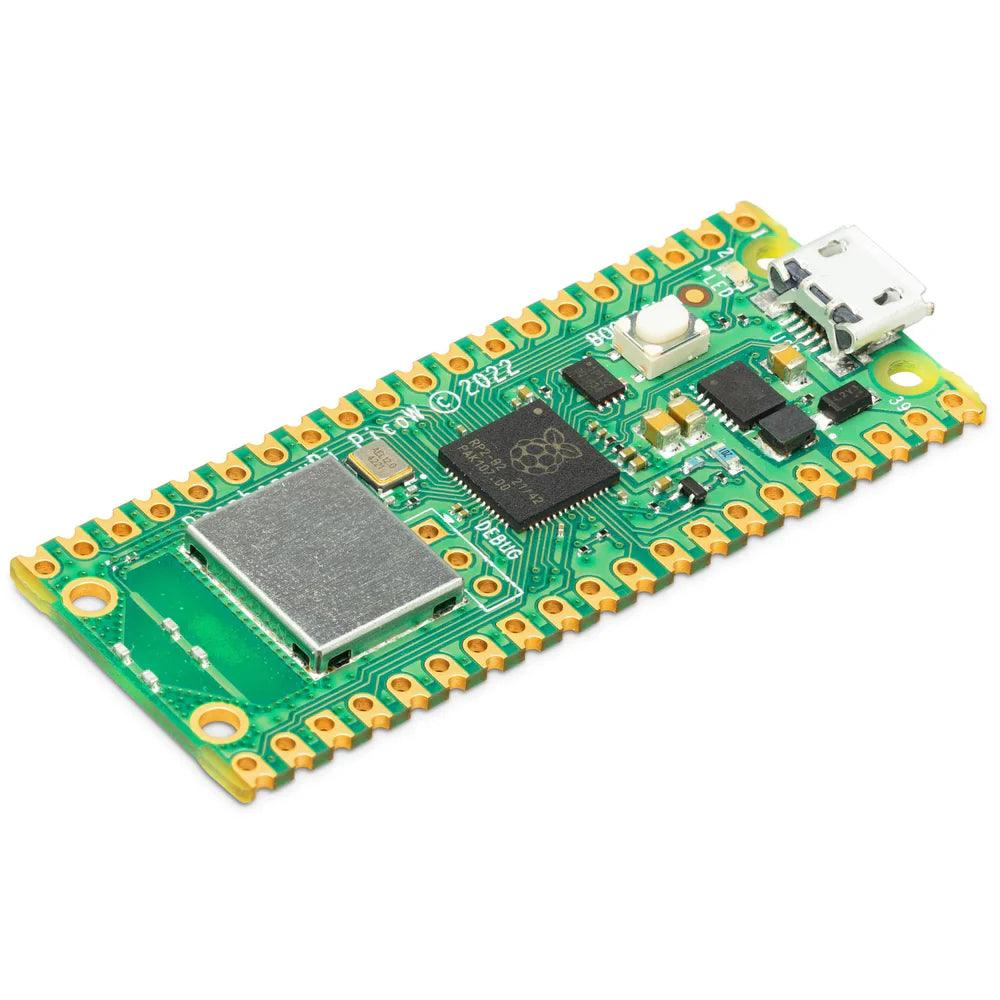
\includegraphics[width=\linewidth, keepaspectratio]{images/components/pico_w.jpg} & PCB: 2.1$\times$5.1 & RP2040, Dual-core ARM Cortex-M0+ @133MHz\newline \textbf{Voltage:} 1.8–5.5V, 3.3V logic\newline \textbf{Current:} ~91 mA (Wi-Fi active)\newline \textbf{Power:} Max ~0.5W \\ \hline

\href{https://www.ram-e-shop.com/shop/ro-motor-tt-mini-dc-gearbox-motors-pair-2-motors-with-back-shaft-9455}{\textbf{\textcolor{darkblue}{DC Motors (TT Mini Gearbox Pair)}}} & 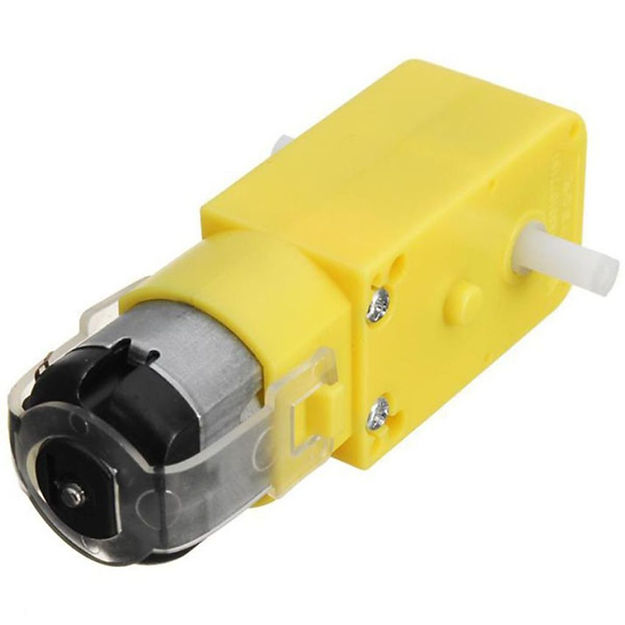
\includegraphics[width=\linewidth, keepaspectratio]{images/components/dc_motor_tt.jpg} & Per motor:\newline W2.2$ \newline \times$L7$\times$H1.8 & \textbf{No-load Speed:} 90 RPM\newline \textbf{Max Torque:} 800 gf.cm\newline \textbf{Voltage:} 3-12V\newline \textbf{No-load Current:} 190-250mA \\ \hline

\href{https://www.ram-e-shop.com/shop/kit-l298-red-l298-module-red-board-dual-h-bridge-motor-driver-using-l298n-7084}{\textbf{\textcolor{darkblue}{H-Bridge L298N Motor Driver}}}~\cite{L298NDatasheet, GeeetechL298NBoard} & 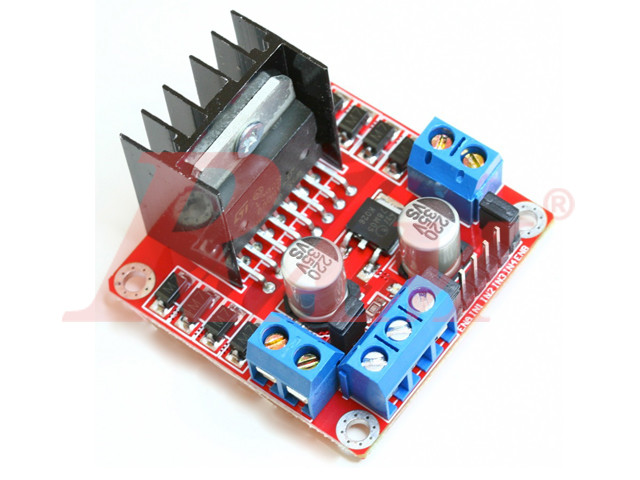
\includegraphics[width=\linewidth, keepaspectratio]{images/components/l298n_driver.jpg} & 4.3$\times$4.3$\times$2.7 & \textbf{Logic Voltage:} 5V\newline \textbf{Drive Voltage:} 5-35V\newline \textbf{Max Current:} 2A/channel\newline \textbf{Max Power:} 25W \\ \hline

\href{https://www.ram-e-shop.com/shop/kit-ultrasonic-hcsr04-ultrasonic-sensor-hc-sr04-5949}{\textbf{\textcolor{darkblue}{HC-SR04 Sensor}}}~\cite{HCSR04Datasheet} & 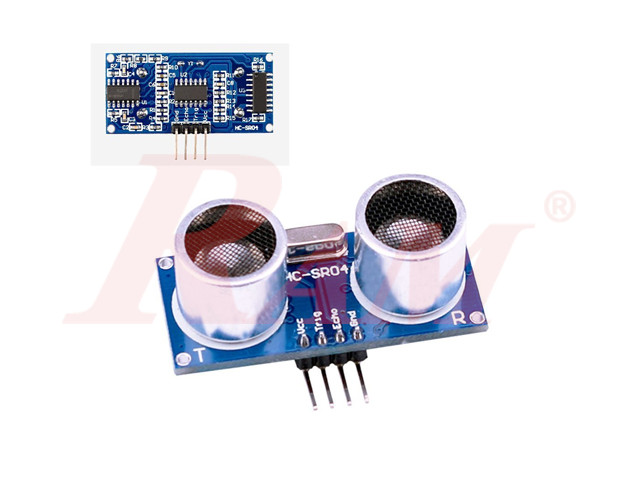
\includegraphics[width=\linewidth, keepaspectratio]{images/components/hcsr04_sensor.jpg} & W4.45 \newline $\times$H2$\times$D1.5 & \textbf{Voltage:} 5V DC\newline \textbf{Current:} $\sim$15mA\newline \textbf{Range:} 2cm - 400cm \\ \hline

\href{https://www.ram-e-shop.com/shop/battery-li-12v-4000mah-battery-pack-12v-4000mah-6728}{\textbf{\textcolor{darkblue}{Battery Pack}}}~\cite{BatteryPack12V4000mAhDatasheet} & 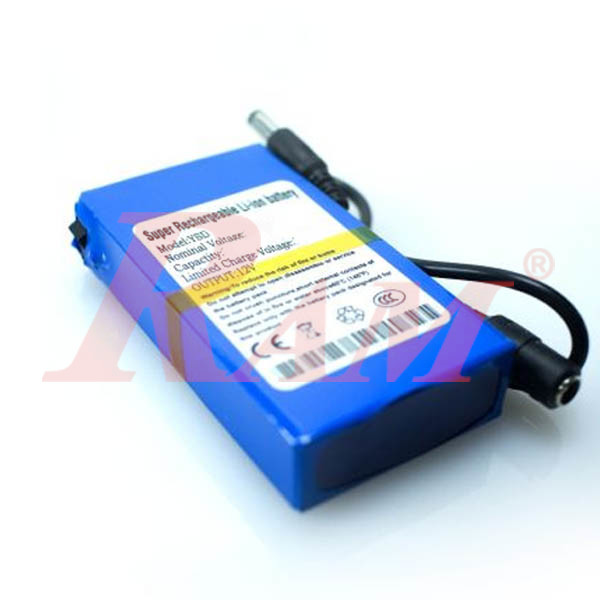
\includegraphics[width=\linewidth, keepaspectratio]{images/components/battery_12v.jpg} & 9.3$\times$6$\times$1.8 & \textbf{Output:} DC 2.1mm Jack\newline \textbf{Type:} \hyperref[term:liion]{Lithium-ion}\newline \textbf{Capacity:} 4000mAh @ 12V \\ \hline

\href{https://www.psdevwiki.com/ps3/Delta_KSB1012HE}{\textbf{\textcolor{darkblue}{PS3 Fan}}}~\cite{DeltaKSB1012HE_PSDevWiki} & 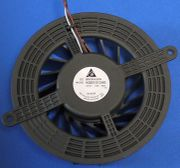
\includegraphics[width=\linewidth, keepaspectratio]{images/components/ps3_fan.jpg} & Diameter: $\sim$10 & \textbf{Voltage:} 12V DC\newline \textbf{Current:} $\sim$1.30A\newline \textbf{Connection:} 3-Pin (Pwr, Gnd, PWM Ctrl) \\ \hline

\href{https://www.ram-e-shop.com/shop/dc-dc-100-dc-dc-step-down-voltage-converter-adjustable-3a-lm2596s-4-38vdc-to-1-5-35vdc-sku-dc100-7257}{\textbf{\textcolor{darkblue}{DC-DC Step Down LM2596S}}}~\cite{LM2596SDatasheet} & 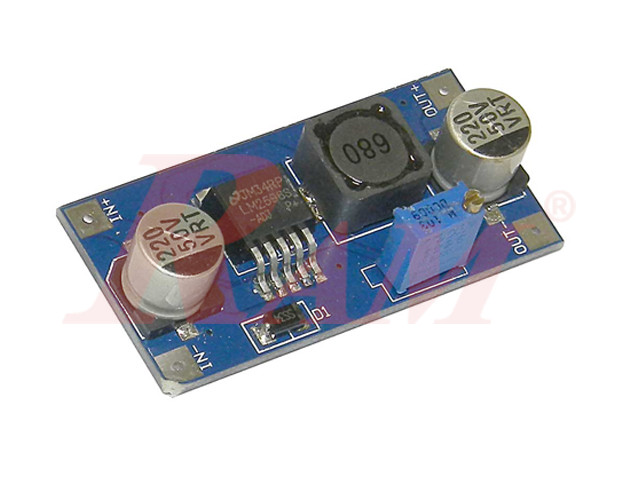
\includegraphics[width=\linewidth, keepaspectratio]{images/components/lm2596s_buck.jpg} & 4.35$\times$2.1$\times$1.4 & \textbf{Input:} 4-38V DC\newline \textbf{Output:} 1.5-35V DC (Adj.)\newline \textbf{Current:} 3A Max\newline \textbf{Frequency:} 150kHz \\ \hline

\href{https://homesensors.net/product/ir-photoelectric-encoder-sensor-4pin/}{\textbf{\textcolor{darkblue}{IR Photoelectric Encoder Sensor}}} & 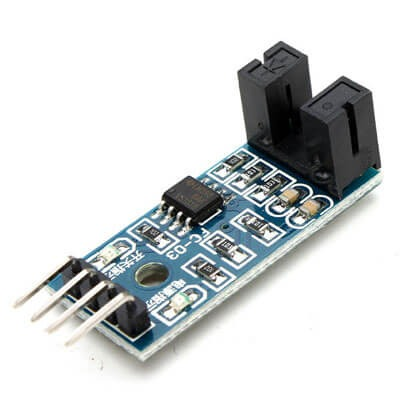
\includegraphics[width=\linewidth, keepaspectratio]{images/components/encoder_sensor.jpg} & 3.2$\times$1.4$\times$1.0 & \textbf{IC:} LM393\newline \textbf{Voltage:} 3.3-5.0V\newline \textbf{Groove Width:} 5mm\newline \textbf{Output:} Digital TTL \\ \hline

\href{https://homesensors.net/product/rotary-encoder-1pcs/}{\textbf{\textcolor{darkblue}{Rotary Encoder Disc}}} & 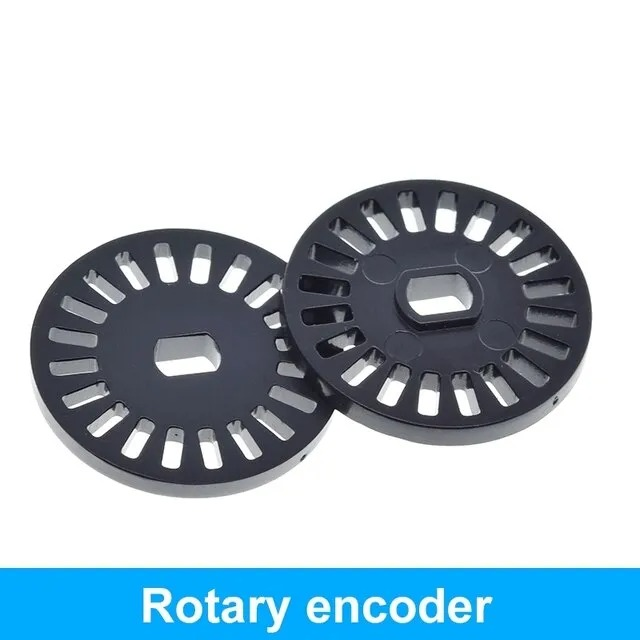
\includegraphics[width=\linewidth, keepaspectratio]{images/components/encoder_disc.jpg} & $\varnothing$: ~2.5 & \textbf{Material:} Plastic\newline \textbf{Slots:} 20 \\ \hline

\href{https://www.ram-e-shop.com/shop/pb-2-green-push-button-type-2-green-color-5614}{\textbf{\textcolor{darkblue}{Push Button (Green)}}} & 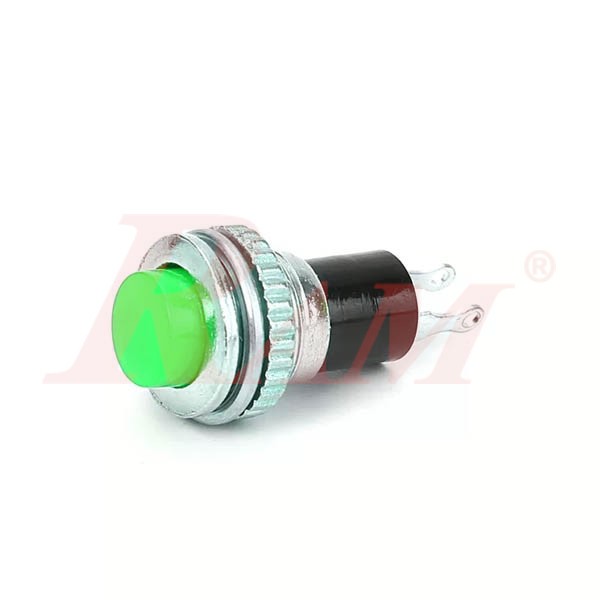
\includegraphics[width=\linewidth, keepaspectratio]{images/components/push_button_green.jpg} & Thread $\varnothing$: 9mm\newline Button $\varnothing$: 7mm\newline Overall: 1.2$\times$2.5 & \textbf{Type:} Momentary, Normally Open\newline \textbf{Rating:} AC 3A/125V, 1.5A/250V \\ \hline

\href{https://www.ram-e-shop.com/shop/xd10-3-12vdc-green-xd10-3-dc12v-green-small-led-signal-indicator-light-10mm-9155}{\textbf{\textcolor{darkblue}{LED Indicator}}} & 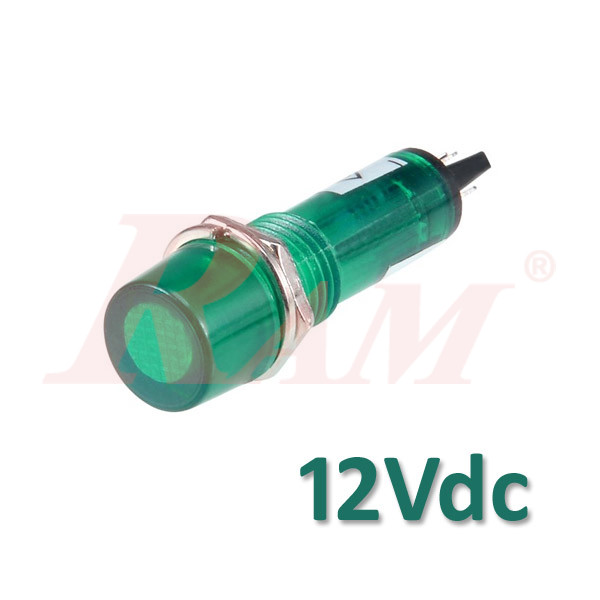
\includegraphics[width=\linewidth, keepaspectratio]{images/components/led_indicator.jpg} & Mount Hole $\varnothing$: 10mm\newline Overall: L4.15$\times\varnothing$1.15 & \textbf{Rated Voltage:} DC 12V\newline \textbf{Color:} Green \\ \hline

\href{https://www.ram-e-shop.com/shop/r-5-roseta-2pin-2-pin-pcb-screw-terminal-block-pitch-5mm-14-1mm-long-r-5-6323}{\textbf{\textcolor{darkblue}{2 Pin Screw Terminal}}} & 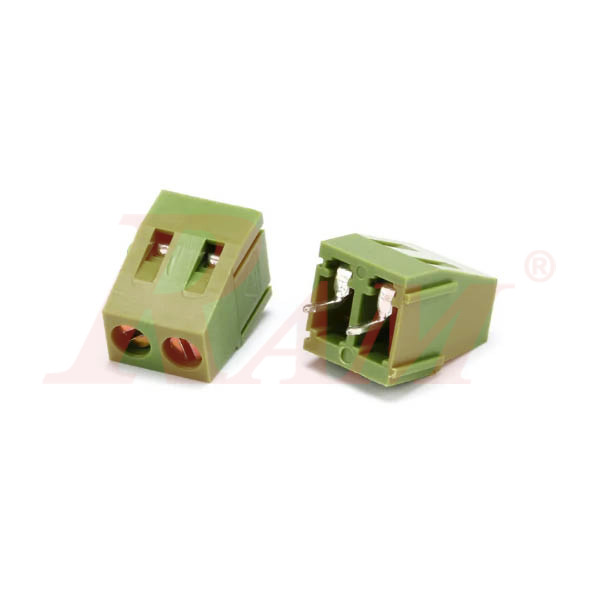
\includegraphics[width=\linewidth, keepaspectratio]{images/components/terminal_2pin.jpg} & Pitch: 0.5\newline Pin Dim: 0.43 & \textbf{Rating:} 24A / 250V\newline \textbf{Wire:} 26-14AWG \\ \hline

\href{https://www.ram-e-shop.com/shop/r-6-roseta-3pin-3-pin-pcb-screw-terminal-block-pitch-5mm-14-1mm-long-r-6-6322}{\textbf{\textcolor{darkblue}{3 Pin Screw Terminal}}} & 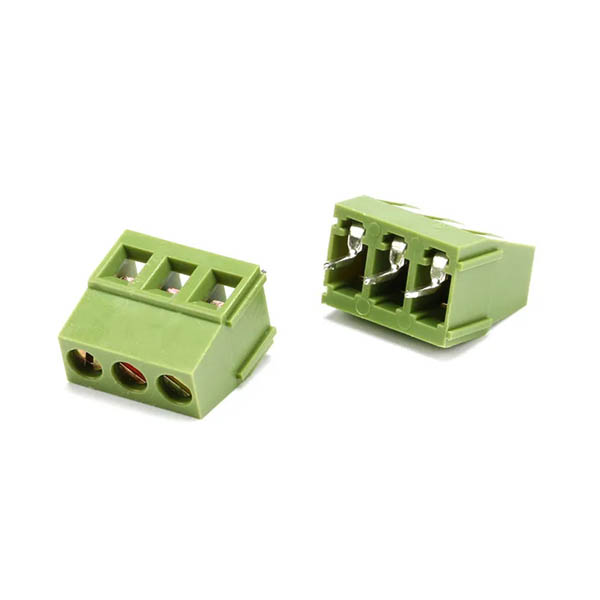
\includegraphics[width=\linewidth, keepaspectratio]{images/components/terminal_3pin.jpg} & Pitch: 0.5\newline Pin Dim: 0.43 & \textbf{Rating:} 24A / 250V\newline \textbf{Wire:} 26-14AWG \\ \hline

\href{https://www.ram-e-shop.com/shop/ph35-1x20-female-ph35-pin-header-female-1x20-straight-2-54mm-6529}{\textbf{\textcolor{darkblue}{Pin Header Female 1x20}}} & 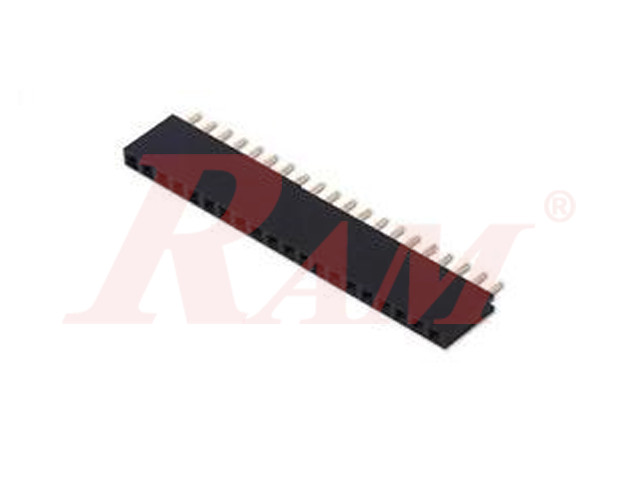
\includegraphics[width=\linewidth, keepaspectratio]{images/components/pin_header_female.jpg} & Spacing: 0.254 & \textbf{Configuration:} 1x20 Pins, Straight\newline \textbf{Current Rating:} 3A \\ \hline

\href{https://microohm-eg.com/product/6mm-electrical-waterproof-seal-heat-shrink-splice-wire-sleeve-yellow-1pcs/}{\textbf{\textcolor{darkblue}{Heat Shrink Sleeve (6mm Yellow)}}} & 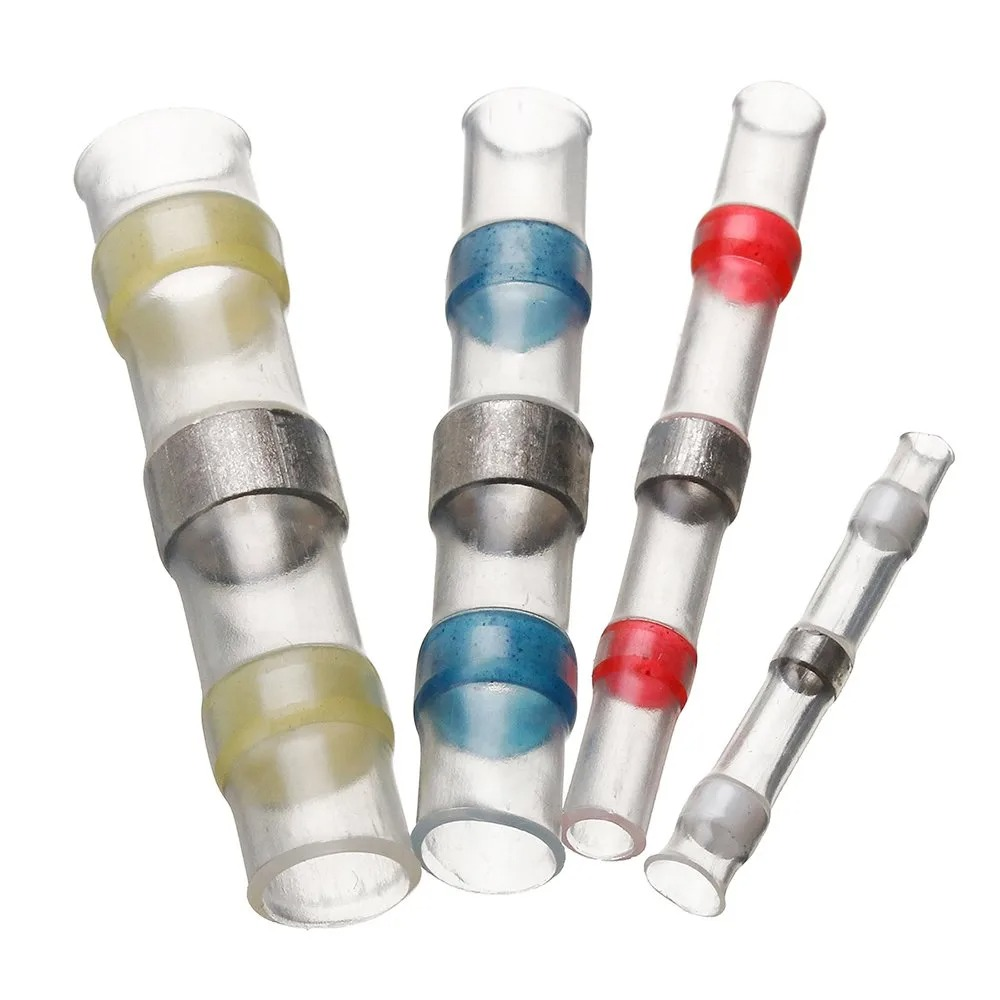
\includegraphics[width=\linewidth, keepaspectratio]{images/components/heat_shrink.jpg} & $\varnothing$: 0.6\newline Length: 4.0 & \textbf{Material:} Polyolefin\newline \textbf{Shrink Ratio:} 2:1, Waterproof \\ \hline

{\textbf{\textcolor{darkblue}{Resistor 2.2k$\Omega$}}} & 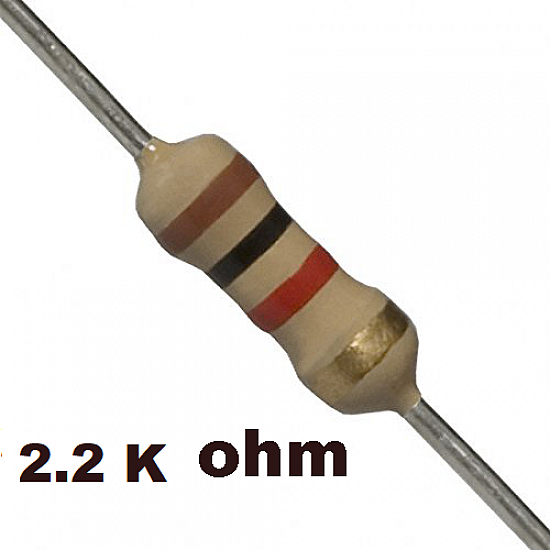
\includegraphics[width=\linewidth, keepaspectratio]{images/components/resistor_2k2.png} & Axial Pkg. & \textbf{Value:} 2.2k$\Omega$\newline \textbf{Power:} 1/4W\newline \textbf{Type:} Axial \\ \hline

{\textbf{\textcolor{darkblue}{Resistor 4.7k$\Omega$}}} & 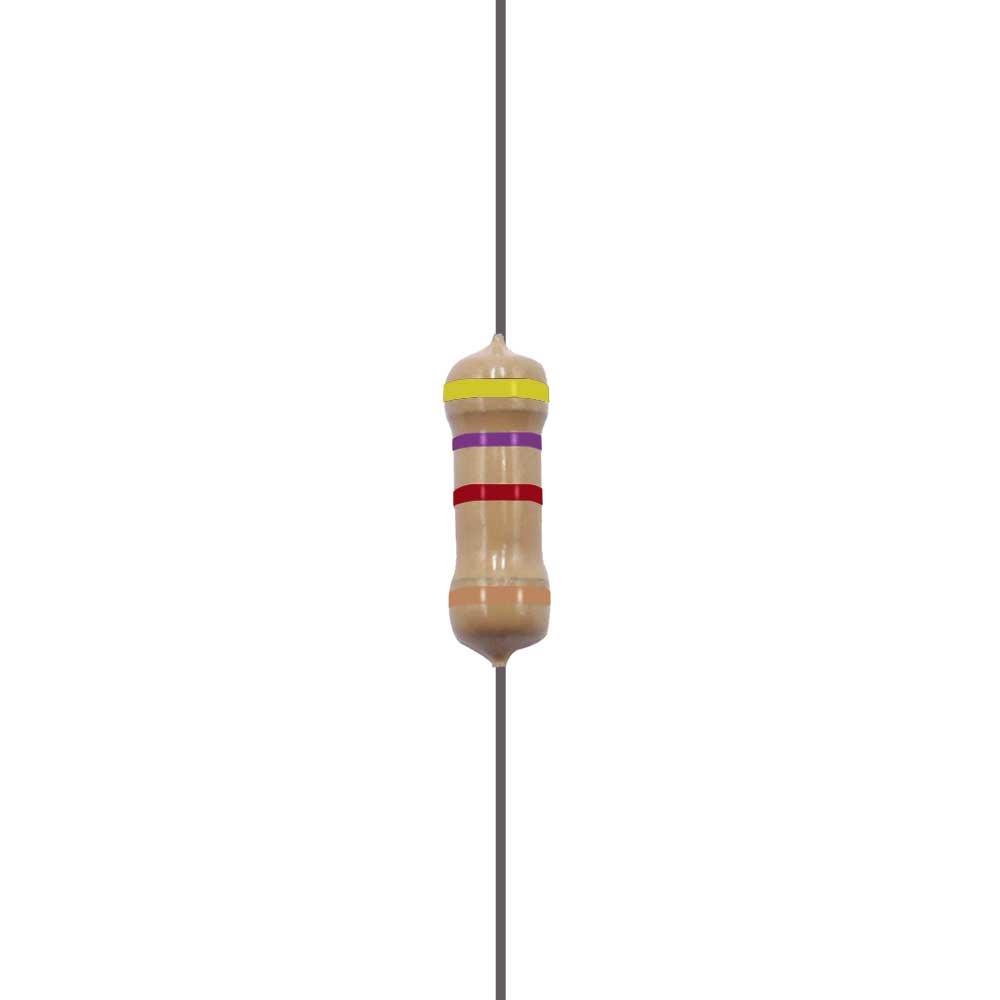
\includegraphics[width=\linewidth, keepaspectratio]{images/components/resistor_4k7.jpg} & Axial Pkg. & \textbf{Value:} 4.7k$\Omega$\newline \textbf{Power:} 1/4W\newline \textbf{Type:} Axial \\ \hline

\href{https://www.ram-e-shop.com/shop/ph60-mf-20cm-ph60-20cm-male-to-female-40-jumper-wires-set-7066}{\textbf{\textcolor{darkblue}{Jumper Wires M-F}}} & 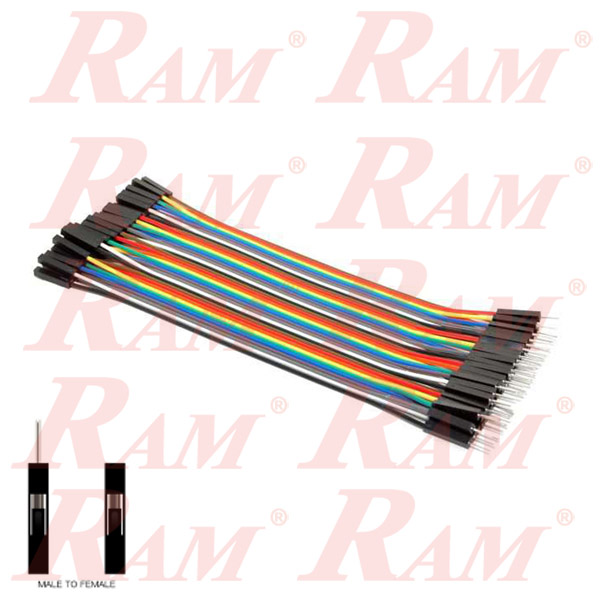
\includegraphics[width=\linewidth, keepaspectratio]{images/components/jumper_mf.jpg} & Length: 20 & \textbf{Configuration:} Male-to-Female\newline \textbf{Quantity:} 40 Wires\newline \textbf{Current Rating:} 1A \\ \hline

\href{https://www.ram-e-shop.com/shop/ph61-mm-20cm-ph61-20cm-male-to-male-40-jumper-wires-set-7094}{\textbf{\textcolor{darkblue}{Jumper Wires M-M}}} & 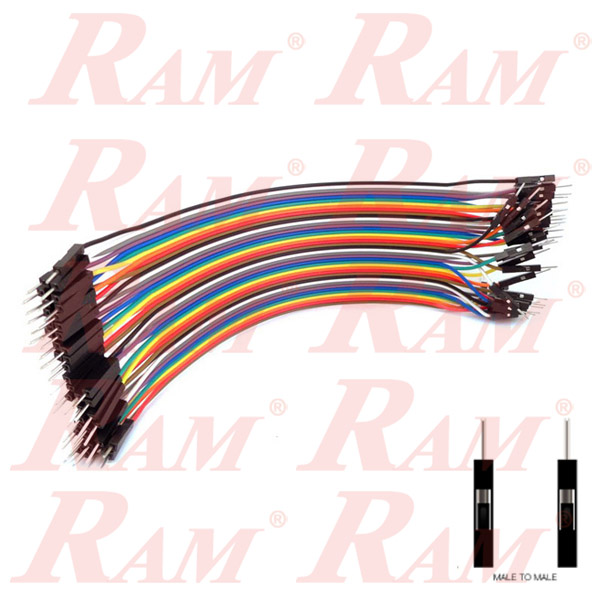
\includegraphics[width=\linewidth, keepaspectratio]{images/components/jumper_mm.jpg} & Length: 20 & \textbf{Configuration:} Male-to-Male\newline \textbf{Quantity:} 40 Wires\newline \textbf{Current Rating:} 1A \\ \hline

\href{https://www.ram-e-shop.com/shop/ph62-ff-20cm-ph62-20cm-female-to-female-40-jumper-wires-set-7189}{\textbf{\textcolor{darkblue}{Jumper Wires F-F}}} & 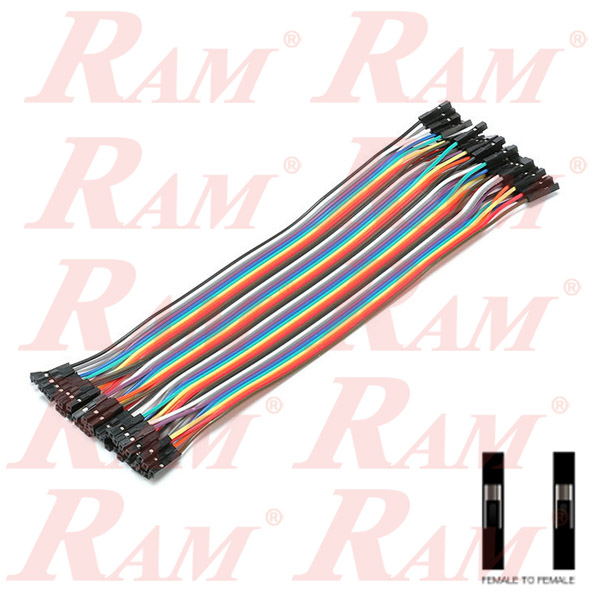
\includegraphics[width=\linewidth, keepaspectratio]{images/components/jumper_ff.jpg} & Length: 20 & \textbf{Configuration:} Female-to-Female\newline \textbf{Quantity:} 40 Wires\newline \textbf{Current Rating:} 1A \\ \hline

\href{https://www.ram-e-shop.com/shop/wire-speaker-2x1mm-speaker-wire-2-core-x-1mm-red-black-1-meter-8878}{\textbf{\textcolor{darkblue}{Speaker Wire}}} & 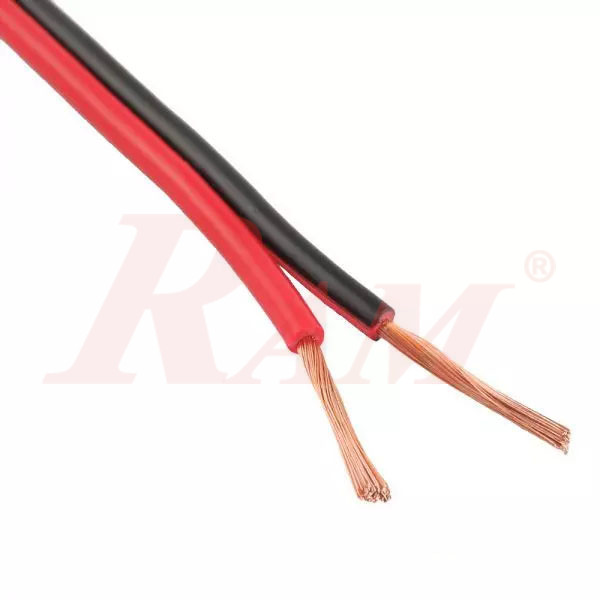
\includegraphics[width=\linewidth, keepaspectratio]{images/components/speaker_wire.jpg} & Size: 2Cx0.1\newline Length: 100 (per meter) & \textbf{Colors:} Red \& Black\newline \textbf{Material:} OFC Copper, PVC Jacket \\ \hline

\end{longtable}
\fussy % Return to normal spacing behavior after the table
\endgroup

\section{System Architecture}
\label{sec:system_architecture_ctrl_new} % Relabelled from old sec:system_architecture_ctrl
The robot's control system is centralized around the Raspberry Pi Pico W microcontroller~\cite{PicoWDatasheet}. This board was chosen for its dual-core ARM Cortex-M0+ processor, sufficient \hyperref[term:gpio]{GPIO} pins, integrated Wi-Fi and \hyperref[term:ble]{BLE} capabilities (Pico W variant), low cost, and robust MicroPython support~\cite{RpiPicoSeriesDocs}. A pinout diagram for the Raspberry Pi Pico W is shown in Figure~\ref{fig:pico_w_pinout_diagram_new}. The Pico W is responsible for:
\begin{itemize}
    \item Reading and processing data from the \hyperref[term:hcsr04]{HC-SR04} ultrasonic sensor for obstacle detection.
    \item Processing high-frequency interrupt signals from two wheel encoders for odometry.
    \item Controlling the two \hyperref[term:dc]{DC} gear motors via an \hyperref[term:l298n]{L298N} H-bridge motor driver, using a \hyperref[term:pid]{PID} algorithm for precise motion control.
    \item Managing the operation of the 12V PS3 fan.
    \item Handling user input from a physical start/stop button.
    \item Providing status feedback via an \hyperref[term:led]{LED} indicator.
    \item Managing \hyperref[term:ble]{BLE} communication for remote control via a smartphone application like NRF Toolbox.
\end{itemize}

Figure~\ref{fig:system_block_diagram} provides a high-level overview of the autonomous cleaning control flow, illustrating how the system transitions between user commands, forward motion with hybrid feed-forward and PID control, obstacle detection, and stall recovery.

\begin{figure}[htbp]
\centering
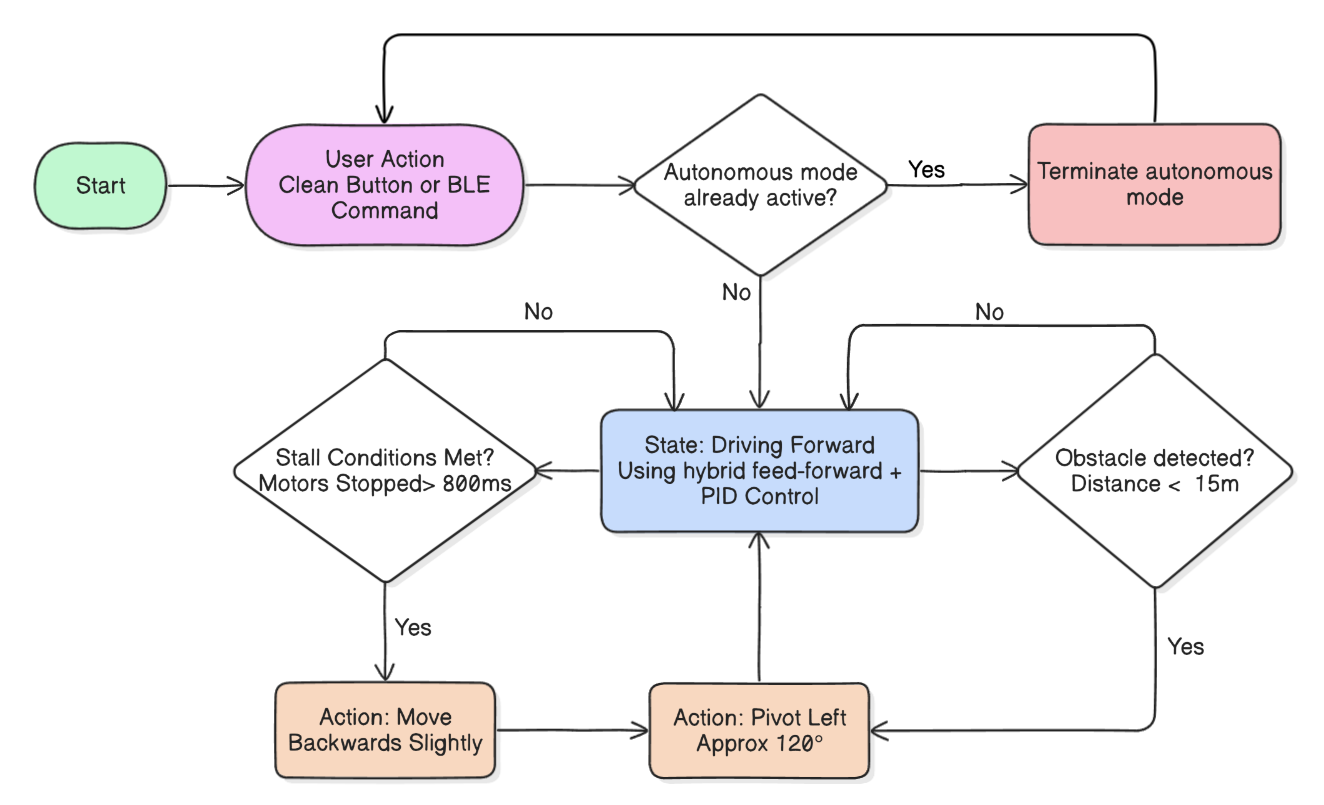
\includegraphics[width=\textwidth]{images/screenshots/control_flowchart.png}
\caption{High-level control flowchart of the autonomous cleaning mode, showing user-initiated activation, forward motion with hybrid PID control, obstacle avoidance, and stall recovery paths.}
\label{fig:system_block_diagram}
\end{figure}

\begin{sidewaysfigure}
    \centering
    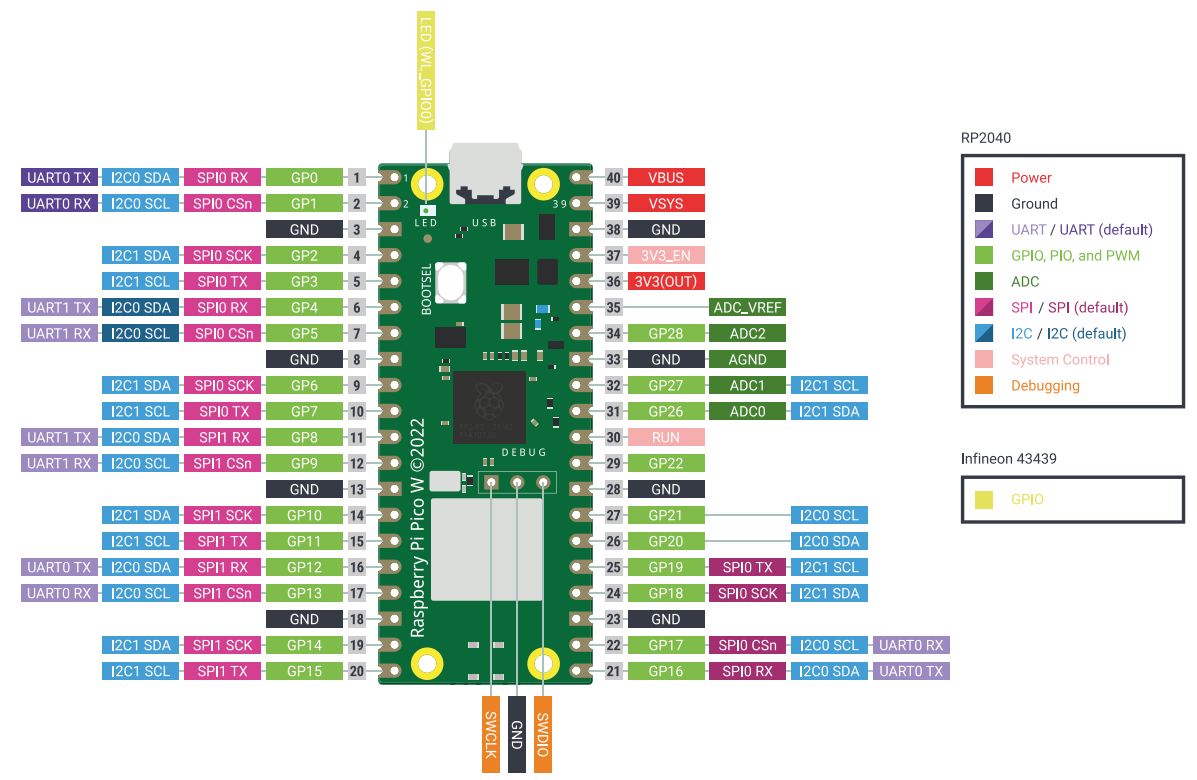
\includegraphics[width=1\textwidth, keepaspectratio]{images/screenshots/pico_w_pinout.png}
    \caption{Raspberry Pi Pico W pinout diagram. Source:~\cite{PicoWDatasheet}.}
    \label{fig:pico_w_pinout_diagram_new} % Relabelled from fig:pico_w_pinout_diagram
\end{sidewaysfigure}


\section{Electrical Design and Integration}
\label{sec:electrical_design_integration_new}
The electrical design focuses on safely and reliably interconnecting all electronic components, culminating in a custom \hyperref[term:pcb]{PCB} for a robust final assembly.
\subsection{Power Distribution}
\label{subsec:power_distribution_new}
\begin{itemize}
    \item The 12V \hyperref[term:liion]{Li-ion} battery~\cite{BatteryPack12V4000mAhDatasheet} is the primary power source.
    \item The LM2596S buck converter~\cite{LM2596SDatasheet} steps down the 12V to a regulated 5V. This 5V rail powers:
        \begin{itemize}
            \item The Raspberry Pi Pico W via its VSYS pin.
            \item The logic side of the \hyperref[term:l298n]{L298N} motor driver (Vss or +5V pin).
            \item The \hyperref[term:hcsr04]{HC-SR04} ultrasonic sensor (VCC pin).
            \item The two IR photoelectric encoder sensors (VCC pins).
        \end{itemize}
    \item The 12V from the battery directly powers:
        \begin{itemize}
            \item The motor input (Vs or VM) of the \hyperref[term:l298n]{L298N} module.
            \item The PS3 fan.
        \end{itemize}
    \item A common ground (GND) is maintained across all components.
\end{itemize}

\subsection{Component Interconnections and Wiring}
\label{subsec:component_interconnections_wiring_new}
The Raspberry Pi Pico W’s \hyperref[term:gpio]{GPIO} pins are used for all control signals and sensor inputs. Key connections are detailed in the accompanying MicroPython source code (\texttt{main.py}) and visualized in the schematic diagrams (see Section~\ref{subsec:custom_pcb_design_new}). The specific \hyperref[term:gpio]{GPIO} assignments are as follows:

\begin{itemize}
    \item \textbf{Motor Control (\hyperref[term:l298n]{L298N})}: Six \hyperref[term:gpio]{GPIO} pins from the Pico W control the \hyperref[term:l298n]{L298N} driver~\cite{L298NDatasheet}:
        \begin{itemize}
            \item Left Motor PWM (ENA): GP6
            \item Left Motor Direction 1 (IN1): GP12
            \item Left Motor Direction 2 (IN2): GP13
            \item Right Motor PWM (ENB): GP7
            \item Right Motor Direction 1 (IN3): GP14
            \item Right Motor Direction 2 (IN4): GP15
        \end{itemize}

    
    \item \textbf{Wheel Encoder Inputs}: To facilitate the closed-loop control system, the wheel encoders were connected directly to interrupt-capable GPIO pins:
        \begin{itemize}
            \item Left Encoder Sensor: GP21
            \item Right Encoder Sensor: GP20
        \end{itemize}
        These pins were configured with internal pull-ups in the software to ensure a stable signal.
    \item \textbf{Ultrasonic Sensor (\hyperref[term:hcsr04]{HC-SR04})}:
        \begin{itemize}
            \item TRIG (Output): GP10
            \item ECHO (Input): GP11
        \end{itemize}
        A voltage divider circuit (e.g., 2.2k$\Omega$ and 4.7k$\Omega$ resistors) is used on the ECHO pin to safely step down the sensor’s 5V output to the Pico W’s 3.3V logic level.
    \item \textbf{PS3 Fan}: The fan’s \hyperref[term:pwm]{PWM} control pin (Grey wire) is connected to GP8 on the Pico W. While this hardware connection could support future software-based \hyperref[term:pwm]{PWM} speed control, the current prototype implements simple on/off control using this pin (leaving software-based speed control as a potential future enhancement). The fan’s +12V (Brown) and GND (Black) wires are connected to the 12V power supply.
    \item \textbf{User Interface}:
        \begin{itemize}
            \item Push Button (Start/Stop): GP16 (configured with an internal pull-up resistor).
            \item \hyperref[term:led]{LED} Indicator: GP18 (connected via a suitable current-limiting resistor as required).
        \end{itemize}
\end{itemize}


Initial conceptual validation of the control logic, particularly for obstacle avoidance, was performed using Proteus simulation (Figure~\ref{fig:combined_sim_breadboard}(a)). An Arduino Uno model was employed in the simulation due to the unavailability of a Raspberry Pi Pico W model in Proteus at the time of testing; this allowed for early verification of the fundamental sensor-driven decision-making processes. Following this simulation-based logic testing, the actual electrical connections for the chosen components were physically validated on a breadboard (Figure~\ref{fig:combined_sim_breadboard}(b)) before committing to the \hyperref[term:pcb]{PCB} design.
\begin{figure}[htbp]
    \centering
    \begin{subfigure}[b]{0.496\textwidth}
        \centering
        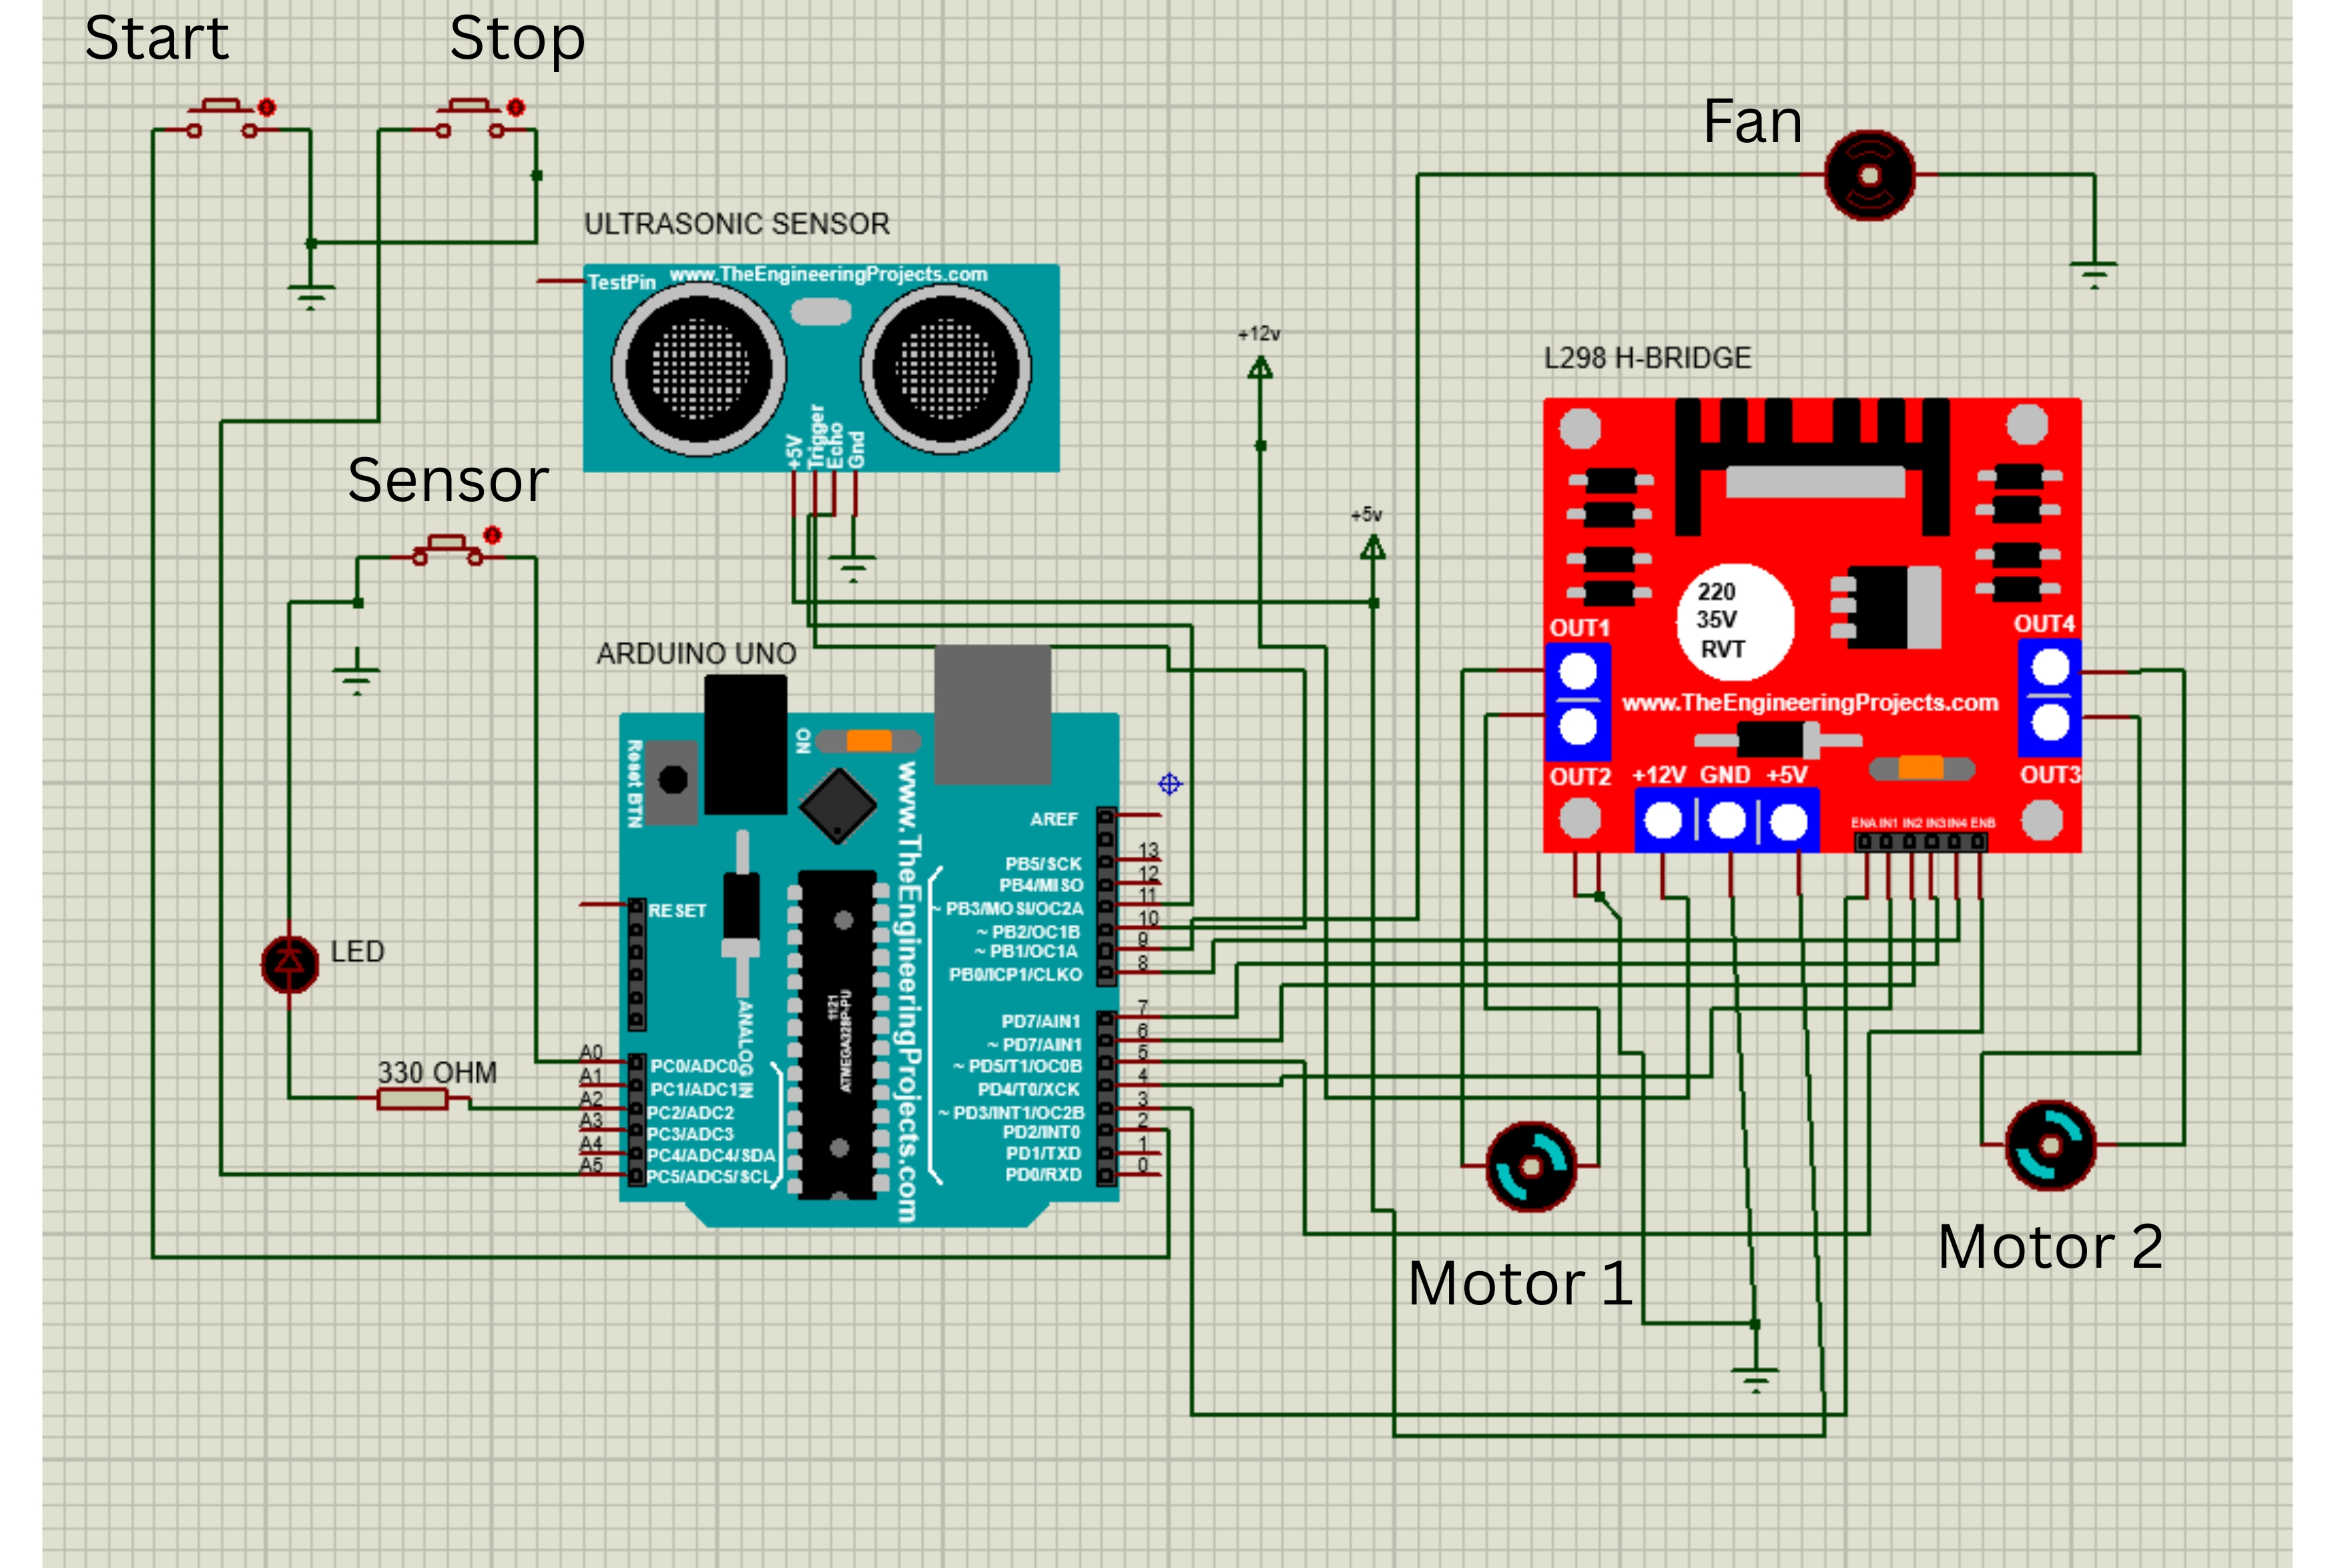
\includegraphics[width=\linewidth, keepaspectratio]{images/photos/proteus_simulation_shot.jpg}
        \caption{Proteus simulation of basic obstacle avoidance logic.}
        \label{fig:proteus_simulation_sub}
    \end{subfigure}
    \hfill % For spacing between subfigures
    \begin{subfigure}[b]{0.496\textwidth}
        \centering
        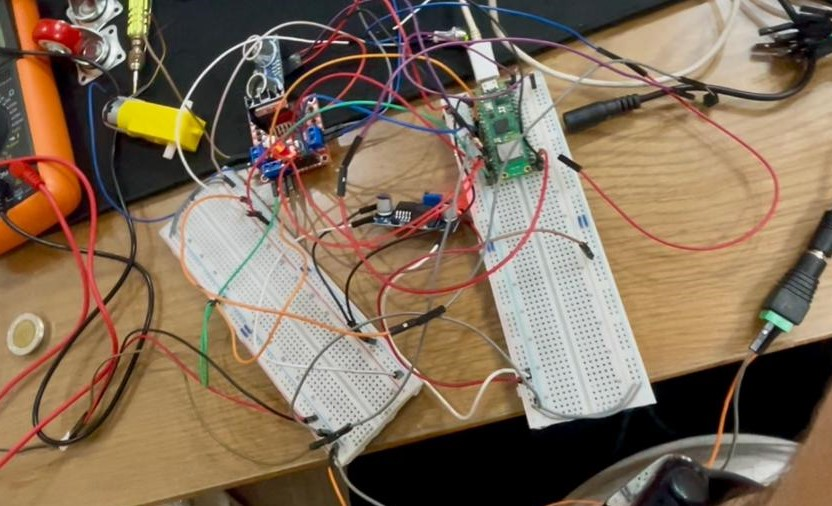
\includegraphics[width=\linewidth, keepaspectratio]{images/photos/breadboard_proto_shot.jpg}
        \caption{Breadboard prototype for physical validation.}
        \label{fig:breadboard_prototype_sub}
    \end{subfigure}
    \caption{Conceptual validation stages: (a) Proteus simulation of the robot's basic obstacle avoidance logic using an Arduino model, and (b) photograph of the breadboard prototype showing key component interconnections for physical validation.}
    \label{fig:combined_sim_breadboard}
\end{figure}

With the mechanical structure assembled, final electrical connections were made. Appropriate gauge wires were used for signal and power lines. Connections were double-checked for polarity and correctness against the wiring diagrams. Wire management involved routing cables to prevent interference with moving parts. Figure~\ref{fig:internal_wiring_photo_eval_new} shows the internal wiring with the custom \hyperref[term:pcb]{PCB}.
\begin{figure}[htbp]
    \centering
    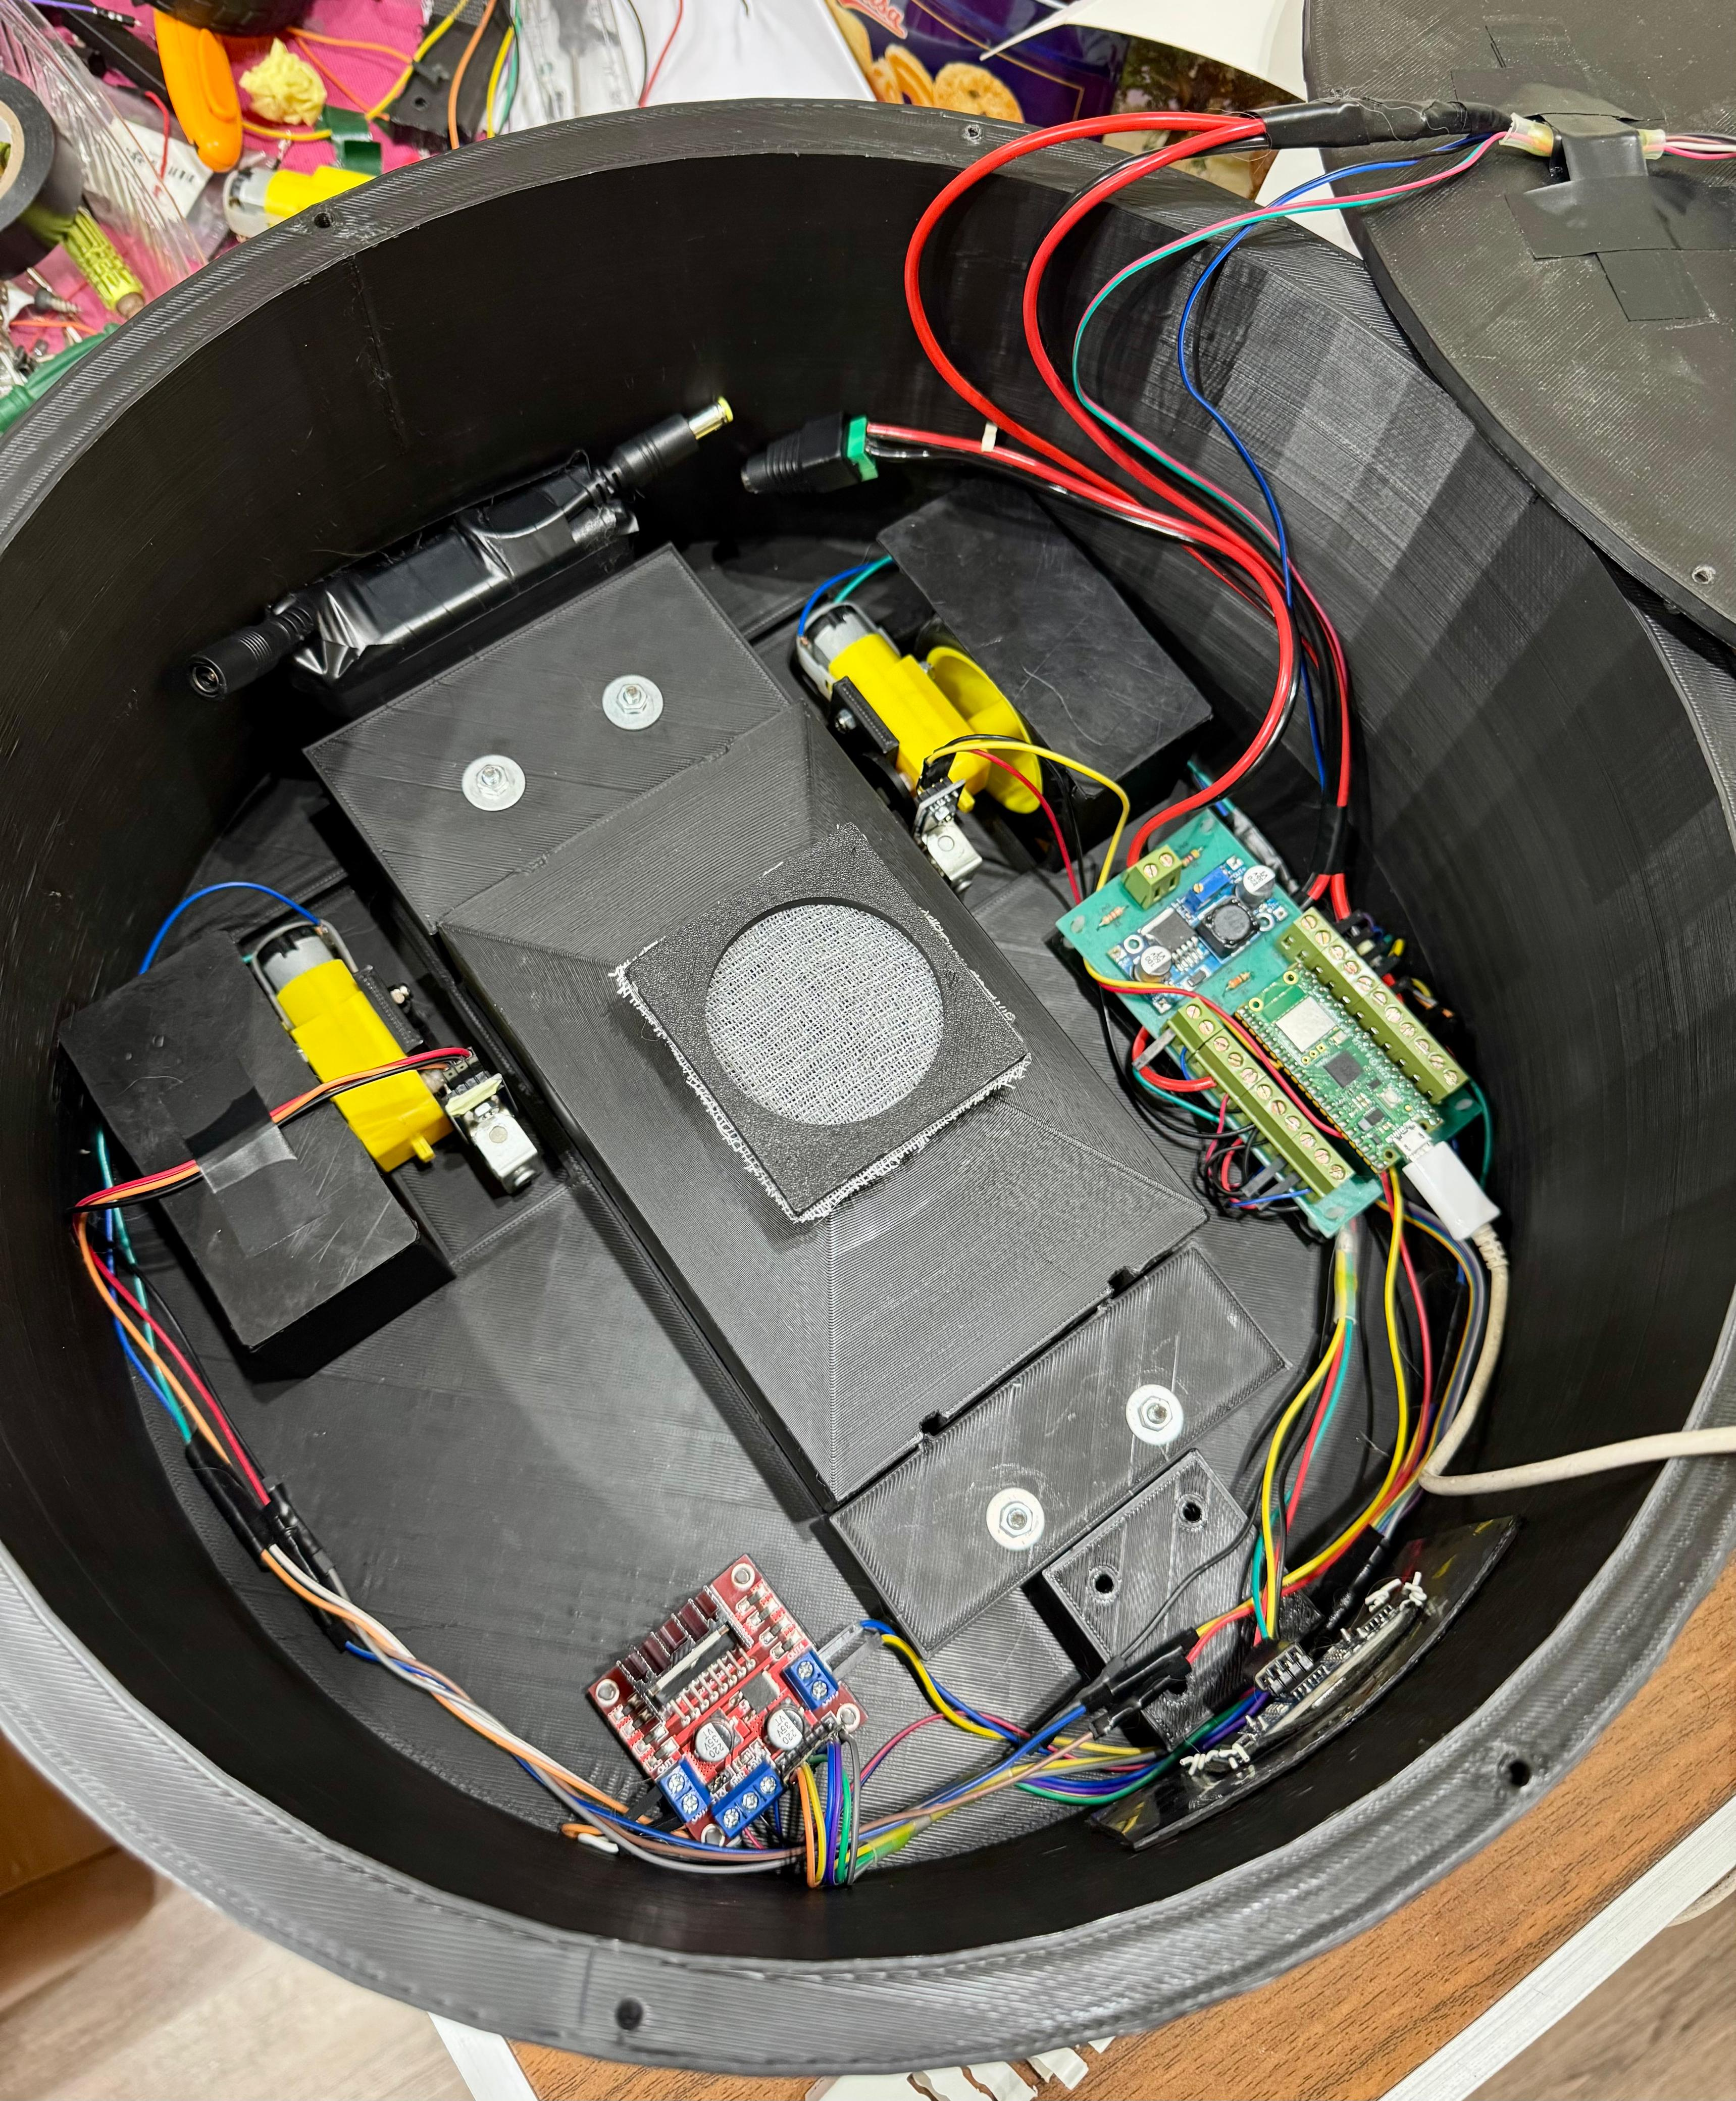
\includegraphics[width=\textwidth, keepaspectratio]{images/photos/internal_wiring.jpg}
    \caption{Internal view of the assembled robot showing component wiring and integration with the custom PCB.}
    \label{fig:internal_wiring_photo_eval_new} % Relabelled from fig:internal_wiring_photo_eval
\end{figure}


\subsection{Custom PCB Design and Fabrication}
\label{subsec:custom_pcb_design_new}
A custom 2-layer \hyperref[term:pcb]{PCB} (100mm x 50mm, FR4, 1oz copper, green solder mask, black legend) was designed in KiCad to integrate the Raspberry Pi Pico W, the LM2596S buck converter, screw terminals for external connections (motors, fan, sensor, button, \hyperref[term:led]{LED}), and the \hyperref[term:hcsr04]{HC-SR04} voltage divider circuit. This provided a more robust and organized solution than breadboard or perfboard wiring for the final prototype. The custom \hyperref[term:pcb]{PCB} served as the central point for connections, utilizing screw terminals for robust wiring to off-board components. The schematic, layout, and a 3D render of the \hyperref[term:pcb]{PCB} are shown in Figures \ref{fig:kicad_schematic_ctrl_new}, \ref{fig:kicad_layout_ctrl_new}, and \ref{fig:kicad_3d_render_ctrl_new} respectively.

It is important to note that the wheel encoders were integrated into the design as a post-manufacturing upgrade to enhance the robot's capabilities. Consequently, their wiring was connected directly to the Raspberry Pi Pico W's GPIO pins and is not reflected in the PCB schematic or layout diagrams (Figures \ref{fig:kicad_schematic_ctrl_new}, \ref{fig:kicad_layout_ctrl_new}).
\begin{figure}[htbp]
    \centering
    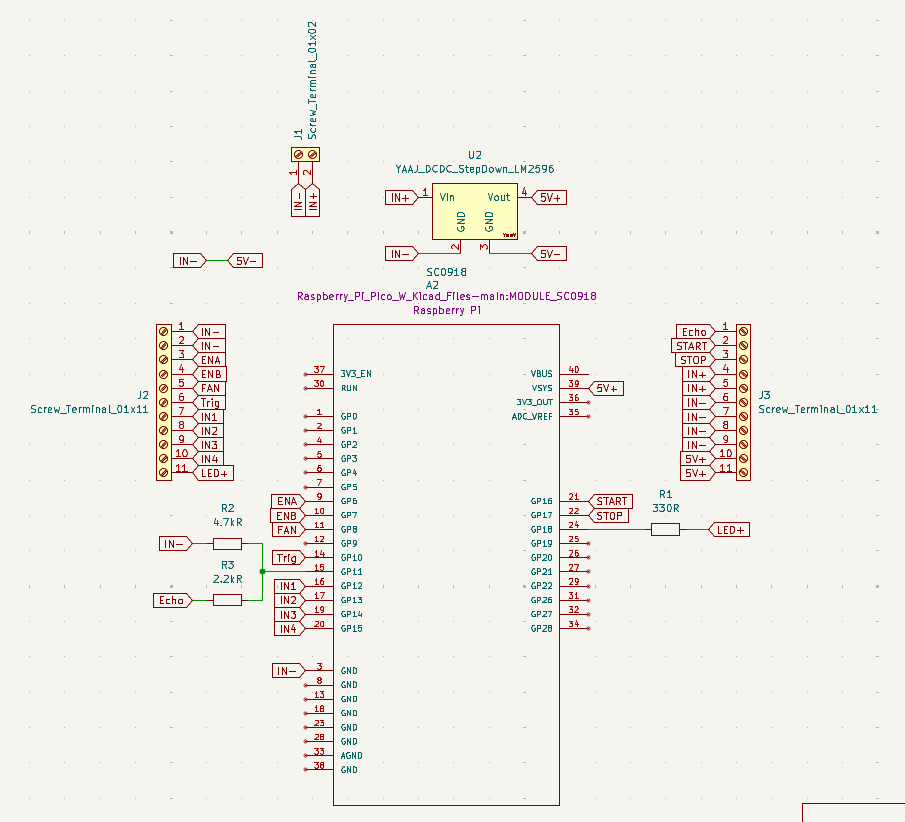
\includegraphics[width=\textwidth, keepaspectratio]{images/screenshots/kicad_schematic.png}
    \caption{KiCad schematic diagram for the custom Printed Circuit Board.}
    \label{fig:kicad_schematic_ctrl_new} % Relabelled from fig:kicad_schematic_ctrl
\end{figure}

\begin{figure}[htbp]
    \centering
    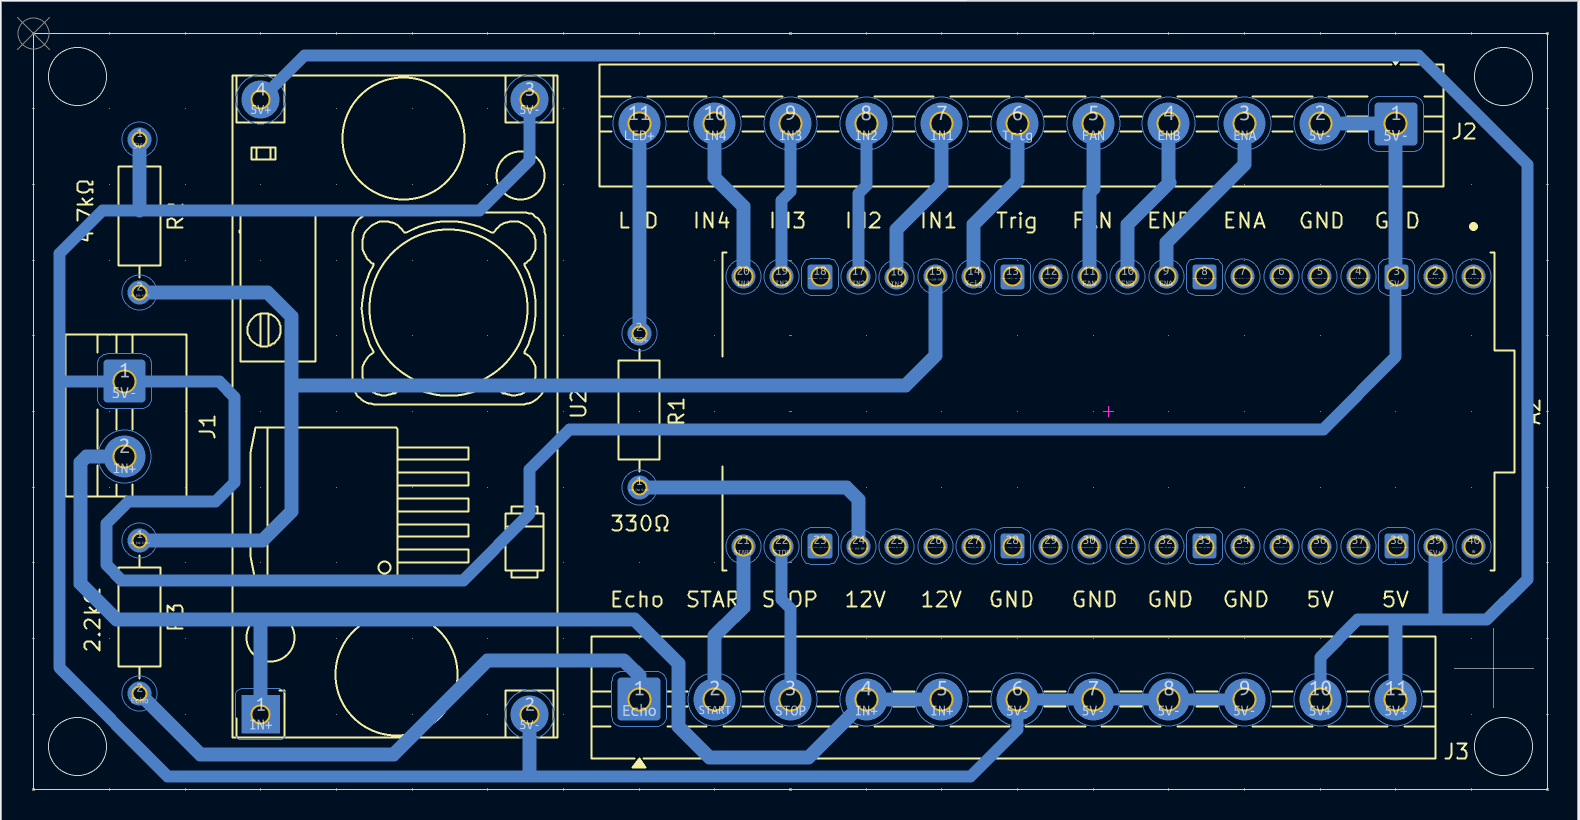
\includegraphics[width=0.928\textwidth, keepaspectratio]{images/screenshots/kicad_layout.png}
    \caption{KiCad PCB layout design (2D view).}
    \label{fig:kicad_layout_ctrl_new} % Relabelled from fig:kicad_layout_ctrl
\end{figure}

\begin{figure}[htbp]
    \centering
    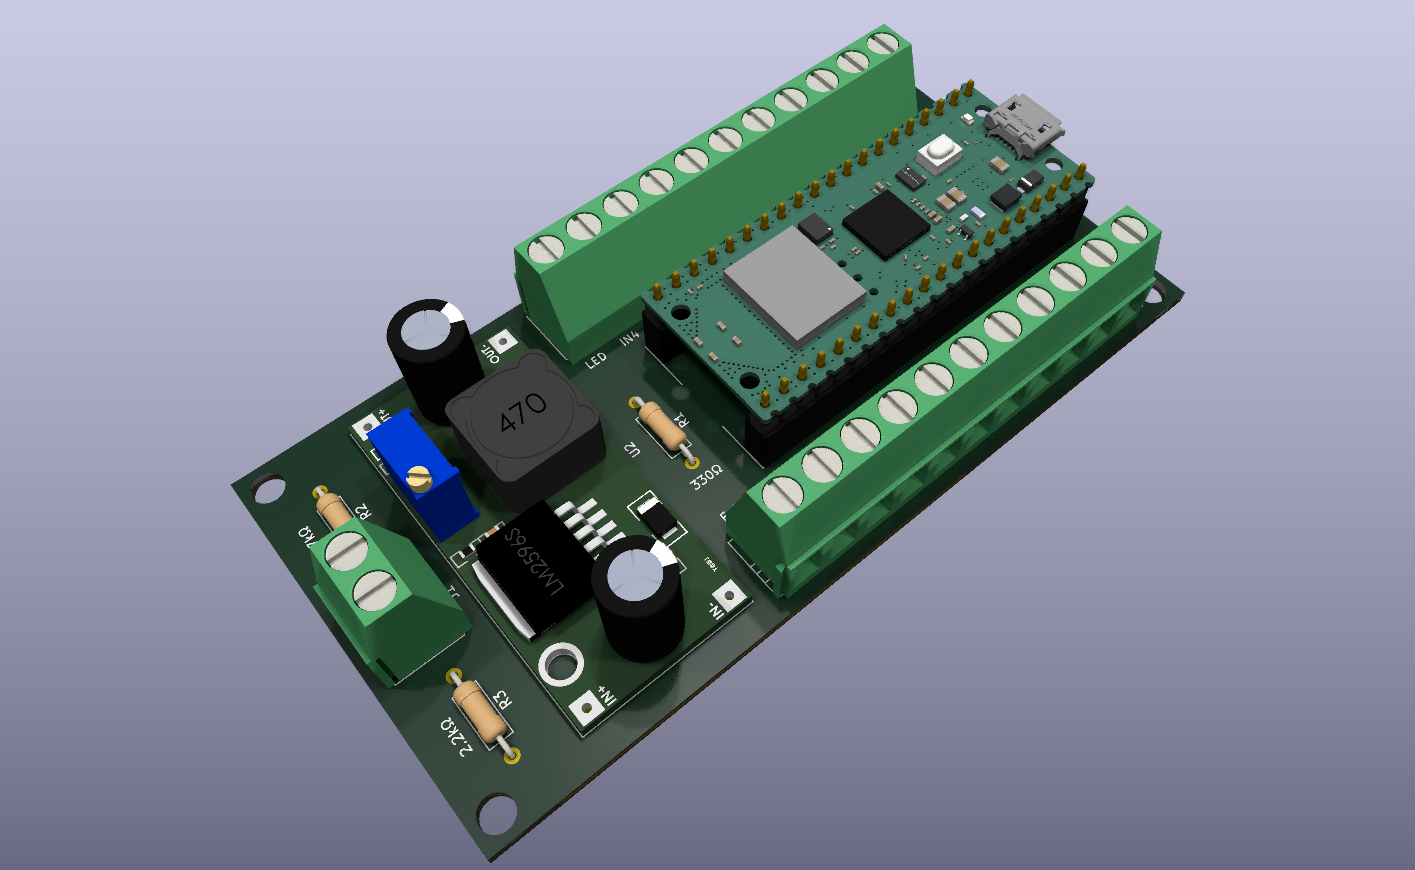
\includegraphics[width=0.928\textwidth, keepaspectratio]{images/screenshots/kicad_3d_render.png}
    \caption{3D rendering of the populated PCB design from KiCad.}
    \label{fig:kicad_3d_render_ctrl_new} % Relabelled from fig:kicad_3d_render_ctrl
\end{figure}

\section{Control System Implementation (Software)}
\label{sec:control_implementation_software_ctrl_new} % Relabelled from old sec:control_implementation_software_ctrl
The robot's behavior is governed by software developed in MicroPython, running on the Raspberry Pi Pico W. The complete source code is provided as an accompanying file (\texttt{code\_backup/main.py}).
\subsection{Software Architecture}
\label{subsec:software_architecture_new}
The software is structured modularly to handle various tasks:
\begin{itemize}
    \item \textbf{Hardware Abstraction Layer}: Functions to initialize and interact with hardware peripherals, including hardware interrupt handlers for the wheel encoders.
    \item \textbf{\hyperref[term:pid]{PID} Control Module}: Contains the feed-forward PWM calculation (\texttt{ff\_pwm}), straight-line motion with positional PID (\texttt{straight\_motion}), and pivot turns with a dual progress/balance PID (\texttt{pivot\_motion}).
    \item \textbf{Autonomous State Machine}: Implements the primary logic for autonomous cleaning as a finite state machine: \texttt{IDLE} $\to$ \texttt{START\_FWD} $\to$ \texttt{FWD} (moving forward until an obstacle is detected) $\to$ \texttt{START\_AVOID} $\to$ \texttt{AVOID} (executing a wide turn), with a \texttt{STALL\_TURN} recovery state triggered by motor stall detection.
    \item \textbf{Safety and Monitoring Layer}: Includes critical functions for motor stall detection, active braking, and an emergency stop protocol to ensure safe operation.
    \item \textbf{User Interface Module}: Manages inputs from the physical start/stop button and the \hyperref[term:ble]{BLE} remote, and controls the status \hyperref[term:led]{LED}.
    \item \textbf{Main Control Loop}: Uses a priority-based execution model---first handling horn/obstacle blocking, then manual commands with toggle behavior, then the autonomous finite state machine---while continuously updating the LED feedback system.
\end{itemize}

\begin{figure}[htbp]
    \centering
    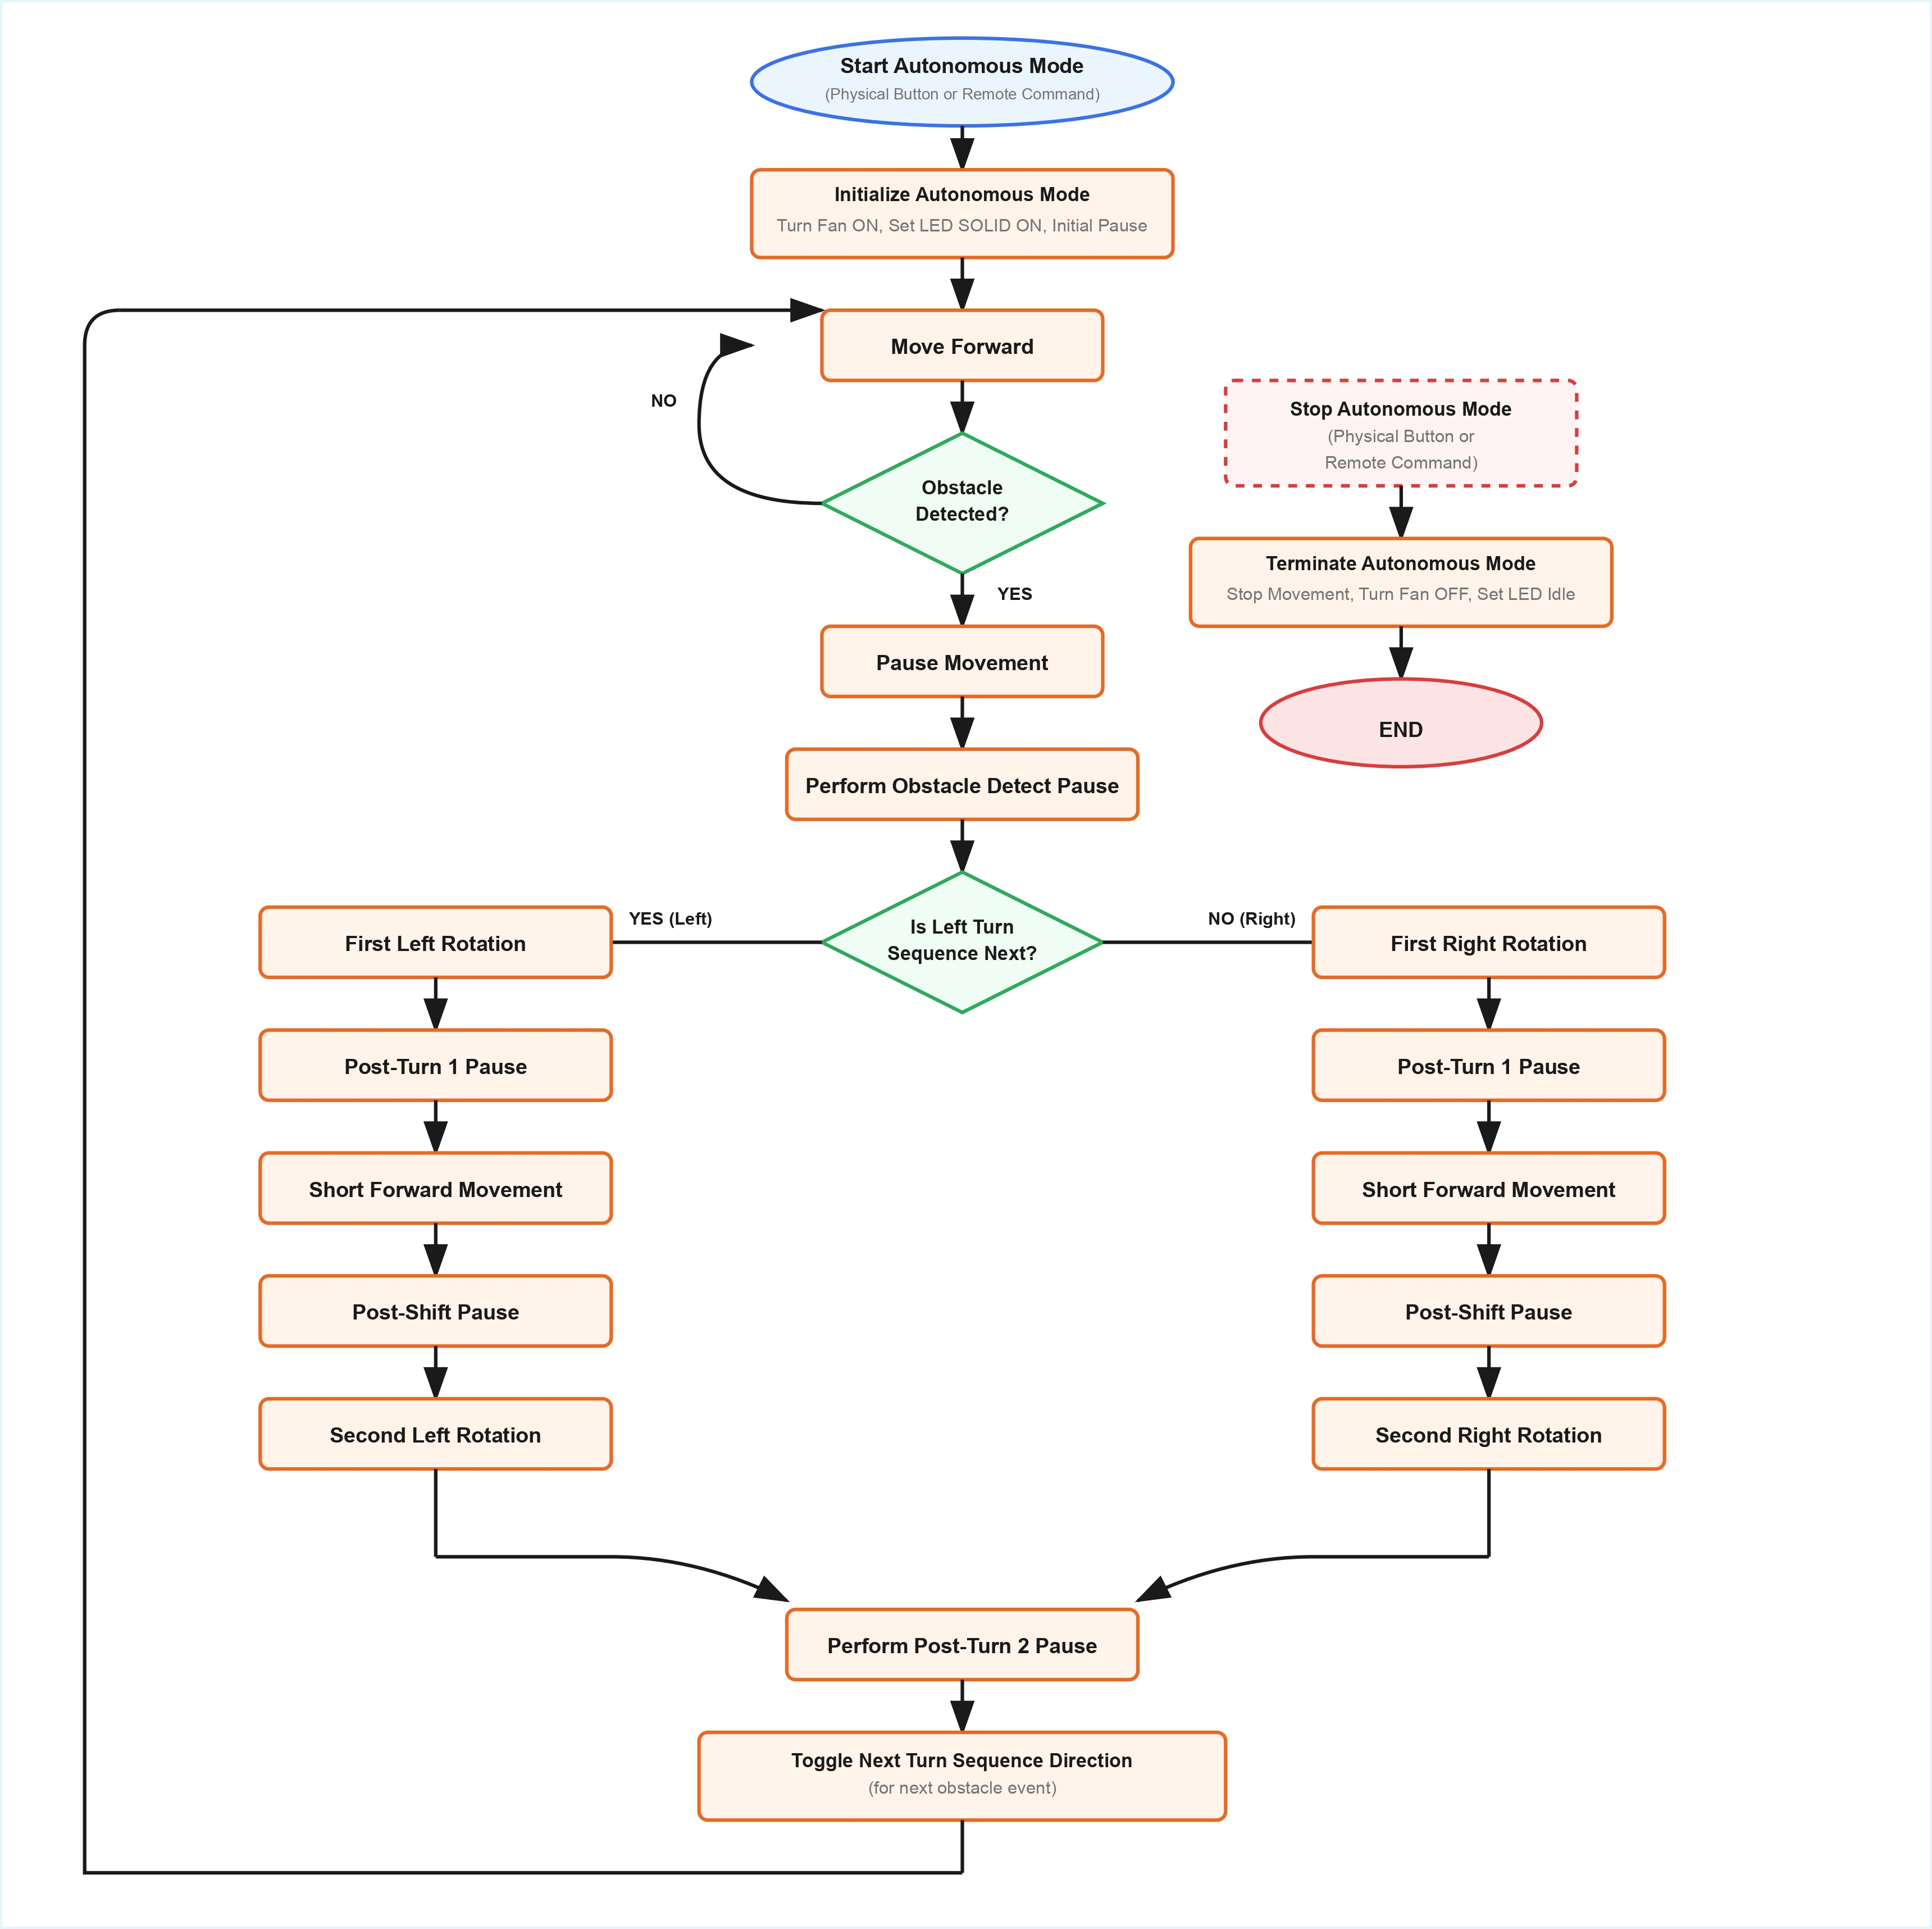
\includegraphics[width=0.85\textwidth]{images/screenshots/software_flowchart.jpg}
    \caption{Block diagram of the autonomous obstacle-avoidance state machine showing the robot's operational states and transitions.}
    \label{fig:flowchart_autonomous_logic_ctrl_new}
\end{figure}


\subsection{Evolution of the Control Strategy}
\label{subsec:control_strategy_evolution}
The initial navigation strategy was purely reactive and time-based, which lacked precision. The introduction of wheel encoders enabled a more sophisticated, closed-loop system. The development evolved from a pure feedback approach to a more robust hybrid model.

\subsubsection{Limitation of Pure \texorpdfstring{\hyperref[term:pid]{PID}}{PID} Control}
The first closed-loop attempts used a \textbf{Positional \hyperref[term:pid]{PID}} controller. This controller's error term was calculated from the difference in the total distance traveled by each wheel (\texttt{left\_pulses - right\_pulses}) to actively correct for drift. While a significant improvement, this purely reactive system was susceptible to a critical hardware limitation: aggressive \hyperref[term:pid]{PID} adjustments, especially during turns, would attempt to draw excessive current to compensate for motor differences. This led to voltage sags (\textbf{brownouts}) that would stall a motor, causing the control system to fail catastrophically. This discovery highlighted that a superior software algorithm can be defeated by the physical limitations of its hardware.

\subsubsection{Final Implemented Architecture: Hybrid Feed-Forward and \texorpdfstring{\hyperref[term:pid]{PID}}{PID} Control}
To create a more robust system, a \textbf{hybrid feed-forward and feedback} architecture was developed, as reflected in the accompanying source code (\texttt{main.py}).
\begin{itemize}
    \item \textbf{Feed-Forward (FF) Model}: A simple linear model (\texttt{ff\_pwm}) was created to proactively estimate the required \hyperref[term:pwm]{PWM} signal for a given target speed (in pulses per second). This forms the primary, anticipatory part of the controller, providing the ``muscle'' for a given movement based on the desired outcome.
    \item \textbf{\hyperref[term:pid]{PID} as a Correction Layer}: The positional \hyperref[term:pid]{PID} controller was retained but repurposed. Instead of calculating the entire motor command, it now calculates a small \textit{adjustment} to the target speed. This feedback layer acts as a fine-tuner, correcting for small, unmodeled errors (e.g., wheel slip, friction changes) without making the large, aggressive power demands that previously caused system instability.
    \item \textbf{Manual Control Enhancement}: The manual control logic was updated to a toggle system. Sending a movement command (e.g., ``FORWARD'') initiates the motion; sending the same command a second time applies the brake and stops the robot, providing more intuitive control.
    \item \textbf{Stall Detection and Recovery}: A safety-critical routine was integrated. During autonomous movement, the software checks if the encoder pulses have stopped. If the robot is physically stuck, it triggers a recovery state where it reverses and turns to free itself.
\end{itemize}
This journey from a simple reactive system to a hardware-aware hybrid controller demonstrates a comprehensive engineering process of design, testing, diagnosis, and refinement.

\subsubsection{PID Tuning Methodology}
\label{subsubsec:pid_tuning}
The \hyperref[term:pid]{PID} gains ($K_p$, $K_i$, $K_d$) were determined through an empirical trial-and-error process, a practical approach suitable for this prototype. The tuning followed a systematic procedure:
\begin{enumerate}
    \item \textbf{Start with P only}: Initially, only proportional gain was applied. The value was increased until oscillation occurred, then reduced.
    \item \textbf{Add D for damping}: Derivative gain was introduced to reduce overshoot and smooth the response.
    \item \textbf{Add minimal I}: A small integral term was added to eliminate steady-state drift, with careful limiting to prevent windup.
\end{enumerate}
The final tuned values for the positional correction \hyperref[term:pid]{PID} were conservative (low gains) to avoid the brownout conditions described earlier. This trade-off prioritized system stability over aggressive correction, accepting slightly less precise correction in exchange for reliable operation.

\subsection{\texorpdfstring{\hyperref[term:ble]{BLE}}{BLE} Remote Control}
\label{subsec:ble_remote_control_ctrl_new} % Relabelled from old subsec:ble_remote_control_ctrl
The Raspberry Pi Pico W's \hyperref[term:ble]{BLE} capability is utilized for manual remote control. A \hyperref[term:ble]{BLE} \hyperref[term:uart]{UART} service is implemented on the Pico W, allowing it to receive commands from a connected \hyperref[term:ble]{BLE} central device, typically a smartphone running a compatible application.
\subsubsection*{NRF Toolbox Application}
For this project, the NRF Toolbox application (or a similar \hyperref[term:ble]{BLE} \hyperref[term:uart]{UART} terminal app) can be used to interact with the robot. The application connects to the Pico W's \hyperref[term:ble]{BLE} service and allows the user to send text-based commands over the \hyperref[term:uart]{UART} profile.
\begin{itemize}
    \item \textbf{Connection}: The user scans for \hyperref[term:ble]{BLE} devices and connects to the robot, which advertises with a unique name (e.g., ``PicoRobot-3C33'').
    \item \textbf{Command Interface}: The \hyperref[term:uart]{UART} interface in the NRF Toolbox app provides a console or programmable buttons to send specific string commands to the robot. The MicroPython code on the Pico W (\texttt{main.py}) is programmed to recognize commands such as ``FORWARD'', ``BACKWARD'', ``LEFT'', ``RIGHT'', ``CLEAN'', ``FAN'', and ``HORN''. A key feature of manual control is that sending the same movement command twice acts as a toggle, stopping the robot.
    \item \textbf{Functionality}: This setup enables direct manual control of the robot's movements and functions, providing an alternative to the autonomous mode and facilitating testing or direct intervention.
\end{itemize}
Figure~\ref{fig:nrf_toolbox_ui_new} shows an example user interface. The integration of \hyperref[term:ble]{BLE} significantly enhances the robot's usability and interactivity.

\subsubsection*{Safety Feature - Manual Obstacle Block}
The system implements a safety feature for manual forward movement. If the user commands the robot forward but the ultrasonic sensor detects an obstacle, the software flags the robot as blocked. It stops the motors and activates a buzzing sound to alert the user, preventing a collision. The user must then command a different direction (e.g., backward or turn) to clear the flag.


\begin{figure}[htbp]
    \centering
    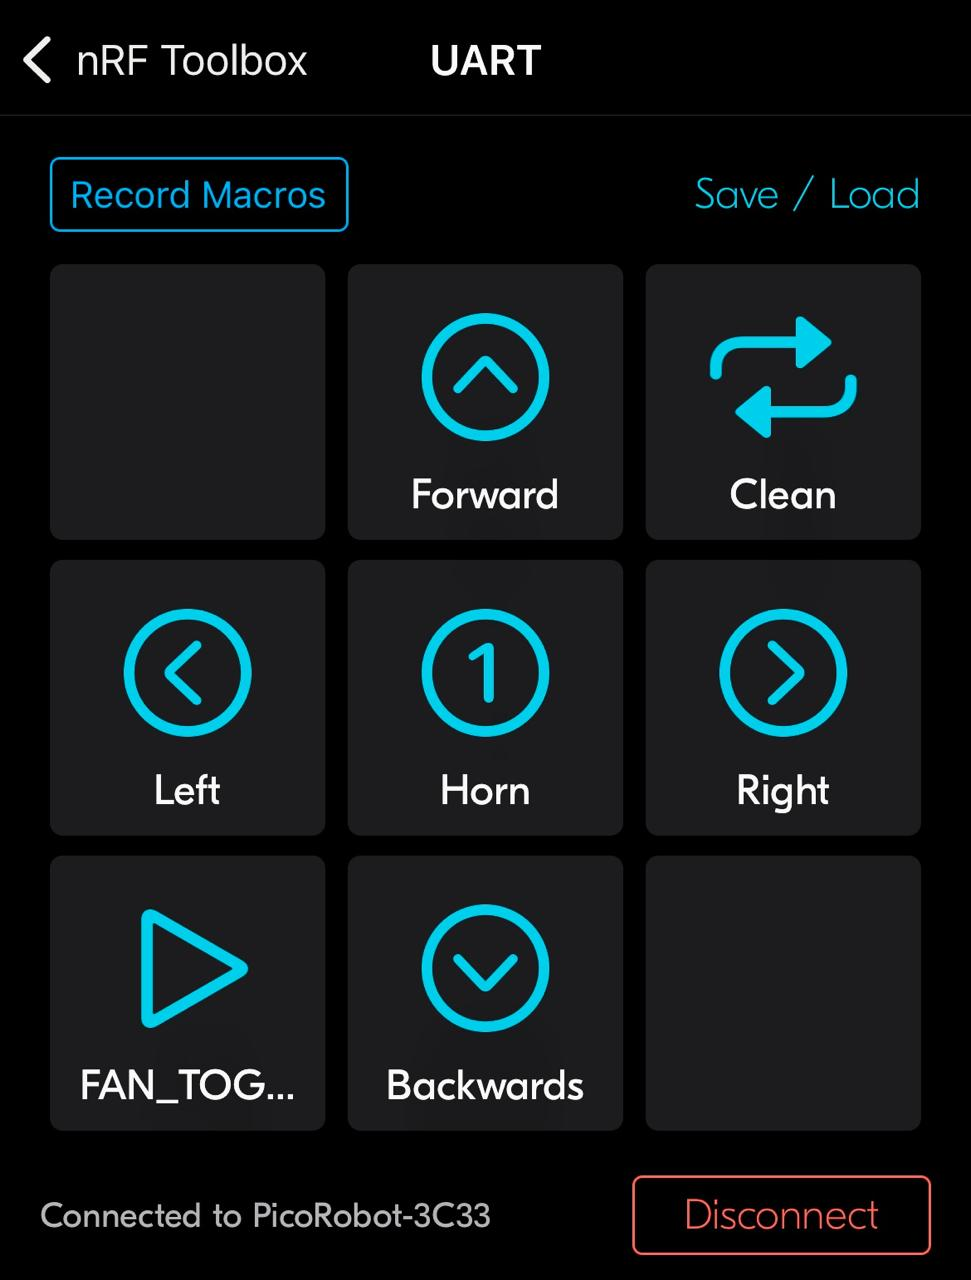
\includegraphics[width=0.401\textwidth, keepaspectratio]{images/screenshots/nrf_toolbox_ui.jpg}
    \caption{Example user interface of the NRF Toolbox application configured for controlling the Smart Cleaning Robot via BLE UART.}
    \label{fig:nrf_toolbox_ui_new} % Relabelled from fig:nrf_toolbox_ui
\end{figure}

\subsection{Software Deployment}
\label{subsec:software_deployment_new}
The MicroPython firmware was flashed onto the Raspberry Pi Pico W. The control script (\texttt{main.py}) was uploaded using the Thonny \hyperref[term:ide]{IDE}, as shown in Figure~\ref{fig:thonny_ide_screenshot_eval_new}. A \texttt{boot.py} script was configured to enable WebREPL for wireless debugging and parameter tuning during development.
\begin{figure}[htbp]
    \centering
    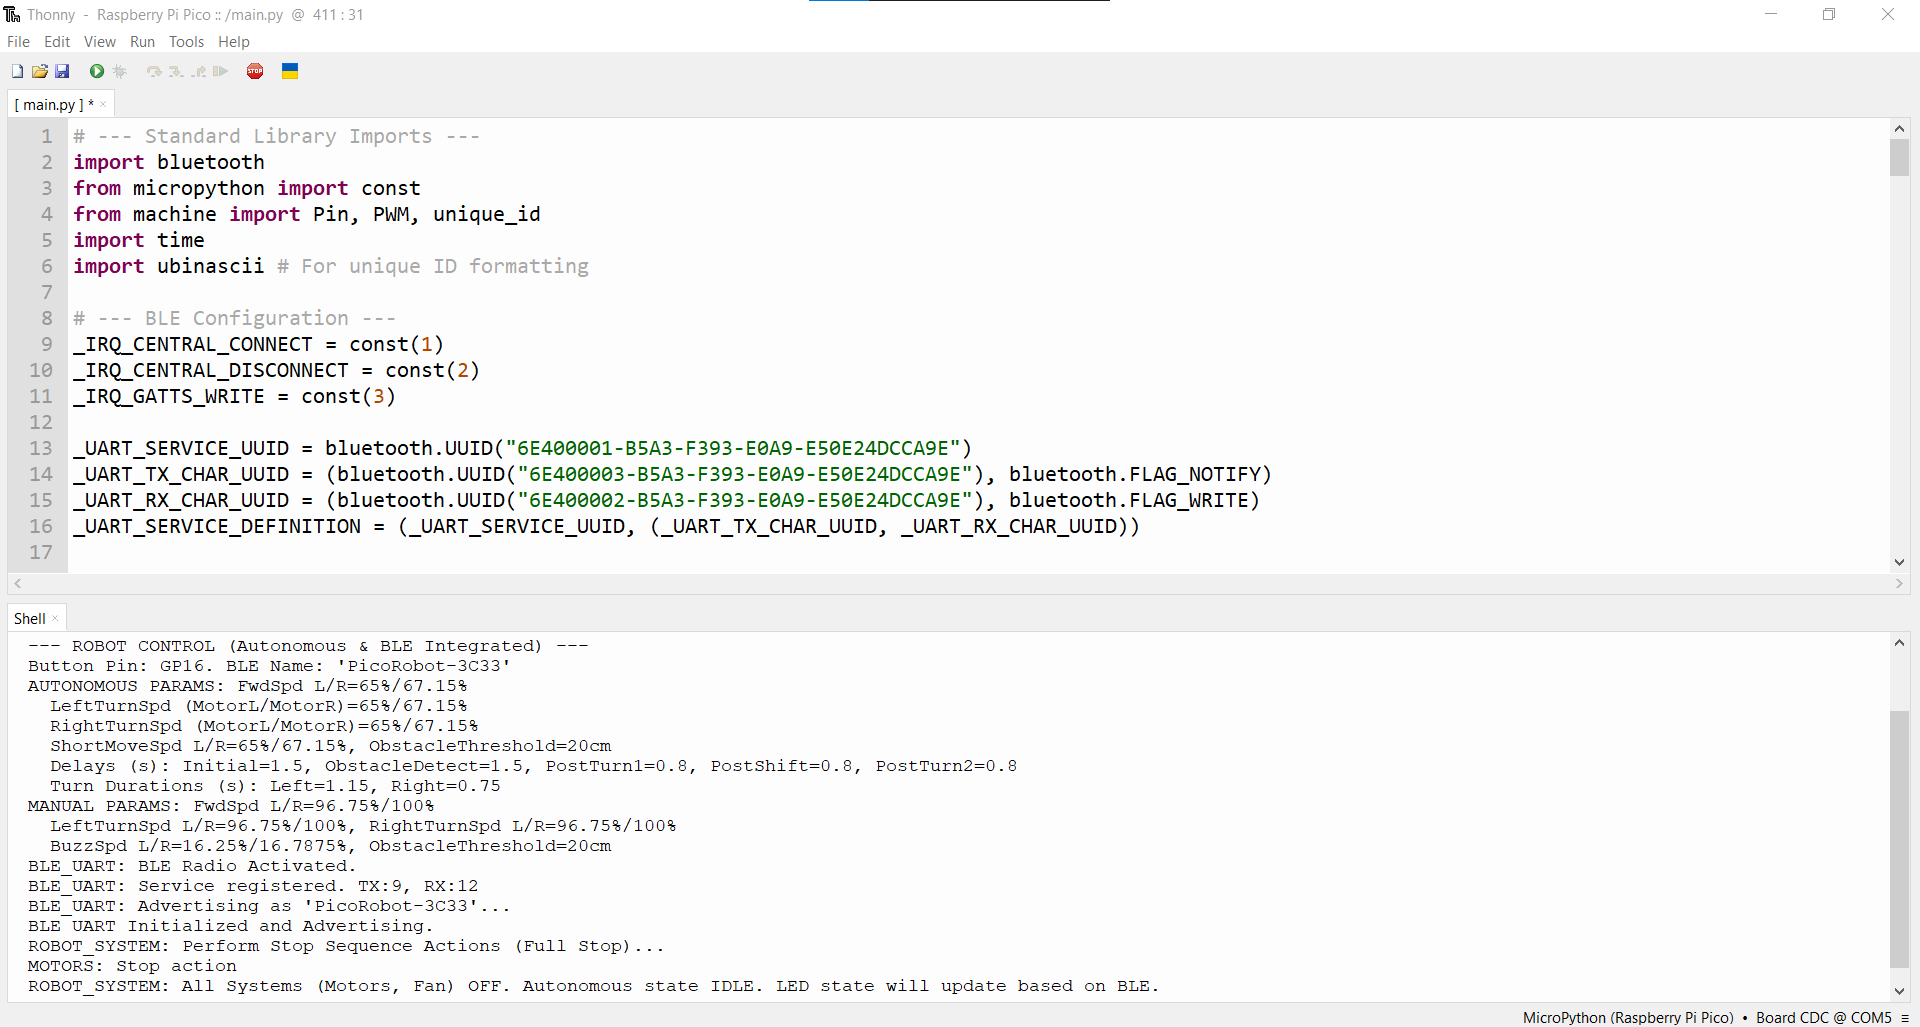
\includegraphics[width=0.85\textwidth, keepaspectratio]{images/screenshots/thonny_ide.png}
    \caption{Screenshot of Thonny IDE showing the MicroPython control script deployed to the Raspberry Pi Pico W.}
    \label{fig:thonny_ide_screenshot_eval_new} % Relabelled from fig:thonny_ide_screenshot_eval
\end{figure}


\section{Performance Evaluation and Results}
\label{sec:performance_evaluation_eval_new}

The evaluation focused on functional verification of core features and qualitative observation of the robot's behavior in a typical indoor test environment.
\subsection{Functional Verification and Observations}
\label{subsec:functional_verification_observations_new}

\begin{itemize}
    \item \textbf{Manual \hyperref[term:ble]{BLE} Remote Control}: Functioned perfectly. The robot exhibited prompt and accurate responses to commands sent via the NRF Toolbox application, with good connection stability over several meters. The \hyperref[term:pid]{PID}-assisted forward command was noticeably straighter than unassisted control.
    \item \textbf{Autonomous Navigation}: The integration of wheel encoders and a \hyperref[term:pid]{PID} control system resulted in a significant improvement in navigational accuracy over the previous open-loop system. Straight-line movement was noticeably more stable, with the positional \hyperref[term:pid]{PID} controller effectively mitigating much of the drift caused by motor and surface inconsistencies. While not perfectly precise in all scenarios, the robot could now execute its back-and-forth cleaning pattern more reliably. The dual-objective \hyperref[term:pid]{PID} controller produced more consistent turn angles. Furthermore, the newly implemented stall detection and recovery feature was tested and found to be effective in simulated ``stuck'' conditions.
    \item \textbf{Vacuum System Performance}:
        \begin{itemize}
            \item \textit{Debris Collection:} The vacuum system, using the PS3 fan, collected light debris like small paper pieces and dust from hard floor surfaces.
            \item \textit{Limitations:} Performance was constrained by two main factors: the absence of a check valve, leading to occasional spillage of collected debris at the end of an operation, and the unavailability of brushes, which limited the robot's ability to dislodge embedded dirt.
        \end{itemize}
    \item \textbf{Power System}: The 12V \hyperref[term:liion]{Li-ion} battery pack~\cite{BatteryPack12V4000mAhDatasheet} and LM2596S buck converter provided stable power, achieving an operational runtime exceeding 60 minutes on a full charge during continuous autonomous operation. The overall system current and power are approximately \totalCurrent{} and \totalPower{} respectively, at a nominal \totalVoltage{}. This estimate is based on the main power-consuming components: the PS3 fan (rated $\sim$1.3A at 12V), and the two DC motors, which can draw over 0.8A combined under operational load. The remaining electronics contribute a smaller fraction to the total consumption. Peak current during motor startup or simultaneous operation of all high-draw components could be higher.
    \item \textbf{User Interface (Button/\hyperref[term:led]{LED})}: The physical start/stop button and status \hyperref[term:led]{LED} functioned as designed, providing correct user interaction and feedback.
\end{itemize}

Table~\ref{tab:test_results} summarizes the key performance metrics observed during testing.

\begin{table}[htbp]
\centering
\caption{Performance Test Results Summary.}
\label{tab:test_results}
\begin{tabular}{|l|c|l|}
\hline
\textbf{Metric} & \textbf{Result} & \textbf{Notes} \\ \hline
BLE Connection Range & $>$5 m & Stable indoor connection \\ \hline
Straight-Line Stability & Good & PID reduces drift significantly \\ \hline
Turn Angle Consistency & Improved & More reliable than open-loop \\ \hline
Stall Detection & Functional & Recovery sequence works \\ \hline
Battery Runtime & $>$60 min & Continuous operation \\ \hline
Debris Collection & Light debris & Paper, dust on hard floors \\ \hline
System Power & $\sim$26W & At \totalVoltage{} nominal \\ \hline
\end{tabular}
\end{table}
\subsection{Summary}
\label{subsec:discussion_performance_evaluation_new}

The performance evaluation indicates that the upgrade to a closed-loop, \hyperref[term:pid]{PID}-based control system was a success. While not achieving perfect motion, it dramatically improved the precision and reliability of the robot's movement compared to the initial prototype. The implemented control system enabled the robot's autonomous behavior to be more systematic and, crucially, allowed for the integration of vital safety features like stall detection and recovery. The custom \hyperref[term:pcb]{PCB} and overall physical construction represent a solid prototyping effort.

The evaluation also confirms that achieving flawless path execution with the current DC motor and chassis setup remains a challenge. The vacuum system, while functional for light debris, also has clear limitations impacting its practical cleaning effectiveness. These findings are valuable insights that directly inform the recommendations for future work.

% --- NEW Chapter 5: Conclusion and Recommendations for Future Work ---
\chapter{Conclusion and Recommendations for Future Work}
\label{chap:conclusion_future_work_new}

\section{Conclusion}
\label{sec:conclusion_summary_new}
This thesis has successfully detailed the design, implementation, and qualitative performance evaluation of a prototype Smart Cleaning Robot. The project was undertaken with the aim of developing a cost-effective automated cleaning solution, leveraging the Raspberry Pi Pico W microcontroller, readily available sensors, and custom 3D-printed components.
Key achievements of this project include:
\begin{itemize}
    \item The development of a functional robot prototype capable of \hyperref[term:ble]{BLE}-based manual remote control, featuring an autonomous navigation system upgraded to a hardware-aware, hybrid feed-forward and \hyperref[term:pid]{PID} control strategy.
    \item A comprehensive design process encompassing mechanical design using SolidWorks, electrical system design with a custom \hyperref[term:pcb]{PCB}, and an iterative embedded software development process in MicroPython that explored multiple control theories.
    \item Successful integration of various hardware components, including the Raspberry Pi Pico W, \hyperref[term:hcsr04]{HC-SR04} ultrasonic sensor, \hyperref[term:l298n]{L298N} motor driver, wheel encoders, and a repurposed PS3 fan for the vacuum system.
    \item The implementation of a robust physical prototype with a neatly assembled chassis and electronics, capable of demonstrating significantly improved, though not perfect, autonomous movement.
    \item Functional verification showing excellent remote-control capabilities, a basic ability to collect light debris, and the successful operation of safety features like stall detection.
\end{itemize}

\subsection{Cost Analysis}
\label{subsec:cost_analysis}
A primary objective of this thesis was to demonstrate the feasibility of a cost-effective cleaning robot. Table~\ref{tab:cost_comparison} compares the prototype's total cost against representative commercial alternatives.

\begin{table}[htbp]
\centering
\caption{Cost Comparison: Prototype vs. Commercial Robots.}
\label{tab:cost_comparison}
\begin{tabular}{|l|c|c|}
\hline
\textbf{Robot} & \textbf{Approx. Cost (USD)} & \textbf{Key Features} \\ \hline
This Prototype & \$80 (3950 EGP) & BLE control, PID nav, vacuum \\ \hline
Basic Robot Vacuums & \$100--200 & Random nav, basic vacuum \\ \hline
Xiaomi X20 Plus & \$300--500 & LiDAR SLAM, auto-empty \\ \hline
iRobot Roomba 980 & \$500--900 & vSLAM, smart features \\ \hline
\end{tabular}
\end{table}

The prototype achieves its core functionality at approximately \textbf{60--90\% lower cost} than entry-level commercial robots. While it lacks advanced features like SLAM-based navigation, it provides a functional platform demonstrating that affordable home robotics is achievable with accessible components.
Ultimately, this project effectively demonstrated the feasibility of creating a smart cleaning robot with a modest budget and accessible technology. The iterative design process, especially in refining the software control strategy, was crucial for overcoming hardware challenges and achieving a higher level of functionality. The resulting prototype serves as a valuable foundation for affordable home robotics, successfully balancing core functionality with cost-effectiveness and providing a clear pathway for the more sophisticated enhancements outlined in this chapter.

\section{Limitations}
\label{sec:limitations_conclusion_new}
Despite the progress made, the current prototype and project have several limitations that should be acknowledged:
\begin{itemize}
    \item \textbf{Autonomous Navigation Precision}: While the implementation of wheel encoders and \hyperref[term:pid]{PID} control represents a major advancement, achieving perfect navigational precision remains a primary limitation. Inherent non-linearities in the low-cost DC gear motors result in small, cumulative errors. This issue is compounded by the fact that the wheel encoders were integrated after the initial chassis was fabricated, leading to mounting points that are not perfectly symmetrical and contributing to small, cumulative errors. The \hyperref[term:pid]{PID} system works to actively correct these errors, but it cannot eliminate them entirely.
    \item \textbf{Lack of High-Level Path Planning}: The current system uses its enhanced precision to better execute its reactive coverage strategy (moving forward and turning at obstacles or after recovering from stalls). However, it lacks advanced mapping and localization capabilities, such as those enabled by \hyperref[term:slam]{SLAM} techniques. This absence restricts the robot to reactive strategies rather than enabling truly intelligent, map-based environmental coverage, such as the systematic Boustrophedon pattern discussed in Chapter 2.
    \item \textbf{Vacuum System Effectiveness}:
        \begin{itemize}
            \item \textit{No Check Valve:} The absence of a check valve in the Debris Collection Chamber can cause collected debris to spill out when the fan is turned off or the robot is jostled.
            \item \textit{No Brushes:} The lack of mechanical brushes (roller or side), due to the local unavailability of suitable off-the-shelf components, significantly reduces the robot's ability to dislodge dirt from carpets or effectively clean edges and corners.
        \end{itemize}
    \item \textbf{Basic Power Management}: The current system uses a battery and buck converter but lacks advanced power management features such as battery level monitoring, low-battery warnings, or automatic return-to-charge functionality.
\end{itemize}
\section{Lessons Learned}
\label{sec:lessons_learned}
The development of this prototype provided valuable engineering insights beyond the technical outcomes:
\begin{itemize}
    \item \textbf{Hardware-Software Interaction}: The brownout issue highlighted that software algorithms cannot compensate for hardware limitations. Understanding the electrical constraints of the system is essential before designing control strategies.
    \item \textbf{Iterative Design Value}: The evolution from open-loop to PID to hybrid control demonstrated the importance of iterative refinement. Each failure mode informed subsequent design decisions.
    \item \textbf{Component Sourcing Challenges}: Local unavailability of certain components (brushes, specific sensors) required creative alternatives. Future projects should include sourcing contingencies.
    \item \textbf{Early Encoder Integration}: Adding wheel encoders post-fabrication led to asymmetric mounting. Integrating precision sensors from the initial design phase would improve performance.
    \item \textbf{Documentation Throughout}: Maintaining detailed notes during debugging accelerated problem diagnosis and solution development.
\end{itemize}

\section{Recommendations for Future Work}
\label{sec:future_work_new}
The current prototype serves as a strong foundation for numerous potential enhancements and future research directions, directly addressing the identified limitations:
\begin{enumerate}
    \item \textbf{Improved Navigation and Sensing:}
        \begin{itemize}
            \item \textbf{Upgrade Drive Motors (Stepper or High-Torque DC):} To overcome the inherent precision limitations of the current DC motors, future work should investigate replacing them with alternatives like stepper motors. Steppers offer open-loop control with a high degree of accuracy, which could eliminate path deviation issues. Furthermore, selecting motors with higher torque—whether they are steppers or simply more robust DC gear motors—is crucial. This would improve performance on thicker carpets and enhance the robot's capability to overcome small obstacles.
            \item \textbf{Refined Path Planning Logic}: The successful integration of wheel encoders provides reliable odometry, paving the way for more intelligent navigation. Future work could leverage this improved positional awareness to implement more systematic algorithms, such as a true wall-following routine for thorough edge and corner cleaning, which would be a logical next step beyond the current obstacle-avoidance pattern.
            \item \textbf{Explore \hyperref[term:slam]{SLAM}}: As a more advanced step, consider upgrading the processing capabilities (e.g., to a Raspberry Pi 4 with \hyperref[term:ros]{ROS}) to integrate a \textbf{\hyperref[term:lidar]{LiDAR}} sensor for 360-degree environmental mapping. This would allow the robot to build a precise 2D map and enable truly intelligent navigation, moving beyond simple obstacle avoidance to strategic, map-based cleaning, which would enable the implementation of efficient coverage algorithms like the Boustrophedon pattern~\cite{DurrantWhyte2006SLAM}.
        \end{itemize}
    \item \textbf{Enhanced Cleaning Mechanism:}
        \begin{itemize}
            \item \textbf{Redesign Intake and Debris Chamber}: Design and incorporate a one-way check valve into the Debris Collection Chamber to prevent spillage.
            \item \textbf{Add Mechanical Brushes}: Integrate a motorized roller brush to agitate dirt from carpets and hard floors, and side brushes to sweep debris from edges and corners into the vacuum's path.
        \end{itemize}
    \item \textbf{Comprehensive Power System Management:} Future work should integrate a more holistic power management system. This includes implementing battery voltage monitoring via an ADC pin on the Pico W to provide low-battery warnings or trigger a safe shutdown. Furthermore, the experience with motor stalls under high \hyperref[term:pid]{PID} load highlighted the need for real-time voltage sag detection. An upgraded system could monitor for these sags and potentially use a more powerful battery pack or motor drivers with higher current capacity to reliably support aggressive, high-torque maneuvers.
\end{enumerate}
By addressing these areas, the smart cleaning robot can evolve from the current functional prototype into a more autonomous, efficient, and practical cleaning assistant for household environments.

% References
% --- References ---
\renewcommand{\bibname}{References} % Set the desired title for the bibliography

\begin{thebibliography}{26}

\bibitem{Choset2001Coverage}
H.~Choset, ``Coverage~for~robotics~- A~survey~of~recent~results,'' \textit{Annals~of~Mathematics~and~Artificial~Intelligence}, vol.~31, pp.~113--126, 2001. doi:10.1023/\penalty0 A:1016639210559.

\bibitem{Cadena2016PastPresentFutureSLAM}
C.~Cadena, L.~Carlone, H.~Carrillo, Y.~Latif, D.~Scaramuzza, J.~Neira, I.~Reid, and J.~J.~Leonard,
``Past, Present, and Future of Simultaneous Localization and Mapping: Toward the Robust-Perception Age,''
\textit{IEEE Transactions on Robotics}, vol.~32, no.~6, pp.~1309--1332, Dec.~2016.
doi:10.1109/TRO.2016.2624754.

\bibitem{mathworks_slam}
MathWorks, ``SLAM (Simultaneous Localization and Mapping),'' \textit{MathWorks.com}. [Online]. Available: \url{https://www.mathworks.com/discovery/slam.html}. [Accessed: Jun. 17, 2025].

\bibitem{geospatialnext_slam}
News Desk, ``What is SLAM and How Does It Works?,'' \textit{GeoSpatialNext.org}, Apr. 6, 2023. [Online]. Available: \url{https://www.geospatialnext.org/what-is-slam-and-how-does-it-works/}. [Accessed: Jun. 17, 2025].

\bibitem{AerospaceControlsLab2016PID}
AerospaceControlsLab, ``Controlling Self Driving Cars,'' \textit{YouTube Video}, Oct 27, 2016. [Online]. Available: \url{https://www.youtube.com/watch?v=4Y7zG48uHRo&ab_channel=AerospaceControlsLab}. [Accessed: Jun 11, 2025].

\bibitem{ref_ffwd_analogy}
Process Control Explained, ``Feed Forward vs PID Control | The Ultimate Analogy,'' \textit{YouTube Video}, Sep 2, 2022. [Online]. Available: \url{https://youtu.be/--swZTO9zQw?si=LqjCV2ri7Ovstz4G}. [Accessed: Jun 17, 2025].

\bibitem{HCSR04Datasheet}
Cytron Technologies, ``HC-SR04 Ultrasonic Sensor Datasheet,'' [Online]. Available: \url{https://u.pcloud.link/publink/show?code=XZbASX0Z9gMyDiAkjqhJzCEkpUJFMjk8Sbo7}. [Accessed: Feb. 28, 2025].

\bibitem{howtomechatronics_ultrasonic}
D. Nedelkovski, ``Ultrasonic Sensor HC-SR04 and Arduino -- Complete Guide,'' \textit{HowToMechatronics.com}. [Online]. Available: \url{https://howtomechatronics.com/tutorials/arduino/ultrasonic-sensor-hc-sr04/}. [Accessed: Jun. 17, 2025].

\bibitem{PicoWDatasheet}
Raspberry Pi Ltd, ``Raspberry Pi Pico W Datasheet,'' Jun. 30, 2022 (and updates). [Online]. Available: \url{https://datasheets.raspberrypi.com/picow/pico-w-datasheet.pdf}. [Accessed: Feb. 28, 2025].

\bibitem{ROSWiki}
Open Robotics, ``ROS Wiki,'' [Online]. Available: \url{https://wiki.ros.org}. [Accessed: Feb. 28, 2025].

\bibitem{ref1_agrawal2020ultimate}
S. Agrawal, ``The Ultimate Floor Cleaning Robot (Version 2.0) | How To Make,'' \textit{YouTube Video}, Oct 17, 2020. [Online]. Available: \url{https://youtu.be/ecNfo2phP6g?si=qw_WiqSsPzh9q380}. [Accessed: Feb. 28, 2025]. See also: \url{https://github.com/saiyam-agrawal/Floor-Cleaning-Robot-v2}, \url{https://www.instructables.com/The-Ultimate-Floor-Cleaning-Robot-v20/}.

\bibitem{ref2_rizwan2021arduino}
Rizwan's Ideas, ``How to Make Arduino based Smart Vacuum Cleaner Robot Best for Science Project,'' \textit{YouTube Video}, Jan 28, 2021. [Online]. Available: \url{https://youtu.be/hHIIWpZcYNs?si=sa-vqxozIV0g641t}. [Accessed: Feb. 28, 2025]. Code: \url{https://drive.google.com/file/d/1XFB8C14F7sbg4Hh2A2rEGbN7wCO8UCnh/view}. Website: \url{https://rizwansideas.com/arduino-based-smart-vacuum-cleaner-robot/}.

\bibitem{ref4_scinix2023selfnav}
SciNix, ``How I Built My Own Self-Navigating Vacuum Cleaner,'' \textit{YouTube Video}, Jan 15, 2023. [Online]. Available: \url{https://youtu.be/n8C8cyyUXuY?si=_KWLaZMLRyqeD7BE}. [Accessed: Feb. 28, 2025]. Code: \url{https://github.com/SKD-4/RVAC}.

\bibitem{ref3_sabin2022amazing}
Sabin Civil Engineering, ``The Amazing Engineering behind Cleaning Robots!,'' \textit{YouTube Video}, Sep 1, 2022. [Online]. Available: \url{https://youtu.be/hoY2YxLGV98?si=vKkoi0o1rWYs65PX}. [Accessed: Feb. 28, 2025].

\bibitem{ref5_irobot980}
iRobot, ``iRobot Roomba 980 Product Page (Restored Model Example),'' [Online]. Available: \url{https://www.irobot.com/en_US/roomba-vacuuming-robot-irobot-roomba-restored-980/R980R99.html}. [Accessed: Feb. 28, 2025].

\bibitem{ref6_techchap_roomba980}
The Tech Chap, ``Should You Buy a ROBOT Vacuum Cleaner? (Roomba 980 Review) | The Tech Chap,'' \textit{YouTube Video}, Aug 29, 2017. [Online]. Available: \url{https://youtu.be/csGdz5_gZiY?si=ReL_dOrOgOdkM1wd}. [Accessed: Feb. 28, 2025].

\bibitem{ref7_xiaomiX20plus}
Xiaomi, ``Xiaomi Robot Vacuum X20 Plus Product Page,'' [Online]. Available: \url{https://www.mi.com/global/product/xiaomi-robot-vacuum-x20-plus/}. [Accessed: Feb. 28, 2025].

\bibitem{ref8_wester_xiaomiX20plus}
M. Wester, ``Xiaomi Robot Vacuum X20+ Review -- Unbeatable Value?,'' \textit{YouTube Video}, Jan 20, 2024. [Online]. Available: \url{https://youtu.be/3XuFII1RM_M?si=f7JAoI4WfRL1rzRs}. [Accessed: Feb. 28, 2025].

\bibitem{RpiPicoWHProductPage}
Raspberry Pi Ltd, ``Raspberry Pi Pico WH Product Page,'' [Online]. Available: \url{https://www.raspberrypi.com/products/raspberry-pi-pico/?variant=raspberry-pi-pico-wh}. [Accessed: Feb. 28, 2025].

\bibitem{L298NDatasheet}
STMicroelectronics, ``L298 Dual Full-Bridge Driver Datasheet,'' Rev 10, Sep 2013. [Online]. Available: \url{https://www.st.com/resource/en/datasheet/l298.pdf}. [Accessed: Feb. 28, 2025].

\bibitem{GeeetechL298NBoard}
Geeetech, ``L298N Motor Driver Board,'' Geeetech Wiki. [Online]. Available: \url{https://www.geeetech.com/wiki/index.php/L298N_Motor_Driver_Board}. [Accessed: Feb. 28, 2025].

\bibitem{BatteryPack12V4000mAhDatasheet}
Generic Datasheet, ``12V 4AH LITHIUM ION BATTERY PACK (3S2P),'' [Online]. Available: \url{https://u.pcloud.link/publink/show?code=XZ2CBk0ZCbvc2SPylpBn11XO9sDlc4GpDk1X}. [Accessed: Feb. 28, 2025].

\bibitem{DeltaKSB1012HE_PSDevWiki}
PSDevWiki Contributors, ``Fans - PS3 Developer Wiki,'' Web Page, Section on Delta KSB1012HE. [Online]. Available: \url{https://www.psdevwiki.com/ps3/Delta_KSB1012HE}. [Accessed: Feb. 28, 2025].

\bibitem{LM2596SDatasheet}
Texas Instruments, ``LM2596 SIMPLE SWITCHER® Power Converter 150-kHz 3-A Step-Down Voltage Regulator,'' SNVS124E, Revised May 2013. [Online]. Available: \url{https://www.ti.com/lit/ds/symlink/lm2596.pdf}. [Accessed: Feb. 28, 2025].

\bibitem{RpiPicoSeriesDocs}
Raspberry Pi Ltd, ``Raspberry Pi Pico-series Documentation,'' [Online]. Available: \url{https://www.raspberrypi.com/documentation/microcontrollers/pico-series.html}. [Accessed: Feb. 28, 2025].

\bibitem{DurrantWhyte2006SLAM}
H.~Durrant-Whyte and T.~Bailey,
``Simultaneous Localization and Mapping: Part~I,''
\textit{IEEE Robotics \& Automation Magazine}, vol.~13, no.~2, pp.~99--110, Jun.~2006.
doi:10.1109/MRA.2006.1638022.

\end{thebibliography}

% Appendices
\appendix % Starts appendix section
\chapter{Bill of Materials and Cost Analysis}
\label{app:bom}

This appendix provides a comprehensive list of all mechanical and electrical components used in the construction of the prototype. The prices are listed in Egyptian Pounds (EGP) and reflect the market rates at the time of purchase.

\begingroup
\small % Make font smaller for the table content
% Column definitions: Comp | Photo | Qty | Price
\sloppy % Allow more flexible word spacing
\renewcommand{\arraystretch}{1.2} % Add vertical padding
\begin{longtable}{|L{5.8cm}|p{2.3cm}|L{1.2cm}|L{2.5cm}|}
\caption{Comprehensive Bill of Materials} \label{tab:bill_of_materials} \\
\hline
\textbf{Component} & \textbf{Photo} & \textbf{Qty.} & \textbf{Price/Unit (EGP)} \\ \hline
\endfirsthead

\multicolumn{4}{c}%
{{\tablename\ \thetable\ -- \textit{Continued from previous page}}} \\
\hline
\textbf{Component} & \textbf{Photo} & \textbf{Qty.} & \textbf{Price/Unit (EGP)} \\ \hline
\endhead

\hline \multicolumn{4}{r}{\textit{Continued on next page}} \\
\endfoot

% --- Footer with Totals ---
\hline
\multicolumn{3}{|r|}{\cellcolor{lightgray}\textbf{Subtotal (Purchased Components):}} & \multicolumn{1}{p{2.5cm}|}{\cellcolor{lightgray}\textbf{2950.00}} \\ \hline
\multicolumn{3}{|r|}{\cellcolor{lightgray}\textbf{Subtotal (Owned/Estimated*):}} & \multicolumn{1}{p{2.5cm}|}{\cellcolor{lightgray}\textbf{1000.00}} \\ \hline
\multicolumn{3}{|r|}{\cellcolor{lightgray}\textbf{Grand Total Estimated Cost:}} & \multicolumn{1}{p{2.5cm}|}{\cellcolor{lightgray}\textbf{3950.00}} \\ \hline

\endlastfoot

% --- START OF COMPONENTS LIST ---

% Electrical Components
\href{https://microohm-eg.com/product/raspberry-pi-pico-w-wireless-wh-with-soldered-headers/}{\textbf{\textcolor{darkblue}{Raspberry Pi Pico W (WH)}}} & 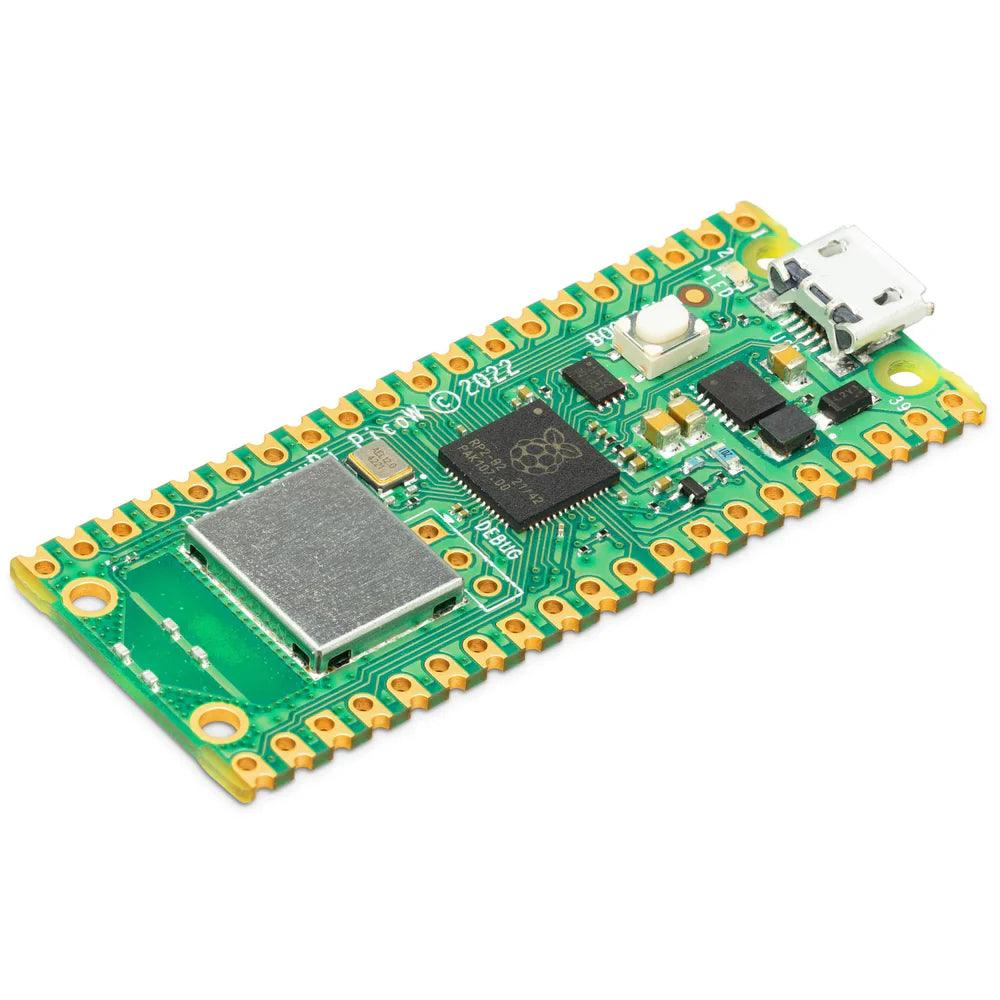
\includegraphics[width=0.9\linewidth, keepaspectratio]{images/components/pico_w.jpg} & 1 & 750.00 \\ \hline
\href{https://www.ram-e-shop.com/shop/ro-motor-tt-mini-dc-gearbox-motors-pair-2-motors-with-back-shaft-9455}{\textbf{\textcolor{darkblue}{DC Motors (TT Mini Gearbox Pair)}}} & 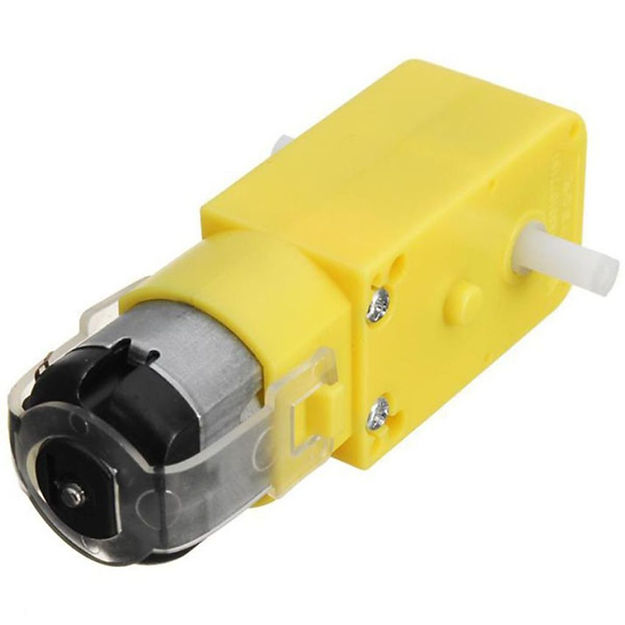
\includegraphics[width=0.9\linewidth, keepaspectratio]{images/components/dc_motor_tt.jpg} & 2 & 50.00 \\ \hline
\href{https://www.ram-e-shop.com/shop/kit-l298-red-l298-module-red-board-dual-h-bridge-motor-driver-using-l298n-7084}{\textbf{\textcolor{darkblue}{H-Bridge L298N Motor Driver}}} & 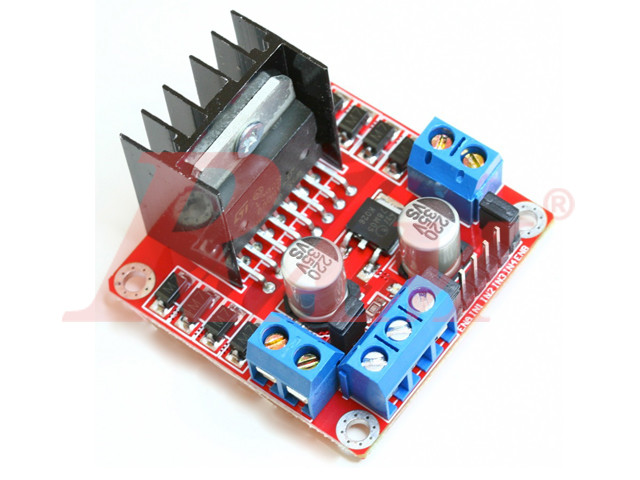
\includegraphics[width=0.9\linewidth, keepaspectratio]{images/components/l298n_driver.jpg} & 1 & 80.00 \\ \hline
\href{https://www.ram-e-shop.com/shop/kit-ultrasonic-hcsr04-ultrasonic-sensor-hc-sr04-5949}{\textbf{\textcolor{darkblue}{HC-SR04 Ultrasonic Sensor}}} & 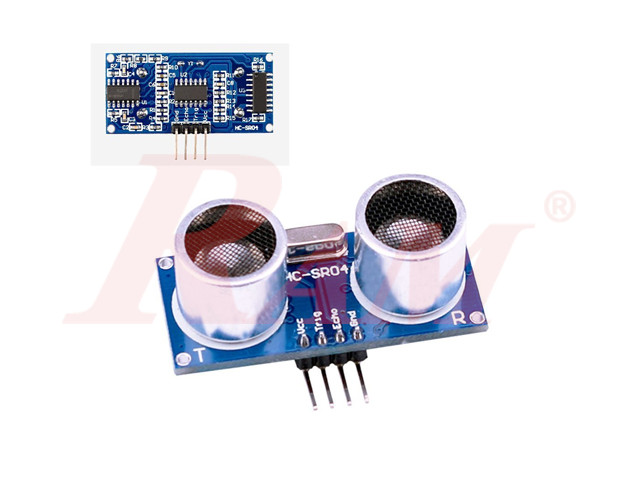
\includegraphics[width=0.9\linewidth, keepaspectratio]{images/components/hcsr04_sensor.jpg} & 1 & 40.00 \\ \hline
\href{https://www.ram-e-shop.com/shop/battery-li-12v-4000mah-battery-pack-12v-4000mah-6728}{\textbf{\textcolor{darkblue}{Battery Pack 12V 4000mAh}}} & 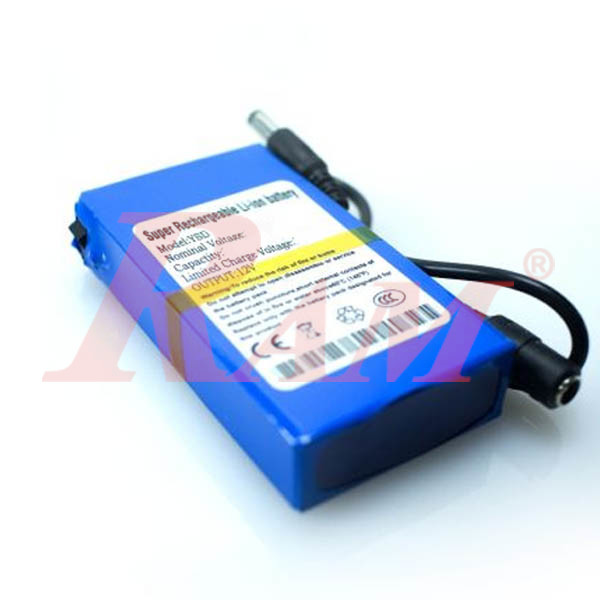
\includegraphics[width=0.9\linewidth, keepaspectratio]{images/components/battery_12v.jpg} & 1 & 1400.00 \\ \hline
\href{https://www.psdevwiki.com/ps3/Delta_KSB1012HE}{\textbf{\textcolor{darkblue}{PS3 Fan (Already Owned)}}} & 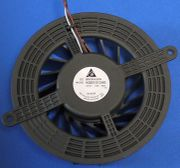
\includegraphics[width=0.9\linewidth, keepaspectratio]{images/components/ps3_fan.jpg} & 1 & 1000.00* \\ \hline
\href{https://www.ram-e-shop.com/shop/dc-dc-100-dc-dc-step-down-voltage-converter-adjustable-3a-lm2596s-4-38vdc-to-1-5-35vdc-sku-dc100-7257}{\textbf{\textcolor{darkblue}{DC-DC Step Down LM2596S}}} & 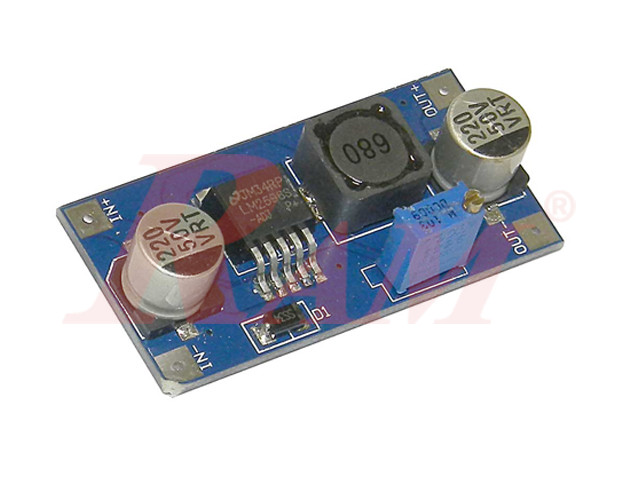
\includegraphics[width=0.9\linewidth, keepaspectratio]{images/components/lm2596s_buck.jpg} & 1 & 50.00 \\ \hline
\textbf{\textcolor{darkblue}{IR Photoelectric Encoder Sensor}} & 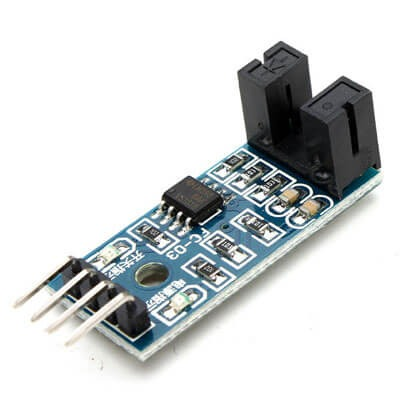
\includegraphics[width=0.9\linewidth, keepaspectratio]{images/components/encoder_sensor.jpg} & 2 & 25.00 \\ \hline
\textbf{\textcolor{darkblue}{Rotary Encoder Disc}} & 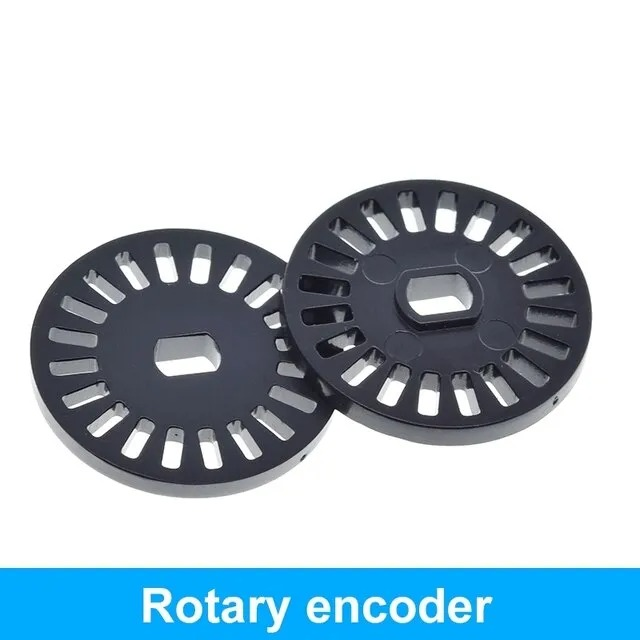
\includegraphics[width=0.9\linewidth, keepaspectratio]{images/components/encoder_disc.jpg} & 2 & 5.00 \\ \hline
\href{https://www.ram-e-shop.com/shop/pb-2-green-push-button-type-2-green-color-5614}{\textbf{\textcolor{darkblue}{Push Button (DS-316 Green)}}} & 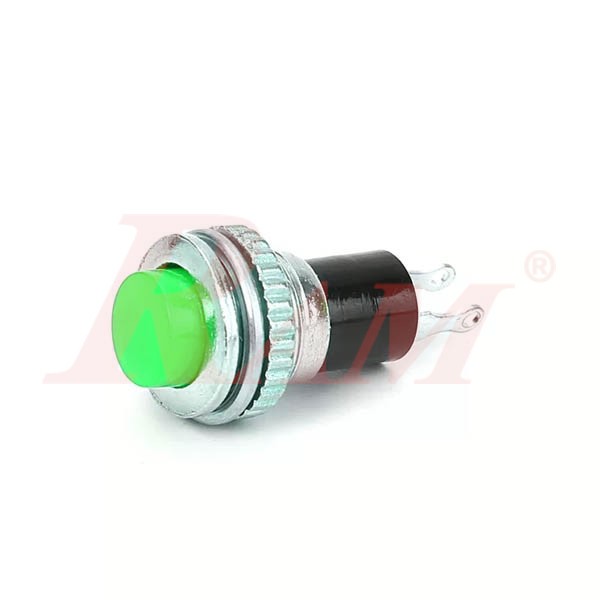
\includegraphics[width=0.9\linewidth, keepaspectratio]{images/components/push_button_green.jpg} & 1 & 7.50 \\ \hline
\href{https://www.ram-e-shop.com/shop/xd10-3-12vdc-green-xd10-3-dc12v-green-small-led-signal-indicator-light-10mm-9155}{\textbf{\textcolor{darkblue}{LED Indicator (XD10-3 Green)}}} & 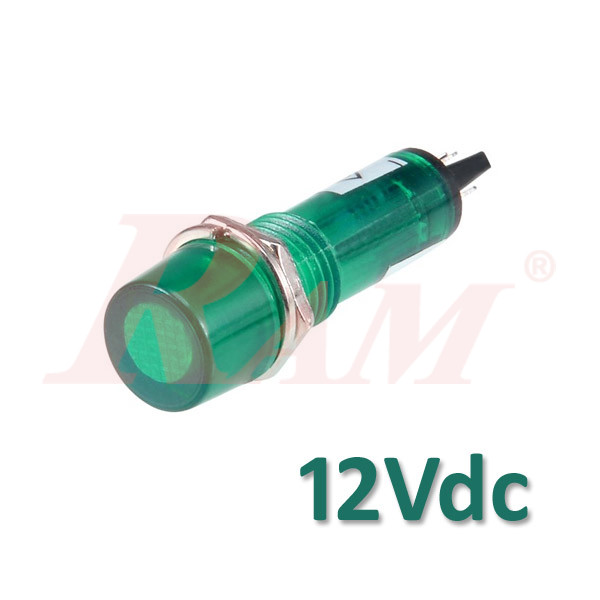
\includegraphics[width=0.9\linewidth, keepaspectratio]{images/components/led_indicator.jpg} & 1 & 7.00 \\ \hline
\href{https://www.ram-e-shop.com/shop/r-5-roseta-2pin-2-pin-pcb-screw-terminal-block-pitch-5mm-14-1mm-long-r-5-6323}{\textbf{\textcolor{darkblue}{2 Pin Screw Terminal}}} & 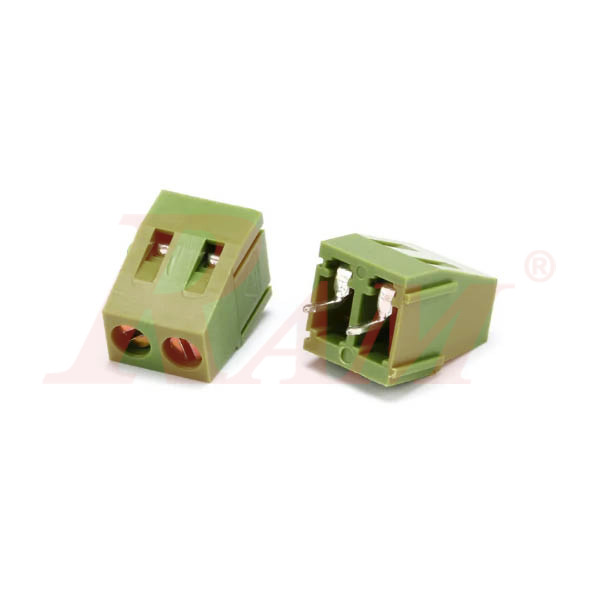
\includegraphics[width=0.9\linewidth, keepaspectratio]{images/components/terminal_2pin.jpg} & 3 & 5.00 \\ \hline
\href{https://www.ram-e-shop.com/shop/r-6-roseta-3pin-3-pin-pcb-screw-terminal-block-pitch-5mm-14-1mm-long-r-6-6322}{\textbf{\textcolor{darkblue}{3 Pin Screw Terminal}}} & 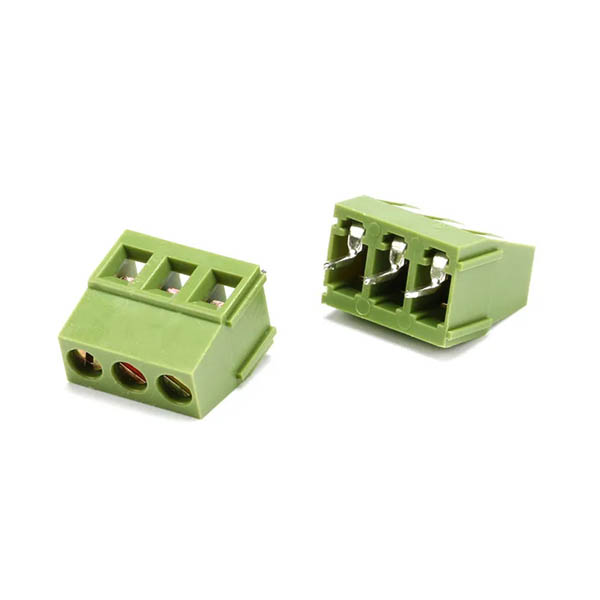
\includegraphics[width=0.9\linewidth, keepaspectratio]{images/components/terminal_3pin.jpg} & 6 & 6.00 \\ \hline
\href{https://www.ram-e-shop.com/shop/ph35-1x20-female-ph35-pin-header-female-1x20-straight-2-54mm-6529}{\textbf{\textcolor{darkblue}{Pin Header Female 1x20}}} & 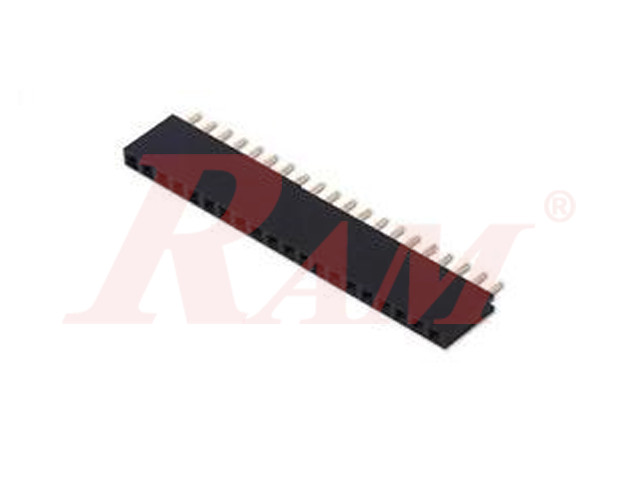
\includegraphics[width=0.9\linewidth, keepaspectratio]{images/components/pin_header_female.jpg} & 2 & 3.00 \\ \hline
{\textbf{\textcolor{darkblue}{Resistors (2.2k$\Omega$, 4.7k$\Omega$)}}} & 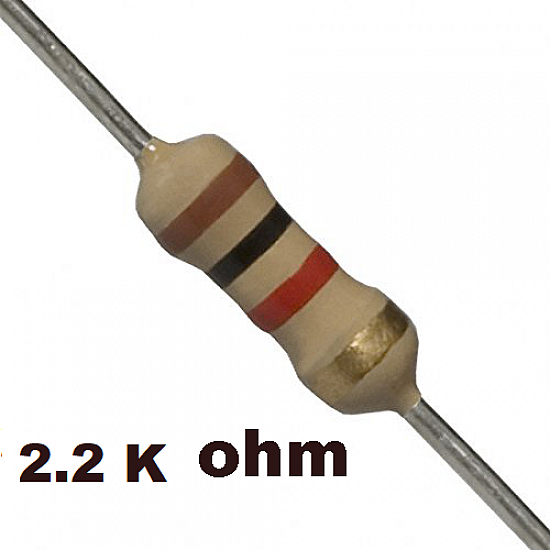
\includegraphics[width=0.9\linewidth, keepaspectratio]{images/components/resistor_2k2.png} & 2 & $\sim$2.00 \\ \hline
\href{https://www.ram-e-shop.com/shop/ph60-mf-20cm-ph60-20cm-male-to-female-40-jumper-wires-set-7066}{\textbf{\textcolor{darkblue}{Jumper Wires (Assorted)}}} & 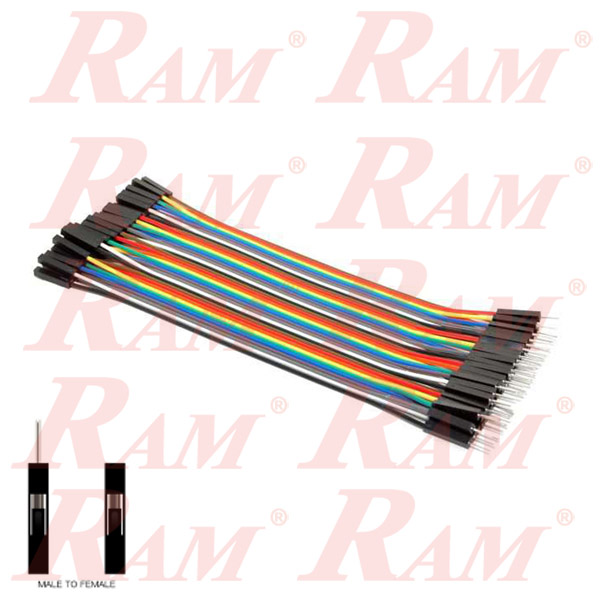
\includegraphics[width=0.9\linewidth, keepaspectratio]{images/components/jumper_mf.jpg} & 3 set & 35.00 \\ \hline
\href{https://www.ram-e-shop.com/shop/wire-speaker-2x1mm-speaker-wire-2-core-x-1mm-red-black-1-meter-8878}{\textbf{\textcolor{darkblue}{Speaker Wire (1m)}}} & 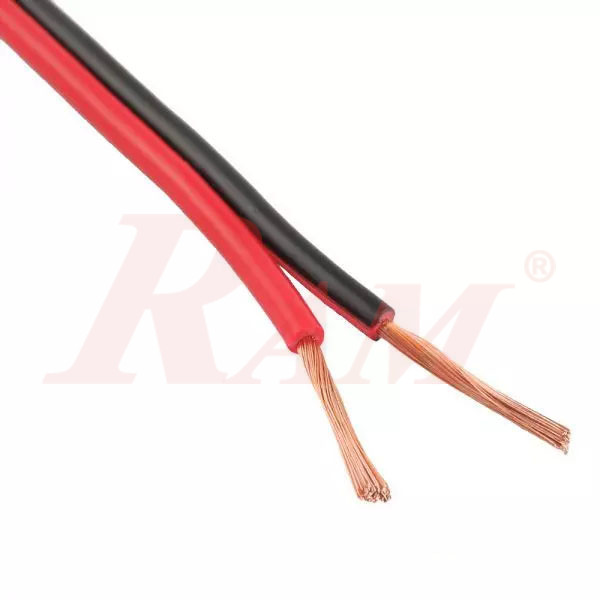
\includegraphics[width=0.9\linewidth, keepaspectratio]{images/components/speaker_wire.jpg} & 1 & 7.50 \\ \hline

% Mechanical Components
\href{https://www.maamoon.com/product-page/66mm-robot-smart-car-wheel-tyre}{\textbf{\textcolor{darkblue}{Robot Wheels (66mm)}}} & 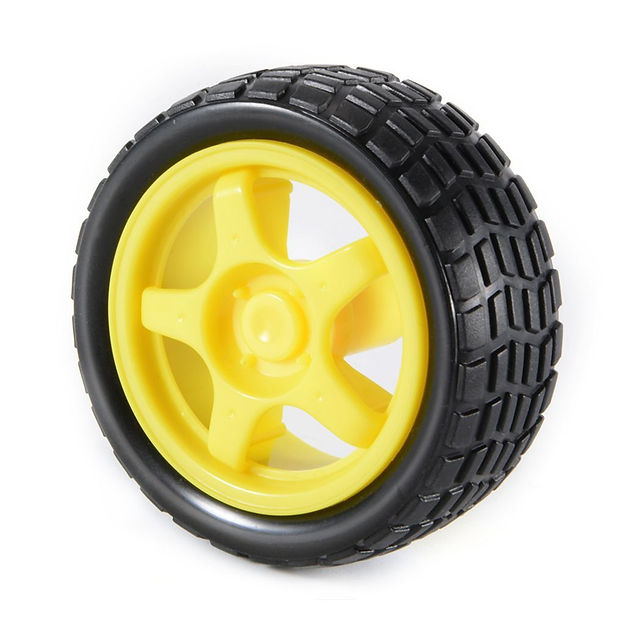
\includegraphics[width=0.9\linewidth, keepaspectratio]{images/components/wheel_66mm.jpg} & 2 & 36.00 \\ \hline
\href{https://www.ram-e-shop.com/shop/ro-wheel-caster-small-metal-caster-wheel-20-mm-robot-wheel-max-load-15kg-7010}{\textbf{\textcolor{darkblue}{Metal Caster Wheel}}} & 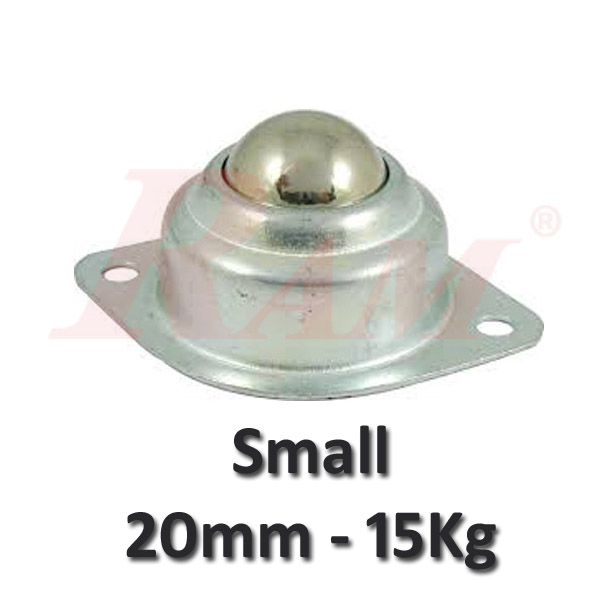
\includegraphics[width=0.9\linewidth, keepaspectratio]{images/components/caster_wheel.jpg} & 1 & 30.00 \\ \hline
\href{https://www.ram-e-shop.com/shop/spacer-screw-20mm-plastic-screw-shape-snap-in-rivet-pcb-spacer-20mm-5739}{\textbf{\textcolor{darkblue}{PCB Spacers (20mm)}}} & 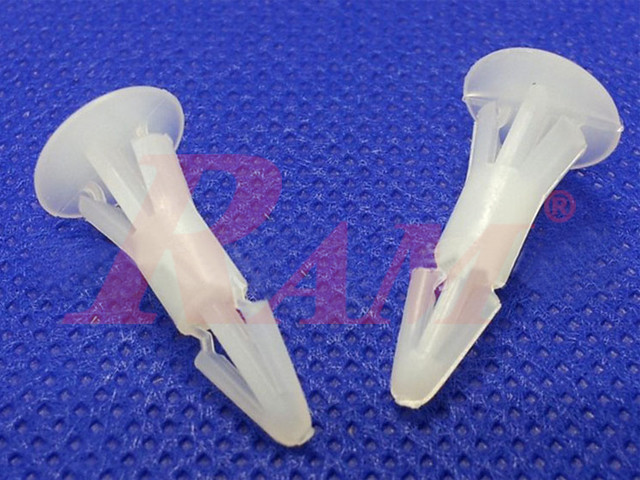
\includegraphics[width=0.9\linewidth, keepaspectratio]{images/components/pcb_spacer.jpg} & 8 & 0.75 \\ \hline
\href{https://www.ram-e-shop.com/shop/nail-3x05mm-bolt-m3x06-mm-100-screws-bag-6545}{\textbf{\textcolor{darkblue}{Bolts and Nuts (M3)}}} & 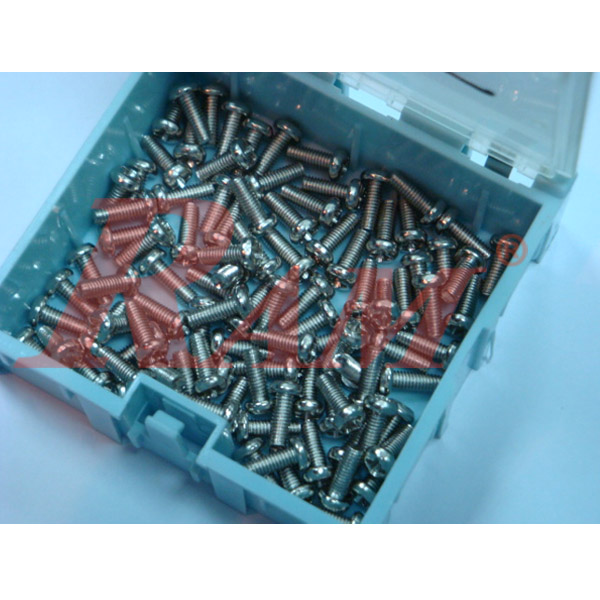
\includegraphics[width=0.9\linewidth, keepaspectratio]{images/components/bolts_m3.jpg} & 4 bag & 30.00 \\ \hline
\href{https://microohm-eg.com/product/6mm-electrical-waterproof-seal-heat-shrink-splice-wire-sleeve-yellow-1pcs/}{\textbf{\textcolor{darkblue}{Heat Shrink Sleeve}}} & 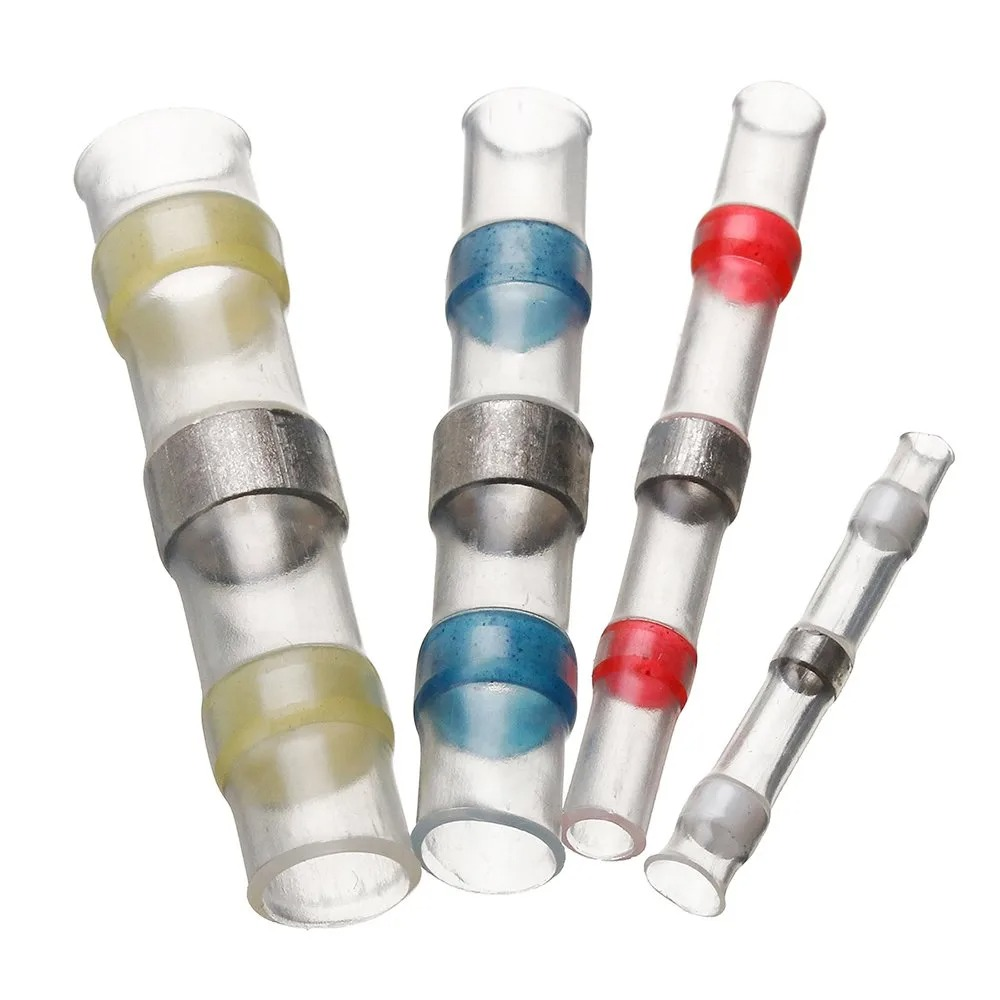
\includegraphics[width=0.9\linewidth, keepaspectratio]{images/components/heat_shrink.jpg} & 2 & 10.00 \\ \hline

\end{longtable}
\endgroup

\end{document}